\documentclass%
%[handout]%
{beamer}

\mode<presentation>
{
\useinnertheme{rounded}
\useoutertheme{infolines}
\usecolortheme{orchid}
\usecolortheme{whale}
}
%\setbeamertemplate{footline}{%
%  \raisebox{5pt}{\makebox[\paperwidth]{\hfill\makebox[10pt]{\scriptsize\insertframenumber}}}}

\usepackage[english]{babel}
\usepackage[latin1]{inputenc}
\usepackage{times}
\usepackage{../example-templates}
\usepackage{../pstricks-commands}
% psfrag needed for including latex labels on eps files created with xfig


\usepackage[T1]{fontenc}
% Or whatever. Note that the encoding and the font should match. If T1
% does not look nice, try deleting the line with the fontenc.

\graphicspath{{../../modules/}}

\newcommand{\currentLecture}{5}

\newcommand{\lect}[4]{
\ifnum#3=\currentLecture
  \date{#1}
  \lecture[#1]{#2}{#3}
#4
\else
%include nothing
\fi
}

\setbeamertemplate{footline}
{
  \leavevmode%
  \hbox{%
  \begin{beamercolorbox}[wd=.333333\paperwidth,ht=2.25ex,dp=1ex,center]{author in head/foot}%
    \usebeamerfont{author in head/foot}\insertshortauthor
  \end{beamercolorbox}%
  \begin{beamercolorbox}[wd=.333333\paperwidth,ht=2.25ex,dp=1ex,center]{title in head/foot}%
    \usebeamerfont{title in head/foot}\insertshorttitle
  \end{beamercolorbox}%
  \begin{beamercolorbox}[wd=.333333\paperwidth,ht=2.25ex,dp=1ex,center]{date in head/foot}%
    \usebeamerfont{date in head/foot}\insertshortdate{}
  \end{beamercolorbox}}%
  \vskip0pt%
}

\setbeamertemplate{navigation symbols}{}


\renewcommand{\Arcsin}{\arcsin}
\renewcommand{\Arccos}{\arccos}
\renewcommand{\Arctan}{\arctan}
\renewcommand{\Arccot}{\text{arccot\hspace{0.03cm}}}
\renewcommand{\Arcsec}{\text{arcsec\hspace{0.03cm}}}
\renewcommand{\Arccsc}{\text{arccsc\hspace{0.03cm}}}


% If you have a file called "university-logo-filename.xxx", where xxx
% is a graphic format that can be processed by latex or pdflatex,
% resp., then you can add a logo as follows:

%\pgfdeclareimage[height=0.8cm]{logo}{bluelogo}
%\logo{\pgfuseimage{logo}}

\begin{document}

\AtBeginLecture{%

\title[\insertlecture]{Math 141}
\subtitle{\insertlecture}
\author[Math 141]{Catalin Zara  \\~\\\small{with modifications by  Todor Milev}\normalsize}
\institute[UMass Boston]{University of Massachusetts Boston}
\date{\insertshortlecture}
\begin{frame}
  \titlepage
\end{frame}

\begin{frame}{Outline}
  \tableofcontents[pausesections]
\end{frame}
}%

% begin lecture
\lect{2014}{Lecture  1}{1}{

\input{../../modules/course-outline/course-outline-multivariable-calculus-UMB-242-Catalin-Zara}
}

% begin lecture
\lect{2014}{Lecture  2}{2}{
\section{Space}

\begin{frame}
\frametitle{Space}
\begin{itemize}
\item<1-> Some subsets of points in space are special/distinguished.
\begin{itemize}
\item<2-> Lines.
\item<3-> Planes.
\end{itemize}
\item<4-> We rely on intuition rather than axiomatic construction.
\item<5-> Given a pair of objects (lines or planes), we discuss all possible configurations with respect to: 
\begin{itemize}
\item<6-> inclusion
\item<7-> intersection
\item<8-> parallelism
\item<9-> being contained in a single plane (being ``co-planar'').
\end{itemize}
\end{itemize}
\end{frame}

\begin{frame}
\frametitle{Configurations of pair of lines}
\small
\begin{tabular}{c|r|cccc}
& pair of objects &  intersection& parallelism & co-planar?\\\hline
\multirow{3}{*}{\rotatebox{90}{\mbox{2 lines}}}
& intersecting lines&  one point & not parallel& yes\\
& parallel lines&  empty & parallel & yes \\
& skew lines &  none & not parallel & no\\
\hline 
\multirow{3}{*}{\rotatebox{90}{
\begin{tabular}{r}
line \&  \\ plane
\end{tabular}
}}
& line intersecting plane &  one point & not parallel & no\\
& line parallel to a plane & none & parallel & no\\
& line lying in plane & line & - & yes\\
\hline 
\multirow{2}{*}{\rotatebox{90}{\mbox{2 planes}}}
& intersecting planes & line & not parallel & -\\
& parallel planes & none & parallel & -\\
\end{tabular}

\normalsize
\medskip
\psset{xunit=1cm, yunit=1cm}
\begin{pspicture}(-3, -3)(3,3)
\fcPolyLineIIId{[-1 -1 0] [1 -1 0] [1 1 0] [-1 1 0] [-1 -1 0]}
\end{pspicture}
\end{frame}

\begin{frame}
\frametitle{Example}

%
\begin{figure}[h]
  \psfrag{A}{$A$} 
  \psfrag{B}{$B$} 
  \psfrag{C}{$C$} 
  \psfrag{D}{$D$}  
  \psfrag{E}{$E$} 
  \psfrag{F}{$F$}  
  \psfrag{G}{$G$}   
  \psfrag{L1}{$L_1$} 
  \psfrag{L2}{$L_2$} 
  \psfrag{L3}{$L_3$}  
  \psfrag{L4}{$L_4$} 
  \psfrag{cP}{$\cP$}     
  \includegraphics[height=2in]{./images/line_plane.eps}
  \caption{Points, lines, and planes}
  \label{fig:points_lines_planes}
\end{figure}
%
\end{frame}
\begin{frame}
 \frametitle{Distance}

\begin{itemize}
 \item Euclidean Plane: \\
    Through a point $P$ outside a line $L$\\ there passes at most one line $\ell$ parallel to $L$
  \item<2-> Distance - Primordial concept \\
      Quantifies/Measures how close/far apart are any two points \\
      $$d(A,B) = |AB|$$
  \item<3-> Measures of angles $\to$ Perpendicularity
      \begin{itemize}
	\item Line and Line
        \item Line and Plane
        \item Plane and Plane
      \end{itemize}
  \end{itemize}

\end{frame}
\input{../../modules/coordinate-systems/orthogonality}
\begin{frame}
 \frametitle{Rectangular/Cartesian Coordinates}

 \begin{itemize}
  \item To reach the projector: \pause Must relate its position to
      \begin{itemize}
	\item My current position
	\item My current orientation
      \end{itemize}

  \item<3-> Rectangular Coordinate System
      \begin{itemize}
	\item Position $\to$ Origin $\to$ $O$;
	\item Orientation $\to$ Fundamental directions $\to$ Ahead-Left-Up;
	\item Displacement $\to$ measured using the distance:
	    \begin{itemize}
	      \item Positive in Ahead, Left, and Up directions;
	      \item Negative in Back, Right, and Down directions.
	    \end{itemize}
	\end{itemize}

  \item<4-> Example: Projector $P \to (x,y,z) = (3,1,2)$ or $P(3,1,2)$.

  \item<5-> Using a fixed coordinate system:
    \begin{itemize}
      \item $\text{Space } \simeq \RR \times \RR \times \RR = \RR^3$
      \item $\text{Plane } \simeq \RR \times \RR = \RR^2$
    \end{itemize}
 \end{itemize}
\end{frame}

\begin{frame}
%
\begin{table}[h]
\begin{tabular}{lcr}
  \psfrag{P}{Projector}
  \psfrag{O}{Me}  
  \psfrag{x}{$x$} 
  \psfrag{y}{$y$} 
  \psfrag{z}{$z$}     
  \psfrag{A}{Ahead}
  \psfrag{L}{Left}
  \psfrag{U}{Up}  
  \includegraphics[height=2in]{./images/projector.eps}
%
& \hspace{2cm} &
%
%\begin{figure}[h]
  \psfrag{P}{$P(a,b,c)$}
  \psfrag{O}{$O(0,0,0)$}  
  \psfrag{x}{$a$} 
  \psfrag{y}{$b$} 
  \psfrag{z}{$c$}     
  \psfrag{A}{$Ox$}
  \psfrag{L}{$Oy$}
  \psfrag{U}{$Oz$}  
  \includegraphics[height=2in]{../../modules/coordinate-systems/pictures/projector.eps}
%
\end{tabular}
  \end{table}
%
\end{frame}
\begin{frame}[label=current]
\frametitle{Euclidean Distance in Coordinates}
\begin{definition}
The distance between the points $A(x_A,y_A,z_A)$ and $B(x_B,y_B,z_B)$ is given by:
\[
d(A,B) = |AB| = \sqrt{(x_B-x_A)^2+(y_B-y_A)^2+(z_B-z_A)^2}
\]
\end{definition}
\begin{columns}
\column{0.4\textwidth}
\psset{xunit=1cm, yunit=1cm}
\begin{pspicture}(-2, -2)(2,2)
\renewcommand{\fcScreen}{[-0.5 1 -0.2] -1}
\tiny
\fcAxesIIId{3}{3}{3}
\fcPolyLineIIId[linecolor=red]{[2.6 1 1][2.6 1.4 1] [3 1.4 1] }
\fcPolyLineIIId[linecolor=red]{[2.8 3.7 1][2.8 3.7 1.360555128] [3 4 1.360555128] }

\fcPolyLineIIId[linestyle=dotted]{ [1 1 1] [1 4 1] [1 4 3]}
\fcLineIIId[linestyle=dotted]{[1 4 1]}{[3 4 1]}
\fcParallelogramHollowIIId{ [1 1 1] }{ [3 1 1] }{ [3 1 3] }
\fcParallelogramHollowIIId{ [1 1 3] }{ [3 1 3] }{ [3 4 3] }
\fcParallelogramHollowIIId{ [3 1 1] }{ [3 4 1] }{ [3 4 3] }
\fcLineIIId[linestyle=dotted]{[1 1 1]}{[3 4 1]}
\fcLineIIId[linestyle=dotted]{[1 1 1]}{[3 4 3]}
\fcPutIIId[t]{[1 1 0.9]}{$A$}
\fcPutIIId[l]{[3 4 3]}{$~~B$}
\fcPutIIId[l]{[3 4 1]}{$~~C$}
\fcPutIIId[t]{[3 1 0.9]}{$D$}

\fcPutIIId[t]{[2 1 0.9]}{$x_B- x_A$}
\fcPutIIId[tl]{[3 2.5 1]}{$~~y_B- y_A$}

\fcPutIIId[l]{[3 4 2]}{$~~z_B- z_A$}
\end{pspicture}
\column{0.6\textwidth}
Motivation. 

Pythagorean theorem for $\triangle ADC$: $|AC|^2 = |AD|^2+|DC|^2$.
Pythagorean theorem for $\triangle ACB$: $|AB|^2 =|AC|^2+ |BC|^2= |AD|^2+|DC|^2+|BC|^2 = (x_B-x_A)^2+(y_B-y_A)^2+(z_B-z_A)^2$.
\end{columns}

%\psfrag{O}{$O$}
%\psfrag{A}{$A$} 
%\psfrag{B}{$B(x_B, y_B, z_B)$}  
%\psfrag{C}{$C(x_B, y_B, z_A)$}    
%\psfrag{x}{$y$} 
%\psfrag{y}{$x$} 
%\psfrag{z}{$z$}     
%\psfrag{dx}{$y_B - y_A$}
%\psfrag{dy}{$x_B - x_A$}
%\psfrag{dz}{$z_B - z_A$}  
%\includegraphics[height=1in]{../../modules/coordinate-systems/pictures/euclidean_distance.eps}
%
%
Example: $P(3,1,2)$ and $Q(1,2,3)$:\pause
%
$$D(P,Q) = \sqrt{(1-3)^2+(2-1)^2+(3-2)^2} = \sqrt{6}\; .$$

\end{frame}
\begin{frame}
 \frametitle{Change of Coordinates}

  Change in original position and orientation $\to$ new coordinates

\pause

Example:
  \begin{itemize}
   \item Move ahead 1m;
   \item Turn a quarter of a circle to the right.
  \end{itemize}
  
%
\begin{table}[h]
\begin{tabular}{lcr}
  \psfrag{P}{$P(3,1,2)$}
  \psfrag{O}{$O(0,0,0)$}  
  \psfrag{x}{$x=3$} 
  \psfrag{y}{$y=1$} 
  \psfrag{z}{$z=2$}     
  \psfrag{A}{$Ox$}
  \psfrag{L}{$Oy$}
  \psfrag{U}{$Oz$}  
  \includegraphics[height=2in]{./images/projector.eps}
%
& \hspace{2cm} &
%
\psfrag{P}{$P$}
  \psfrag{Op}{$O'$} 
  \psfrag{O}{$O$}  
  \psfrag{L}{$L$}
  \psfrag{U}{$U$}   
  \psfrag{xp}{$x'=-1$} 
  \psfrag{yp}{$y'=2$} 
  \psfrag{zp}{$z'=2$}     
  \psfrag{Ap}{$A'$}
  \psfrag{Lp}{$L'$}
  \psfrag{Up}{$U'$}  
  \includegraphics[height=2in]{./images/new_frame.eps}
%
\end{tabular}
  \end{table}
%  
%
\pause  
New coordinates of projector: $P \to (x',y',z') = (-1,2,2)$
\end{frame}

\begin{frame}
\frametitle{General formula for this change of coordinates}
%
\begin{table}[h]
\begin{tabular}{lcr}
  \psfrag{P}{$P(x,y,z)$}
  \psfrag{O}{$O(0,0,0)$}  
  \psfrag{x}{$x$} 
  \psfrag{y}{$y$} 
  \psfrag{z}{$z$}     
  \psfrag{A}{$Ox$}
  \psfrag{L}{$Oy$}
  \psfrag{U}{$Oz$}  
  \includegraphics[height=2in]{./images/projector.eps}
%
& \hspace{2cm} &
%
\psfrag{P}{$P(x', y', z')$}
  \psfrag{Op}{$O'$} 
  \psfrag{O}{$O$}  
  \psfrag{L}{$L$}
  \psfrag{U}{$U$}   
  \psfrag{xp}{$x'=-y$} 
  \psfrag{yp}{$y'=x-1$} 
  \psfrag{zp}{$z'=z$}     
  \psfrag{Ap}{$A'$}
  \psfrag{Lp}{$L'$}
  \psfrag{Up}{$U'$}  
  \includegraphics[height=2in]{./images/new_frame.eps}
%
\end{tabular}
  \end{table}
%  

\begin{eqnarray*}
 x' = & -y \\
 y' = & x-1 \\
 z' = & z
\end{eqnarray*}
%
Example $Q(x=1,y=2,z=3) \leftrightarrow Q(x'=-2, y'=0,z'=3)$

\end{frame}



\begin{frame}
 \frametitle{Fundamental Philosophy}
  $P(3,1,2)$ and $Q(1,2,3)$ in $(x,y,z)-$coordinates

  $P(-1,2,2)$ and $Q(-2,0,3)$ in $(x',y'z')-$coordinates

  Distance in new coordinates:
 \pause
%
$$d_{x',y',z'}(P,Q) = \sqrt{(-2+1)^2+(0-2)^2+(3-2)^2} = \sqrt{6} = d_{x,y,z}(P,Q)$$

Fundamental Philosophy:\pause
\begin{itemize}
 \item Space doesn't come with coordinates
  \item Natural concepts (such of distance) are independent of coordinates
  \item If a natural concept is defined using coordinates, \\
          the result does not depend on the chosen coordinate system.
\end{itemize}


\end{frame}
\begin{frame}
  \frametitle{Sets in Space}

  $X$ subset of a set $Y$:

  $$X = \{ A \text{ in } Y | A \text{ has property } \mathcal{P} \} \subset Y$$

\pause
Examples  (Fixed point $Q$, fixed $r>0$):

$$X = \{ A \text{ in Space } | d(A,Q) = r \} = S_r(Q)\; ,$$
\pause Sphere of radius $r$ centered at $Q$.\pause

$$B_r(Q) = \{ A \text{ in Space } | d(A,Q) <r \} \; ,$$
\pause  Open ball of radius $r$ centered at $Q$. \pause

$$\overline{B}_r(Q) = \{ A \text{ in Space } | d(A,Q) \leqslant r\} \; ,$$
\pause  Closed ball of radius $r$ centered at $Q$.

\end{frame}
\begin{frame}
 \frametitle{Equation(s) of Subsets}

  $$X = \{ (x,y,z) | x,y,z \text{ satisfy certain relation(s) } \} \; .$$

\pause
Examples:

$\{(x,y,z) | x^2+y^2+z^2 = 1\}$:

\pause
sphere of radius $r=1$ centered at the origin $(0,0,0)$

Also refered to as: sphere $x^2+y^2+z^2 = 1$

\pause
\medskip

$\{ (x,y,z) | x=0 \}$: coordinate Left-Up plane

\pause
\medskip

$\{ (x,y,z) | x=0 \text{ and } y=0 \}$:

intersection of coordinate planes $\rightarrow$ coordinate axis

\pause
\medskip

Can be given by only one equation:

$x^2+y^2 = 0$ $\rightarrow$ $x=0$,$y=0$, and $z$ arbitrary $\rightarrow$

vertical axis above $(0,0)$ in $(x,y)-$plane

\pause
\medskip

Important: Equations in Plane vs. Space.

\end{frame}
\begin{frame}
 \frametitle{Recognizing Spheres from Equations}

  $Q(x_0,y_0,z_0)$, $r>0$, $A(x,y,z)$. Remark: $d(A,Q) = r \longleftrightarrow d^2(A,Q) = r^2$

$$S_r(Q): \quad (x-x_0)^2+(y-y_0)^2+(z-z_0)^2 = r^2$$

\pause
Example:
$$(x-2)^2+(y-0)^2+(z+1)^2=3^2$$
%
$$x^2+y^2+z^2 -4x + 2z -4=0$$

\pause
\begin{itemize}
 \item no mixed terms $xy$, $xz$, or $yz$;
 \item quadratic terms $x^2$, $y^2$, and $z^2$ with the same coefficient.
\end{itemize}

\pause
Examples:
$$x^2+y^2+z^2-4x+2y=0$$
%
\pause
Complete the square:
%
$$(x-2)^2 + (y+1)^2 +z^2 = 5$$
%
Sphere of radius $\sqrt{5}$ centered at $(2,-1,0)$.

\pause
How about $x^2+y^2+z^2 - 4x+2y = -6$? \pause Passes both tests, but ...
%
$$(x-2)^2 + (y+1)^2 +z^2 = -1$$
%
is impossible! No such points, set is empty.

\end{frame}

\section{Polar Coordinates}
% begin module polar-intro
\begin{frame}[t]
\frametitle{Polar Coordinates}
\begin{itemize}
\item<1->  The polar coordinates system is an alternative to the Cartesian coordinates system.
%\item  Instead of specifying horizontal distance and vertical distance, we specify angle and distance from the origin.
\item<2->  Choose a point in the plane called $O$ (the origin).
\item<3->  Draw a ray starting at $O$. The ray is called the polar axis.  This ray is usually drawn horizontally to the right.
\end{itemize}
\begin{columns}[c]
\column{.5\textwidth}
\psset{xunit=5cm, yunit=5cm}
\begin{pspicture}(-0.2, -0.2)(1.500000,0.6)
\tiny
%force a boudning box:
\psline[linecolor=red!1](-0.1, -0.1)(-0.21,0.2)
\psline[linecolor=red!1](1.1, 0.6)(1.1,0.61)

\uncover<5->{
%Calculator input: plotCurve{}(1/5 \cos{}t, 1/5 \sin{}t, 0, 1/6 \pi)
\parametricplot[arrows=->, linecolor=red, plotpoints=1000] {0}{0.523599}{t 57.29578 mul cos 0.2 mul t 57.29578 mul sin 0.2 mul }
\psline[linecolor=blue](0,0)(0.866025404, 0.5)
\rput(0.22, 0.06){$\alert<5>{\theta}$}
}

\uncover<4->{
\fcFullDotBlue{0.866025404}{0.5}
\rput[l](0.88, 0.5){$P\uncover<7->{\alert<7>{(r,\theta)}}$}
}

\uncover<2->{
\fcFullDotBlue{0}{0}
\rput(-0.1, 0){$O$}
}
\uncover<6->{
\rput(0.4, 0.3){$\alert<6>{r}$}
}
\uncover<3->{
\psline{->}(0,0)(1,0)
\rput (0.5, -0.05){polar axis}
}
\end{pspicture}

\vspace{1cm}

%\includegraphics[height=4cm]{polar-curves/pictures/11-03-polar.pdf}%
\column{.5\textwidth}
\begin{itemize}
\only<1-7>{\item<4->  Let $P$ be a point in the plane.
\item<5->  Let $\theta$ denote the angle between the polar axis and the line $OP$.
\item<6->  Let $r$ denote the length of the segment $OP$.
\item<7->  Then $P$ is represented by the ordered pair $(r, \theta )$.
}
\only<8->{
\item<8->  The letters $(x,y)$ imply Cartesian coordinates and the letters $(\rho, \theta)$- polar. \uncover<9->{When we use other letters, it should be clear from context whether we mean Cartesian or polar coordinates.} \uncover<10->{If not, one must request clarification.}
}
\end{itemize}
\end{columns}
\end{frame}
% end module polar-intro

% begin module polar-questions
\begin{frame}
\begin{enumerate}
\item<1-| alert@2>  What if $\theta$ is negative?
\item<1-| alert@3>  What if $r$ is negative?
\item<1-| alert@4>  What if $r$ is $0$?
\end{enumerate}
\begin{columns}[c]
\column{.5\textwidth}
\uncover<2->{
\psset{xunit=2cm, yunit=2cm}
\begin{pspicture}(-0.9, -1.2)(2,0.2)
\tiny
%force a boudning box:
%\psline[linecolor=red!1](-0.1, -0.1)(-0.21,0.2)
%\psline[linecolor=red!1](1.1, 0.6)(1.1,0.61)
\fcFullDotBlue{0}{0}

%Calculator input: plotCurve{}(1/10 \cos{}t, 1/10 \sin{}t, 0, -3/4 \pi)
\parametricplot[arrows=->, linecolor=\fcColorGraph, plotpoints=100]{0} {-2.35619} {t 57.29578 mul cos 0.3000000 mul t 57.29578 mul sin 0.3000000 mul }
\rput[t] (0,-0.1){$O$}
\rput[l](0.3, -0.2){$\theta=-\frac{3\pi}{4}$}

\psline{->}(0,0)(2,0)
\psline[linecolor=blue](0,0)(-0.707106781, -0.707106781)
\fcFullDotBlue{-0.707106781}{-0.707106781}
\rput[tl](-0.6, -0.7){$\begin{array}{l}(\rho,\theta)=\left(1, -\frac{3\pi}{4}\right)\\ (x,y)=\left(-\frac{\sqrt{2}}2, -\frac{\sqrt{2}}2 \right) \end{array}$}
\end{pspicture}
}

\uncover<3->{
\psset{xunit=2cm, yunit=2cm}
\begin{pspicture}(-0.9, -1.5)(1.7,0.8)
\tiny
%force a boudning box:
%\psline[linecolor=red!1](-0.1, -0.1)(-0.21,0.2)
%\psline[linecolor=red!1](1.1, 0.6)(1.1,0.61)
\fcFullDotBlue{0}{0}

\parametricplot[arrows=->, linecolor=\fcColorGraph, plotpoints=100]{0} {0.523598776 } {t 57.29578 mul cos 0.3000000 mul t 57.29578 mul sin 0.3000000 mul }
\parametricplot[arrows=->, linecolor=brown, plotpoints=100]{0} {3.665191429 } {t 57.29578 mul cos 0.25 mul t 57.29578 mul sin 0.25 mul }

\rput[t] (0,-0.1){$O$}

\psline{->}(0,0)(1,0)
\psline[linecolor=blue](0,0)(0.866025404, 0.5)
\fcFullDotBlue{0.866025404}{0.5}
\rput[tl](-0.75, -0.5){
$(-\rho, \theta)$
}
\fcFullDotBlue{-0.866025404}{-0.5}
\psline[linecolor=blue, linestyle=dashed](0,0) (-0.866025404,-0.5)
\rput[tl](0.6, 0.7){$(\rho, \theta) $}
\end{pspicture}
}
%\ \uncover<2->{%
%\includegraphics[height=3cm]{polar-curves/pictures/11-03-ex1b.pdf}%
%}%
%\ \uncover<3->{%
%\includegraphics[height=3cm]{polar-curves/pictures/11-03-negativer.pdf}%
%}%
\column{.5\textwidth}
\begin{enumerate}
\item<2-| alert@2>  Positive angles $\theta$ are measured in the counterclockwise direction from $O$.  Negative angles are measured in the clockwise direction.
\item<3-| alert@3>  Points with polar coordinates $(-r, \theta)$ and $(r, \theta)$ lie on the same line through $O$ and at the same distance from $O$, but on opposite sides.
\item<4-| alert@4>  If $r = 0$, then $(r, \theta) = P = O$ for all values of $\theta$.
\end{enumerate}
\end{columns}
\end{frame}
% end module polar-questions

% begin module polar-many-representations
\begin{frame}
\begin{columns}[c]
\column{.5\textwidth}
\uncover<1->{
\psset{xunit=2cm, yunit=2cm}
\begin{pspicture}(-0.9, -1.1)(2,0.5)
\tiny
%force a boudning box:
%\psline[linecolor=red!1](-0.1, -0.1)(-0.21,0.2)
%\psline[linecolor=red!1](1.1, 0.6)(1.1,0.61)
\fcFullDotBlue{0}{0}

%Calculator input: plotCurve{}(1/10 \cos{}t, 1/10 \sin{}t, 0, -3/4 \pi)
\parametricplot[arrows=->, linecolor=\fcColorGraph, plotpoints=100]{0} {3.926990817} {t 57.29578 mul cos 0.3000000 mul t 57.29578 mul sin 0.3000000 mul }
\rput[t] (0,-0.1){$O$}
\rput[l](0.3, 0.3){$\theta=\frac{5\pi}{4}$}

\psline{->}(0,0)(2,0)
\psline[linecolor=blue](0,0)(-0.707106781, -0.707106781)
\fcFullDotBlue{-0.707106781}{-0.707106781}
\rput[tl](-0.6, -0.7){$(r,\theta)=\left(1, \frac{5\pi}{4}\right)$}
\end{pspicture}
}
\uncover<2->{
\psset{xunit=2cm, yunit=2cm}
\begin{pspicture}(-0.9, -1.1)(2,0.5)
\tiny
%force a boudning box:
%\psline[linecolor=red!1](-0.1, -0.1)(-0.21,0.2)
\psline[linecolor=red!1](1.1, 0.5)(1.1,0.51)
\fcFullDotBlue{0}{0}

%Calculator input: plotCurve{}(1/10 \cos{}t, 1/10 \sin{}t, 0, -3/4 \pi)
\parametricplot[arrows=->, linecolor=\fcColorGraph, plotpoints=100]{0} {-2.35619} {t 57.29578 mul cos 0.3000000 mul t 57.29578 mul sin 0.3000000 mul }
\rput[t] (0,-0.1){$O$}
\rput[l](0.3, -0.2){$\theta=-\frac{3\pi}{4}$}

\psline{->}(0,0)(2,0)
\psline[linecolor=blue](0,0)(-0.707106781, -0.707106781)
\fcFullDotBlue{-0.707106781}{-0.707106781}
\rput[tl](-0.6, -0.7){$(r,\theta)=\left(1, -\frac{3\pi}{4}\right)$}
\end{pspicture}
}

%\ \uncover<1->{%
%\includegraphics[height=3cm]{polar-curves/pictures/11-03-ex1a.pdf}%
%}%

%\ \uncover<2->{%
%\includegraphics[height=3cm]{polar-curves/pictures/11-03-ex1b.pdf}%
%}%
\column{.5\textwidth}
\uncover<3->{
\psset{xunit=2cm, yunit=2cm}
\begin{pspicture}(-0.9, -1.1)(2,0.5)
\tiny
%force a boudning box:
%\psline[linecolor=red!1](-0.1, -0.1)(-0.21,0.2)
%\psline[linecolor=red!1](1.1, 0.6)(1.1,0.61)
\fcFullDotBlue{0}{0}

%Calculator input: plotCurve{}(1/50 t \cos{}t+3/20 \cos{}t, 1/50 t \sin{}t+3/20 \sin{}t, 0, 13/4 \pi)
\parametricplot[arrows=->, linecolor=\fcColorGraph, plotpoints=400] {0} {10.2102} {t 57.29578 mul cos 0.1500000 mul t 57.29578 mul cos t mul 0.0200000 mul add t 57.29578 mul sin 0.1500000 mul t 57.29578 mul sin t mul 0.0200000 mul add }

\rput[t] (0,-0.1){$O$}
\rput[l](0.3, 0.3){$\theta=\frac{13\pi}{4}$}

\psline{->}(0,0)(2,0)
\psline[linecolor=blue](0,0)(-0.707106781, -0.707106781)
\fcFullDotBlue{-0.707106781}{-0.707106781}
\rput[tl](-0.6, -0.7){$(r,\theta)=\left(1, \frac{13\pi}{4}\right)$}
\end{pspicture}
}

\uncover<4->{
\psset{xunit=2cm, yunit=2cm}
\begin{pspicture}(-0.9, -1.1)(2,0.5)
\tiny
%force a boudning box:
%\psline[linecolor=red!1](-0.1, -0.1)(-0.21,0.2)
\psline[linecolor=red!1](1.1, 0.5)(1.1,0.51)
\fcFullDotBlue{0}{0}

%Calculator input: plotCurve{}(1/10 \cos{}t, 1/10 \sin{}t, 0, -3/4 \pi)
\parametricplot[arrows=->, linecolor=\fcColorGraph, plotpoints=100]{0} {0.785398163} {t 57.29578 mul cos 0.3000000 mul t 57.29578 mul sin 0.3000000 mul }
\rput[t] (0,-0.1){$O$}
\rput[l](0.35, 0.15){$\theta=\frac{\pi}{4}$}

\psline{->}(0,0)(2,0)
\psline[linecolor=blue](0,0)(-0.707106781, -0.707106781)
\fcFullDotBlue{-0.707106781}{-0.707106781}
\psline[linestyle=dashed](0,0)(0.707106781, 0.707106781)
\fcFullDotBlack{0.707106781}{0.707106781}
\rput[tl](-0.6, -0.7){$(r,\theta)=\left(-1, \frac{\pi}{4}\right)$}
\end{pspicture}
}
%\ \uncover<3->{%
%\includegraphics[height=3cm]{polar-curves/pictures/11-03-ex1c.pdf}%
%}%

%\ \uncover<4->{%
%\includegraphics[height=3cm]{polar-curves/pictures/11-03-ex1d.pdf}%
%}%
\end{columns}
\begin{itemize}
\item  There are many ways to represent the same point.
\item<2-| alert@2>  We could use a negative $\theta$.
\item<3-| alert@3>  We could go around more than once.
\item<4-| alert@4>  We could use a negative $r$.
\end{itemize}
\end{frame}
% end module polar-many-representations

%begin module polar-two-points-coincide-iff
\begin{frame}
\begin{itemize}
\item Let $P_1$ be point  with polar coordinates $(r_1, \theta_1)$.
\item Let $P_2$ be point  with polar coordinates $(r_2, \theta_2)$.
\end{itemize}

\uncover<2->{
\begin{observation}
$P_1$ coincides with $P_2$ if one of the three mutually exclusive possibilities holds:
\begin{itemize}
\item<alert@3> $r_1=r_2\neq 0$ and $\theta_2=\theta_1+2k\pi, k\in \mathbb Z $,
\item<alert@4> $r_1=-r_2\neq 0$ and $\theta_2=\theta_1+(2k+1)\pi, k\in \mathbb Z$,
\item $r_1=r_2=0 $ and $\theta$ is arbitrary.
\end{itemize}
\end{observation}
}
\begin{columns}
\column{.5\textwidth}
\only<3>{
\psset{xunit=2cm, yunit=2cm}
\begin{pspicture}(-0.9, -1.1)(2,0.75)
\tiny
%force a boudning box:
%\psline[linecolor=red!1](-0.1, -0.1)(-0.21,0.2)
%\psline[linecolor=red!1](1.1, 0.6)(1.1,0.61)
\fcFullDotBlue{0}{0}

%Calculator input: plotCurve{}(1/10 \cos{}t, 1/10 \sin{}t, 0, -3/4 \pi)
\parametricplot[arrows=->, linecolor=\fcColorGraph, plotpoints=100]{0} {3.926990817} {t 57.29578 mul cos 0.3000000 mul t 57.29578 mul sin 0.3000000 mul }
\rput[t] (0,-0.1){$O$}
\rput[l](0.3, 0.3){$\theta_1$}

\psline{->}(0,0)(2,0)
\psline[linecolor=blue](0,0)(-0.707106781, -0.707106781)
\fcFullDotBlue{-0.707106781}{-0.707106781}
\rput[tl](-0.6, -0.7){$(r_1,\theta_1)$}
\end{pspicture}
}
\uncover<4>{
\psset{xunit=2cm, yunit=2cm}
\begin{pspicture}(-0.9, -1.1)(2,0.75)
\tiny
%force a boudning box:
%\psline[linecolor=red!1](-0.1, -0.1)(-0.21,0.2)
\psline[linecolor=red!1](1.1, 0.5)(1.1,0.51)
\fcFullDotBlue{0}{0}

%Calculator input: plotCurve{}(1/10 \cos{}t, 1/10 \sin{}t, 0, -3/4 \pi)
\parametricplot[arrows=->, linecolor=\fcColorGraph, plotpoints=100]{0} {-2.35619} {t 57.29578 mul cos 0.3000000 mul t 57.29578 mul sin 0.3000000 mul }
\rput[t] (0,-0.1){$O$}
\rput[l](0.3, -0.2){$\theta_1$}

\psline{->}(0,0)(2,0)
\psline[linecolor=blue](0,0)(-0.707106781, -0.707106781)
\fcFullDotBlue{-0.707106781}{-0.707106781}
\rput[tl](-0.6, -0.7){$(r_1,\theta_1)$}
\end{pspicture}
}

%\ \uncover<1->{%
%\includegraphics[height=3cm]{polar-curves/pictures/11-03-ex1a.pdf}%
%}%

%\ \uncover<2->{%
%\includegraphics[height=3cm]{polar-curves/pictures/11-03-ex1b.pdf}%
%}%

\vspace{2cm}
\column{.5\textwidth}
\only<3>{
\psset{xunit=2cm, yunit=2cm}
\begin{pspicture}(-0.9, -1.1)(2,0.75)
\tiny
%force a boudning box:
%\psline[linecolor=red!1](-0.1, -0.1)(-0.21,0.2)
%\psline[linecolor=red!1](1.1, 0.6)(1.1,0.61)
\fcFullDotBlue{0}{0}

%Calculator input: plotCurve{}(1/50 t \cos{}t+3/20 \cos{}t, 1/50 t \sin{}t+3/20 \sin{}t, 0, 13/4 \pi)
\parametricplot[arrows=->, linecolor=\fcColorGraph, plotpoints=400] {0} {10.2102} {t 57.29578 mul cos 0.1500000 mul t 57.29578 mul cos t mul 0.0200000 mul add t 57.29578 mul sin 0.1500000 mul t 57.29578 mul sin t mul 0.0200000 mul add }

\rput[t] (0,-0.1){$O$}
\rput[l](0.3, 0.3){$\theta_2=\theta_1+2\pi$}

\psline{->}(0,0)(2,0)
\psline[linecolor=blue](0,0)(-0.707106781, -0.707106781)
\fcFullDotBlue{-0.707106781}{-0.707106781}
\rput[tl](-0.6, -0.7){$(r_2, \theta_2)=(r_1,\theta_1+2\pi)$}
\end{pspicture}
}

\uncover<4>{
\psset{xunit=2cm, yunit=2cm}
\begin{pspicture}(-0.9, -1.1)(2,0.75)
\tiny
%force a boudning box:
%\psline[linecolor=red!1](-0.1, -0.1)(-0.21,0.2)
\psline[linecolor=red!1](1.1, 0.5)(1.1,0.51)
\fcFullDotBlue{0}{0}

%Calculator input: plotCurve{}(1/10 \cos{}t, 1/10 \sin{}t, 0, -3/4 \pi)
\parametricplot[arrows=->, linecolor=\fcColorGraph, plotpoints=100]{0} {0.785398163} {t 57.29578 mul cos 0.3000000 mul t 57.29578 mul sin 0.3000000 mul }
\rput[t] (0,-0.1){$O$}
\rput[l](0.35, 0.15){$\theta_2=\theta_1+\pi$}

\psline{->}(0,0)(2,0)
\psline[linecolor=blue](0,0)(-0.707106781, -0.707106781)
\fcFullDotBlue{-0.707106781}{-0.707106781}
\psline[linestyle=dashed](0,0)(0.707106781, 0.707106781)
\fcFullDotBlack{0.707106781}{0.707106781}
\rput[tl](-0.6, -0.7){$(r_2, \theta_2)=(-r_1,\theta_1+\pi)$}
\end{pspicture}
}
%\ \uncover<3->{%
%\includegraphics[height=3cm]{polar-curves/pictures/11-03-ex1c.pdf}%
%}%

%\ \uncover<4->{%
%\includegraphics[height=3cm]{polar-curves/pictures/11-03-ex1d.pdf}%
%}%

\vspace{2cm}
\end{columns}
\end{frame}
%end module polar-two-points-coincide-iff

% begin module polar-to-cartesian
\begin{frame}
\begin{itemize}
\item  How do we go from polar coordinates to Cartesian coordinates?
\item<2->  Suppose a point has polar coordinates $(r, \theta )$ and Cartesian coordinates $(x,y)$.
\item<8->  How do we go from Cartesian coordinates to polar coordinates?
\end{itemize}
\begin{columns}[c]
\column{.6\textwidth}
\psset{xunit=5cm, yunit=5cm}
\begin{pspicture}(-0.2, -0.2)(1.400000,0.9) 
\tiny 
%force a boudning box:
\psline[linecolor=red!1](-0.1, -0.1)(-0.21,0.2)
\psline[linecolor=red!1](1.1, 0.6)(1.1,0.61)
\psaxes[arrows=<->, ticks=none, labels=none](0,0)(-0.2, -0.2)(1, 0.8)
\rput(-0.03, 0.8){$y$}
\rput(1,-0.03){$x$}
%\psaxesStandard{-0.2}{-0.2}{1}{0.8}

%Calculator input: plotCurve{}(1/5 \cos{}t, 1/5 \sin{}t, 0, 1/6 \pi)
\parametricplot[arrows=->, linecolor=red, plotpoints=1000] {0}{0.523599}{t 57.29578 mul cos 0.2 mul t 57.29578 mul sin 0.2 mul }
\psline[linecolor=blue](0,0)(0.866025404, 0.5)
\rput(0.22, 0.06){$\theta$}

\psFullDotBlue{0.866025404}{0.5}
\psline(0.866025404,0.5)(0.866025404,0)
\psline(0.846025404, 0)(0.846025404, 0.02)(0.866025404, 0.02)
\rput[l](0.9, 0.5){$P(r,\theta) =(x,y)$}

\uncover<6>{
\psline{<-}(0.89, 0)(0.89, 0.2)
}
\uncover<6->{
\rput(0.89,0.25){$\alert<6,10>{y}$}
}
\uncover<6>{
\psline{->}(0.89, 0.3)(0.89, 0.5)
}
\uncover<4>{
\psline{<-}(0, -0.02)(0.385, -0.02)
}
\uncover<4->{
\rput(0.435,-0.02){$\alert<4,10>{x}$}
}
\uncover<4>{
\psline{->}(0.485, -0.02)(0.866025404, -0.02)
}
\rput[tr](-0.03, -0.03){$O$}
\rput(0.4, 0.3){$\alert<4,6,9,10>{r}$}
\end{pspicture} 
%\ \uncover<2->{%
%\includegraphics[height=5cm]{polar-curves/pictures/11-03-conversion.pdf}%
%}%
\column{.4\textwidth}
\[
\uncover<3->{%
\alert<handout:0| 3-4>{\cos\theta = \uncover<4->{\frac{x}{r}}}\qquad %
}%
\uncover<3->{%
\alert<handout:0| 5-6>{\sin\theta = \uncover<6->{\frac{y}{r}}}%
}%
\]
\[
\uncover<7->{%
x = r\cos \theta \qquad y = r\sin \theta
}%
\]
\[
\uncover<9->{%
\alert<handout:0| 9-10>{r^2 = \uncover<10->{x^2 + y^2}}\qquad %
}%
\]
\end{columns}
\end{frame}
% end module polar-to-cartesian

% begin module polar-to-cartesian-ex2
\begin{frame}
\begin{example} %[Example 2, p. 677]
Convert the point $(\alert<handout:0| 4>{2}, \alert<handout:0| 6>{\pi/3})$ from polar to Cartesian coordinates.
\[
\uncover<2->{%
x = \alert<handout:0| 3-4>{r}\cos \alert<handout:0| 5-6>{\theta} = %
}%
\uncover<3->{%
\alert<handout:0| 3-4>{\uncover<4->{2}}\alert<handout:0| 7-8>{\cos} \alert<handout:0| 5-8>{\uncover<6->{\frac{\pi}{3}}} %
}%
\uncover<7->{%
 = 2\left( \alert<handout:0| 7-8>{\uncover<8->{\frac{1}{2}}}\right) \uncover<9->{ = 1}%
}%
\]
\[
\uncover<2->{%
y = r\sin \theta = %
}%
\uncover<10->{%
2\alert<handout:0| 11-12>{\sin \frac{\pi}{3}}%
}%
\uncover<11->{%
 = 2\left( \alert<handout:0| 11-12>{\uncover<12->{\frac{\sqrt{3}}{2}}}\right) \uncover<13->{ = \sqrt{3}}%
}%
\]
\uncover<14->{%
Therefore the point with polar coordinates $(2,\pi /3)$ has Cartesian coordinates $(1,\sqrt{3})$.
}%
\end{example}
\end{frame}
% end module polar-to-cartesian-ex2

% begin module polar-to-cartesian-ex3
\begin{frame}
\begin{example} %[Example 3, p. 677]
Represent the point with Cartesian coordinates $(1,-1)$ in terms of polar coordinates.
\begin{columns}[c]
\column{.6\textwidth}
\begin{itemize}
\item<3-| alert@3-4>  Suppose $r$ is positive.
\item<7->  $\tan \theta = -1$ for $\theta = \alert<handout:0| 10>{\frac{3\pi}{4}}, \alert<handout:0| 10-11>{\frac{7\pi}{4}}$, and many other angles.
\item<8-| alert@8-9>  $(1,-1)$ is in the \uncover<9->{fourth} quadrant.
\item<10->  Of the two values above, only \alert<handout:0| 10-11>{$\theta = \uncover<11->{\frac{7\pi}{4}}$} gives a point in the fourth quadrant.
\item<12->  Therefore one possible representation of $(1,-1)$ in polar coordinates is $(\sqrt{2}, 7\pi/4)$.
\item<13->  $(\sqrt{2}, -\pi /4)$ is another.
\end{itemize}
\column{.4\textwidth}
\begin{eqnarray*}
\uncover<2->{%
r%
}%
& \uncover<2->{ = } &%
\uncover<2->{%
\uncover<-3>{\alert<handout:0| 3>{\pm}} \sqrt{x^2+y^2}%
}\\%
& \uncover<5->{ = } &%
\uncover<5->{%
\sqrt{1^2 + (-1)^2}%
}\\% = \sqrt{2}%
& \uncover<5->{ = } &%
\uncover<5->{%
\sqrt{2}%
}\\% = \sqrt{2}%
&&\\
\uncover<2->{%
\tan \theta%
}%
& \uncover<2->{ = } &%
\uncover<2->{%
\frac{y}{x}%
}\\%
& \uncover<6->{ = } &%
\uncover<6->{%
-1%
}\\%
\end{eqnarray*}
\end{columns}
\end{example}
\end{frame}
% end module polar-to-cartesian-ex3

% begin module polar-intersection-ex3
\begin{frame}
\begin{example}[Example 3, p. 688]
Find all points of intersection of the polar curves $r = \frac{1}{2}$ and $r = \cos 2\theta$.
\begin{columns}[c]
\column{.4\textwidth}
\ \only<handout:0| -3>{%
\includegraphics[height=5cm]{polar-curves/pictures/11-04-ex3a.pdf}%
}%
\only<handout:0| 4-5>{%
\includegraphics[height=5cm]{polar-curves/pictures/11-04-ex3b.pdf}%
}%
\only<6-8>{%
\includegraphics[height=5cm]{polar-curves/pictures/11-04-ex3c.pdf}%
}%
\only<handout:0| 9>{%
\includegraphics[height=5cm]{polar-curves/pictures/11-04-ex3d.pdf}%
}%
\only<handout:0| 10->{%
\includegraphics[height=5cm]{polar-curves/pictures/11-04-ex3e.pdf}%
}%

\column{.6\textwidth}
\abovedisplayskip=0pt
\belowdisplayskip=0pt
\begin{eqnarray*}
\uncover<2->{%
\cos 2\theta%
}%
& \uncover<2->{ = } &%
\uncover<2->{%
\frac{1}{2}%
}\\%
\uncover<3->{%
2\theta%
}%
& \uncover<3->{ = } &%
\uncover<3->{%
\frac{\pi}{3}, \frac{5\pi}{3}, \frac{7\pi}{3}, \frac{11\pi}{3}%
}\\%
\uncover<4->{%
\theta%
}%
& \uncover<4->{ = } &%
\uncover<4->{%
\frac{\pi}{6}, \frac{5\pi}{6}, \frac{7\pi}{6}, \frac{11\pi}{6}%
}%
\end{eqnarray*}
\begin{itemize}
\item<5->  This only gives four points.
\item<6->  There are actually eight.
\item<7->  The circle $r = \frac{1}{2}$ also has polar equation $r = -\frac{1}{2}$.
\item<8->  To find all eight points, solve \alert<handout:0| 9>{$\cos 2\theta = \frac{1}{2}$} and \alert<handout:0| 10>{$\cos 2\theta = -\frac{1}{2}$}.
\end{itemize}
\end{columns}
\end{example}
\end{frame}
% end module polar-intersection-ex3


\section{Cylindrical Coordinates}
\begin{frame}
 \frametitle{Cylindrical coordinates}
\begin{columns}
\column{0.4\textwidth}
%
  \psfrag{P}{$P$}
  \psfrag{O}{$O$}  
  \psfrag{xp}{$x_P$} 
  \psfrag{yp}{$y_P$} 
  \psfrag{zp}{$z_P$}     
  \psfrag{rp}{$r_P$}
  \psfrag{thp}{$\theta_P$}
  \includegraphics[height=2in]{../../modules/coordinate-systems/pictures/cylindrical_coordinates.eps}
  %\caption{Cylindrical coordinates}
  %\label{fig:cylindrical-coordinates}
%
\column{0.6\textwidth}
$$P(x,y,z) \Longleftrightarrow P(r, \theta, z)$$

\begin{itemize}
    \item Polar in $Oxy$ -- $(r, \theta)$;
    \item Rectangular in $Orz$ -- $(r, z)$.
\end{itemize}
\end{columns}

\end{frame}

\begin{frame}

\begin{columns}
\column{0.4\textwidth}
  \psfrag{P}{$P$}
  \psfrag{O}{$O$}  
  \psfrag{xp}{$x_P$} 
  \psfrag{yp}{$y_P$} 
  \psfrag{zp}{$z_P$}     
  \psfrag{rp}{$r_P$}
  \psfrag{thp}{$\theta_P$}
  \includegraphics[height=2in]{../../modules/coordinate-systems/pictures/cylindrical_coordinates.eps}
  %\caption{Cylindrical coordinates}
  %\label{fig:cylindrical-coordinates}
%
\column{0.6\textwidth}
To transform cylindrical to rectangular coordinates:\pause
$$x=r\cos\theta \quad , \quad y = r\sin\theta \quad , \quad z_{r} = z_{c}$$

Rectangular to cylindrical:\pause
$$r= \sqrt{x^2+y^2} \quad , \quad z_{c}=z_{r}$$
$$\cos\theta = \frac{x}{r} \quad , \quad \sin\theta = \frac{y}{r}\; .$$
\end{columns}
\end{frame}

\begin{frame}
\frametitle{Constant Coordinate Sets}
\begin{columns}
\column{0.4\textwidth}
  \psfrag{P}{$P$}
  \psfrag{O}{$O$}  
  \psfrag{xp}{$x_P$} 
  \psfrag{yp}{$y_P$} 
  \psfrag{zp}{$z_P$}     
  \psfrag{rp}{$r_P$}
  \psfrag{thp}{$\theta_P$}
  \includegraphics[height=2in]{../../modules/coordinate-systems/pictures/cylindrical_coordinates.eps}
\column{0.6\textwidth}

Surfaces:
\begin{itemize}
  \item $r$ constant \pause$\to$ vertical cylinder;
  \item $\theta$ constant \pause$\to$ vertical half plane;
  \item $z$ constant \pause$\to$ horizontal plane.\pause
\end{itemize}
%
Curves:
\begin{itemize}
 \item $\theta, z$ constant \pause$\to$ horizontal ray;
\item $r, z$ constant \pause$\to$ horizontal circle;
\item $r, \theta$ constant \pause$\to$ vertical line.
\end{itemize}
\end{columns}
\end{frame}
\section{Spherical Coordinates}
\begin{frame}
 \frametitle{Spherical Coordinates}
%
\begin{table}[h]
\begin{tabular}[t]{lr}
  %  
  %
  \psfrag{P}{$P$}
  \psfrag{O}{$O$}  
  \psfrag{xp}{$x_P$} 
  \psfrag{yp}{$y_P$} 
  \psfrag{zp}{$z_P$}     
  \psfrag{rho}{$\rho_P$}
  \psfrag{thp}{$\theta_P$}
  \psfrag{phi}{$\phi_P$}
  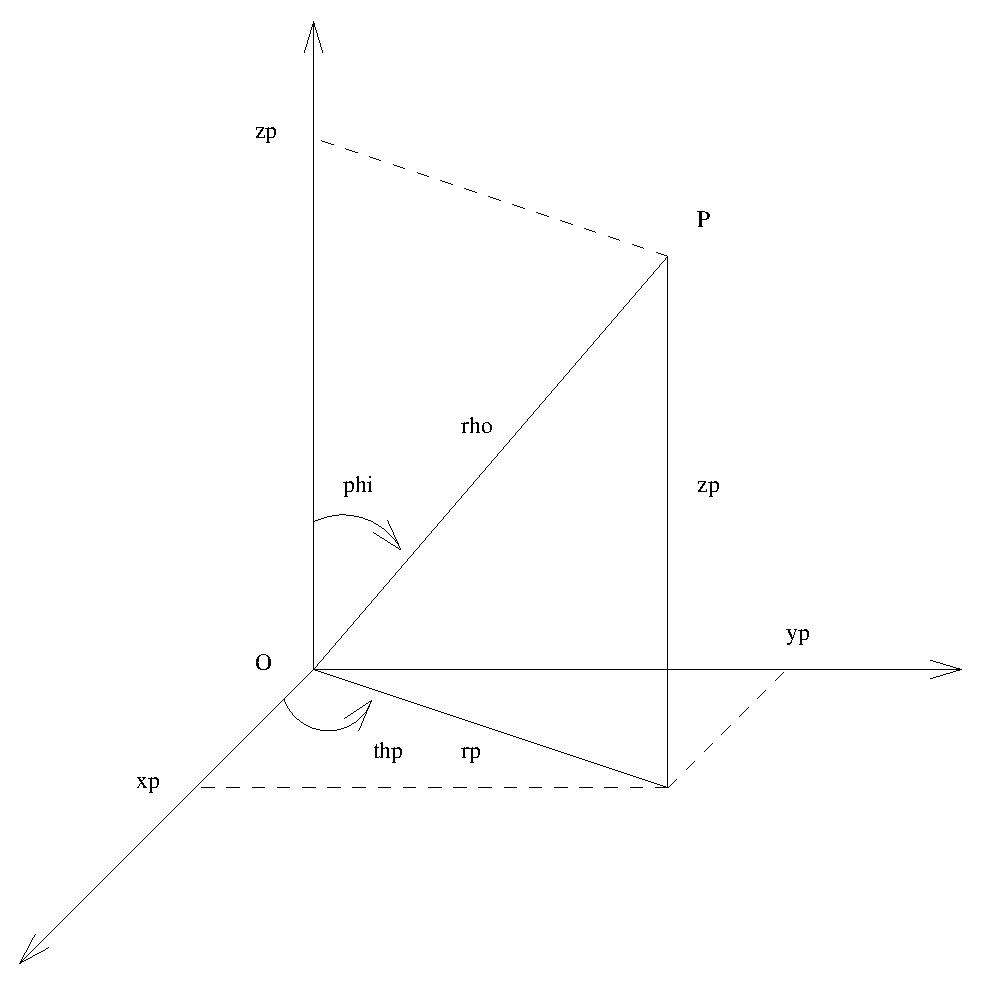
\includegraphics[height=2in]{../../modules/coordinate-systems/pictures/ok-cylindrical-spherical.eps}
%
&
{\parbox{0.4\textwidth}{
Coordinates:
	\begin{itemize}
 	\item $\rho$: distance $|OP|$;
	\item $\phi$: angle $Oz$ to $OP$;
	\item $\theta$: angle $Ox$ to $OP_{xy}$.
	\end{itemize} 

Combination:
\begin{itemize}
    \item Polar in $Oxy$ -- $(r, \theta)$;
    \item Polar in $Ozr$ -- $(\rho, \phi)$.
\end{itemize}

Range of coordinates:
\begin{itemize}
 \item $\rho$:  $[0,\infty)$;
  \item $\phi$:  $[0, \pi]$;
  \item $\theta$:  $[0,2\pi)$.
\end{itemize}
}}
\end{tabular}
  \end{table}

\end{frame}
\begin{frame}
 \frametitle{Transition Spherical - Rectangular coordinates}
\begin{columns}
\column{0.45\textwidth}
\psset{xunit=1cm, yunit=1cm}
\begin{pspicture}(-3,-2)(2,2)
\tiny
\renewcommand{\fcScreen}{[-1 -0.4 -0.25] -1}
\fcAxesIIId{5}{5}{5}
\fcPutIIId[r]{[0 -0.15 0.15]}{$O$}
\fcLineIIId[linestyle=dotted]{[3 0 0]}{[3 3 0]}
\fcLineIIId[linestyle=dotted]{[3 3 0]}{[0 3 0]}
\fcLineIIId[linestyle=dotted]{[0 0 0]}{[0 3 0]}
\fcLineIIId{[0 0 0]}{[3 3 0]}
\fcLineIIId{[3 3 0]}{[3 3 3]}
\fcLineIIId{[0 0 0]}{[3 3 3]}
\fcLineIIId{[0 0 3]}{[3 3 3]}
\fcPutIIId[l]{[3.1 3.1 3.1]}{$P$}
\fcPutIIId[r]{[3 -0.1 0]}{$x_P$}
\fcPutIIId[t]{[3 3 0]}{$Q$}
\fcPutIIId[b]{[0 3.1 0]}{$y_P$}
\fcPutIIId[l]{[1.5 2.5 1.2]}{$z_P$}
\fcPutIIId[r]{[0 0 3]}{$z_P~~$}
\fcPutIIId[r]{[2.1 2.1 2.1]}{$\rho_P$}
\fcPutIIId[rt]{[1 1 1.5]}{$\phi_P~~$}
\fcPutIIId[tr]{[1.8 0.9 0]}{$\theta_P$}
\fcCurveIIId[linecolor=red, arrows=->]{0}{54.74}{ %
t sin 45 cos mul 1.7 mul % 
t sin 45 sin mul 1.7 mul %
t cos 1.7 mul %
} %
\fcCurveIIId[linecolor=red, arrows=->]{0}{45}{ %
t cos 1.7 mul % 
t sin 1.7 mul %
0 %
} %
\end{pspicture} 
\column{0.55\textwidth}


\pause
Spherical to rectangular:\pause
\begin{align*}
 x & = r\cos\theta = \rho\sin\phi \cos\theta \\
  y & = r\sin\theta = \rho\sin\phi \sin\theta \\
  z & = \rho\cos\phi
\end{align*}

\pause
Rectangular to spherical:\pause
$$\rho = \sqrt{x^2+y^2+z^2} \quad , \quad r = \sqrt{x^2+y^2}$$
$$\cos\phi = \frac{z}{\rho} \quad , \quad \sin\phi = \frac{r}{\rho}$$
$$\cos\theta = \frac{x}{r} \quad , \quad \sin\theta = \frac{y}{r}$$
\end{columns}
\end{frame}

\begin{frame}
 \frametitle{Curvilinear boxes}
 
 Polar ``wedge'':
 %
$$C  = \{ P(r,\theta) \; | \;r_0 \leqslant
r \leqslant r_0+\Delta r,  \theta_0 \leqslant \theta
\leqslant \theta_0+\Delta \theta\} \; .$$
%
Shape? \pause Area = ...?
\pause

\bigskip

Cylindrical ``box'':
%
$$X = \{ P(r,\theta, z) \; | \; 0 \leqslant r \leqslant r_0\, ,
0 \leqslant \theta \leqslant \theta_0\, ,
0 \leqslant z \leqslant z_0\}$$

\pause
Shape ? \pause Volume = ...?

\bigskip

\pause
Spherical ``box'':
%
$$Y = \{ P(\rho, \phi, \theta) \; | \; 0 \leqslant \rho \leqslant \rho_0\, ,
0 \leqslant \phi \leqslant \phi_0\, ,
0 \leqslant \theta \leqslant \theta_0\}$$

\pause
Shape? \pause Volume = ...?

\end{frame}
}% end lecture

% begin lecture
\lect{2014}{Lecture  3}{3}{
\section{Vectors}
\begin{frame}
 \frametitle{Vectors}

\begin{itemize}
 \item Location of projector from current position and orientation:

\pause
\begin{itemize}
  \item direction of projector
  \item distance to projector
\end{itemize}

\pause
\item (direction, distance=magnitude) $\Longleftrightarrow$ \textit{vector}

\pause
\item Examples:
\begin{itemize}
  \item Force
  \item Velocity
  \item Displacement
\end{itemize}
\end{itemize}

\end{frame}
\begin{frame}
 \frametitle{Displacement Vectors}

\pause
  Displacement vector = ordered pair of points, $(A,B)$


\begin{itemize}
 \item Represented as an arrow
 \item $A$: tail, $B$: head
 \item Notation: $(A,B) = \overrightarrow{AB} = \textbf{AB}$
  \item Magnitude: $|\textbf{AB}| = |\overrightarrow{AB}|$. 
  \item Direction: Geometric direction from $A$ to $B$, if $A\neq B$ 
  \item If $A=B$:
  \begin{itemize}
    \item Zero magnitude and non-specified direction
    \item $(A,A) = \overrightarrow{AA} = \textbf{AA}$: zero displacement vector.
  \end{itemize}
  \item Displacement vector with tail fixed at $O$:
  \begin{itemize}
    \item Position vector with respect to $O$;
    \item $(O,P) = \overrightarrow{OP} = \textbf{OP} = \textbf{r}_P$.
  \end{itemize}
\end{itemize}

\end{frame}
\begin{frame}
\frametitle{Equality and Equivalence of Displacement Vectors}
\begin{itemize}
\item<1-> We define two displacement vectors to be equal if:
\[ 
\textbf{AB} = \textbf{DC}  \Longleftrightarrow A=D \text{ and } B=C
\]
\item<2-> Equal displacement vectors $\rightarrow$ same magnitude and direction.
\item<3-> Same magnitude and direction $\not\rightarrow$ equal displacement vectors. 

\item<4-> We define two displacement vectors to be \alert<4>{equivalent} if they have the \alert<4>{same magnitude and direction}. We write $\alert<4>{\textbf{AB} \equiv \textbf{DC}}$.
\item 
\[ 
\textbf{AB} \equiv \textbf{DC} \Longleftrightarrow ABCD \text{ is a parallelogram}\;.
\]
\end{itemize}
\end{frame}
\begin{frame}
 \frametitle{Vectors}

  \begin{itemize}
   \item Vector $\textbf{u}$: \\
      set of displacement vectors with given direction and magnitude

    \item  Magnitude of $\textbf{u}$: common given magnitude.

    \item Direction of $\textbf{u}$: common given direction, if non-zero magnitude.

    \item Set of zero displacement vectors = zero vector, $\textbf{0}$. \pause

    \item Representative for $\textbf{u}$: \\
      displacement vector $\textbf{AB}$ with the same direction and magnitude

\begin{figure}[h]
  \psfrag{A}{$A$}
  \psfrag{B}{$B$}
  \psfrag{C}{$C$}
  \psfrag{D}{$D$}
  \psfrag{E}{$E$}
  \psfrag{F}{$F$}
  \psfrag{u}{$\textbf{u}$}
  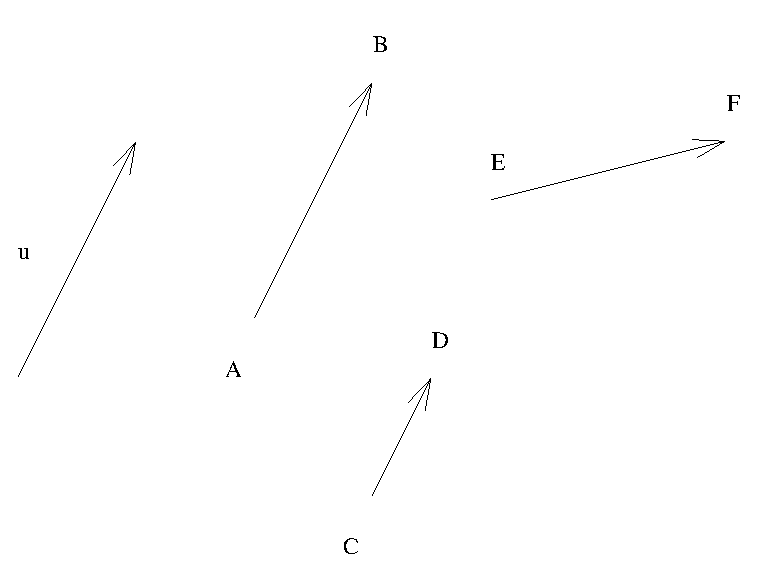
\includegraphics[height=1in]{../../modules/vectors/pictures/ok-vector_representatives.eps}
  \label{fig:vector_representative}

\end{figure}

    \item Intuitive notation:  $\textbf{u}=\textbf{AB}$.

    \item Graphical representation: arrow without fixed tail and head.

    %\item Major advantage: we can translate displacement vectors.
  \end{itemize}
\end{frame}
\begin{frame}
 \frametitle{Addition of Vectors}

  \begin{itemize}
    \item By adding representative displacement vectors: Triangle Rule
\only<2>{
\begin{figure}[h]
  \psfrag{A}{$A$}
  \psfrag{B}{$B$}
  \psfrag{C}{$C$}
  \psfrag{P}{$P$}
  \psfrag{Q}{$Q$}
  \psfrag{R}{$R$}
  \psfrag{u}{$\textbf{u}$}
  \psfrag{v}{$\textbf{v}$}
  \psfrag{uv}{$\textbf{u}+\textbf{v}$}
  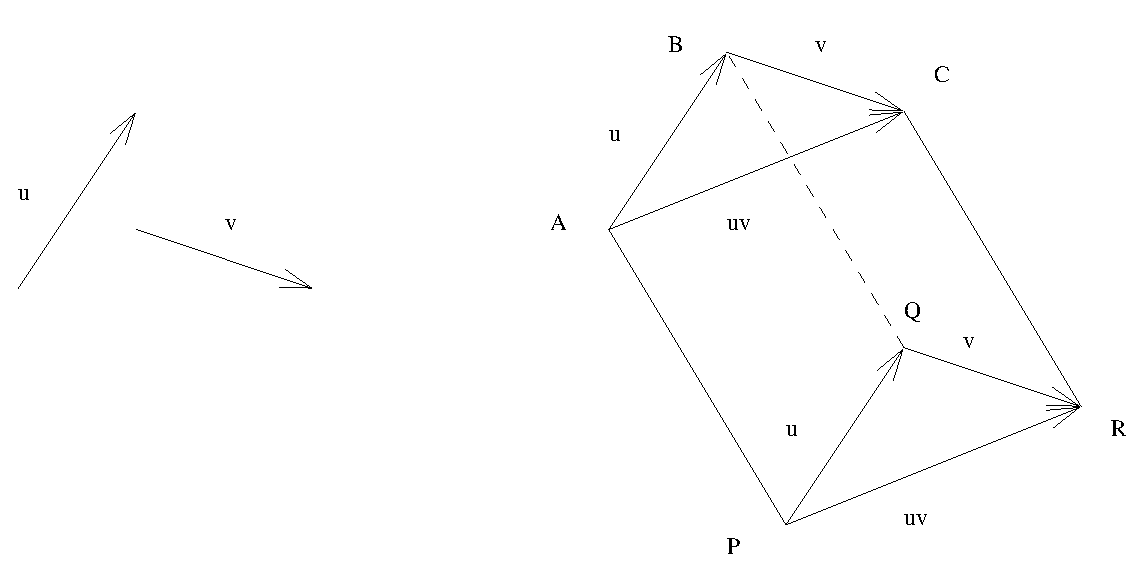
\includegraphics[height=1in]{../../modules/vectors/pictures/ok-vector_addition.eps}
  \label{fig:vector_addition}
  %\caption{Sum of two vectors}
\end{figure}}
    \item<3-> Properties:
    \begin{itemize}
      \item<4-> Commutative, $\textbf{u}+\textbf{v}$ = $\textbf{v}+\textbf{u}$ : Parallelogram Rule
\only<5, 10>{
\begin{figure}[h]
  \psfrag{A}{$A$}
  \psfrag{B}{$B$}
  \psfrag{C}{$C$}
  \psfrag{D}{$D$}
  \psfrag{u}{$\textbf{u}$}
  \psfrag{v}{$\textbf{v}$}
  \includegraphics[height=1in]{../../modules/vectors/pictures/ok-tri-para_rules.eps}
  \label{fig:tripara_rules}
  %\caption{Triangle and Parallelogram Rules}
\end{figure}}

      \item<6-> Associative, $(\textbf{u}+\textbf{v})+\textbf{w} = \textbf{u}+(\textbf{v}+\textbf{w})$ \\
      Extends addition to $\textbf{u}+\textbf{v}+\textbf{w}$
\only<7>{
\begin{figure}[h]
  \psfrag{A}{$A$}
  \psfrag{B}{$B$}
  \psfrag{C}{$C$}
  \psfrag{D}{$D$}
  \psfrag{u}{$\textbf{u}$}
  \psfrag{v}{$\textbf{v}$}
  \psfrag{w}{$\textbf{w}$}
  \psfrag{uv}{$\textbf{u}+\textbf{v}$}
  \psfrag{vw}{$\textbf{v}+\textbf{w}$}
  \psfrag{uvw}{$\textbf{u}+\textbf{v}+\textbf{w}$}
  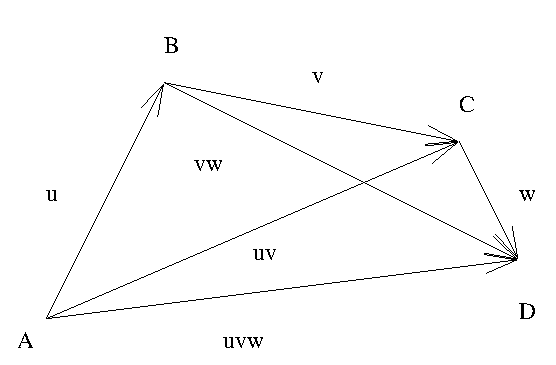
\includegraphics[height=1.5in]{../../modules/vectors/pictures/ok-assoc_addition.eps}
  \label{fig:assoc_adition}
  %\caption{Sum of three vectors}
\end{figure}}

      \item<8-> Opposite vector: If $\textbf{u}=\textbf{AB}$, then $\textbf{AB} + \textbf{BA} = \textbf{0}$,
      hence $\textbf{BA} = -\textbf{u}$.
    \end{itemize}
    \item<9-> Difference of vectors: $\textbf{u}-\textbf{v} = -\textbf{v}+\textbf{u}\textbf{}$: Parallelogram rule.

  \end{itemize}

\end{frame}
\begin{frame}
\frametitle{Linear Combinations}
\begin{columns}
\column{0.3\textwidth}
\psset{xunit=0.6cm, yunit=0.6cm}
\begin{pspicture}(-2,-2)(3,3)
\fcBoundingBox{-2}{-2}{3}{3}
\rput[br](1.9, 2.1){$\bm u$}
\psline[arrows=->](0,0)(3,3)

\uncover<3>{
\psline[arrows=->, linecolor=red](0,0)(1.5,1.5)
\rput[tl](0.75, 0.75){$\alert<3>{\frac{1}{2}\bm u}$}
}

\uncover<4>{
\psline[arrows=->, linecolor=red](0,0)(2,2)
\rput[tl](1, 1){$\alert<4>{\frac{2}{3}\bm u}$}
}
\uncover<5>{
\psline[arrows=->, linecolor=red](0,0)(1,1)
\rput[tl](0.5, 0.5){$\alert<5>{\frac{1}{3}\bm u}$}
}
\uncover<6>{
\psline[arrows=->, linecolor=red](0,0)(-2,-2)
\rput[tl](-1, -1){$\alert<6>{-\frac{1}{2}\bm u}$}
}
\end{pspicture}
\column{0.7\textwidth}
\begin{itemize}
\item<1-> Let $\bm{u}$ be vector, $c$ be a real number (scalar).
\item<2-> Define \alert<2>{the product of the vector $\bm u$ and the scalar $c$} as follows.
\begin{itemize}
\item<2-> If $c >0$ define $c\bm{u}$ as the vector:
\begin{itemize}
\item with the same direction
\item with magnitude proportional with coefficient $c$ to the magnitude of $\bm u$, i.e., $|c\bm{u}| = c|\bm{u}|$.
\end{itemize}

\item<6-> If $c<0$ define $c\bm{u}$ as the vector $(-c)(-\bm{u})$, i.e, as the vector:
\begin{itemize}
\item with opposite direction
\item with magnitude $|c\bm{u}| = |(-c)(-\bm{u})| = (-c)|-\bm{u}| = |c||\bm{u}|$
\end{itemize}
\item<7-> If $c=0$ then define $c\bm u=0\bm{u} = \bm{0}$.
\end{itemize}
\end{itemize}
\end{columns}
\begin{itemize}
\item If $c_1, \ldots , c_n$ are scalars and $\bm{u}_1,\ldots, \bm{u}_n$ are vectors, we say
\[
\bm{v} = c_1\bm{u}_1+ \dotsb + c_n \bm{u}_n
\]
is a \emph{linear combination} of the vectors $\bm u_1,\dots, \bm u_n$.
\end{itemize}
\end{frame}
\begin{frame}
  \frametitle{Decomposition of a vector along given directions}

  Example: Tension induced by given force.

\begin{figure}[h]
  \psfrag{F}{$\textbf{F}$}
  \psfrag{-F}{$-\textbf{F}$}
  \psfrag{F1}{$\textbf{F}_1$}
  \psfrag{F2}{$\textbf{F}_2$}
  \psfrag{T1}{$\textbf{T}_1$}
  \psfrag{T2}{$\textbf{T}_2$}
  \includegraphics[height=2in]{../../modules/vectors/pictures/ok-tension.eps}
  \label{fig:tension}
  %\caption{Decomposition of a vector}
\end{figure}


\end{frame}
\begin{frame}
 \frametitle{Vectors in Coordinates}

  \begin{itemize}
    \item $Oxyz$: fixed rectangular coordinate system
    \item $\textbf{i}$, $\textbf{j}$, $\textbf{k}$: unit vectors in the fundamental directions
  \end{itemize}

If $P(a,b,c)$ is a point, then
\begin{figure}[h]
  \psfrag{a}{$a$}
  \psfrag{b}{$b$}
  \psfrag{c}{$c$}
  \psfrag{x}{$x$}
  \psfrag{y}{$y$}
  \psfrag{z}{$z$}
  \psfrag{ai}{$a \textbf{i}$}
  \psfrag{bj}{$b \textbf{j}$}
  \psfrag{ck}{$c \textbf{k}$}
  \psfrag{i}{$\textbf{i}$}
  \psfrag{j}{$\textbf{j}$}
  \psfrag{k}{$\textbf{k}$}
  \psfrag{P}{$P(a,b,c)$}
  \psfrag{Px}{$P_x(a,0,0)$}
  \psfrag{Py}{$P_y(0,b,0)$}
  \psfrag{Pz}{$P_z(0,0,c)$}
  \psfrag{Pxy}{$P_{xy}(a,b,0)$}
  \psfrag{O}{$O$}
  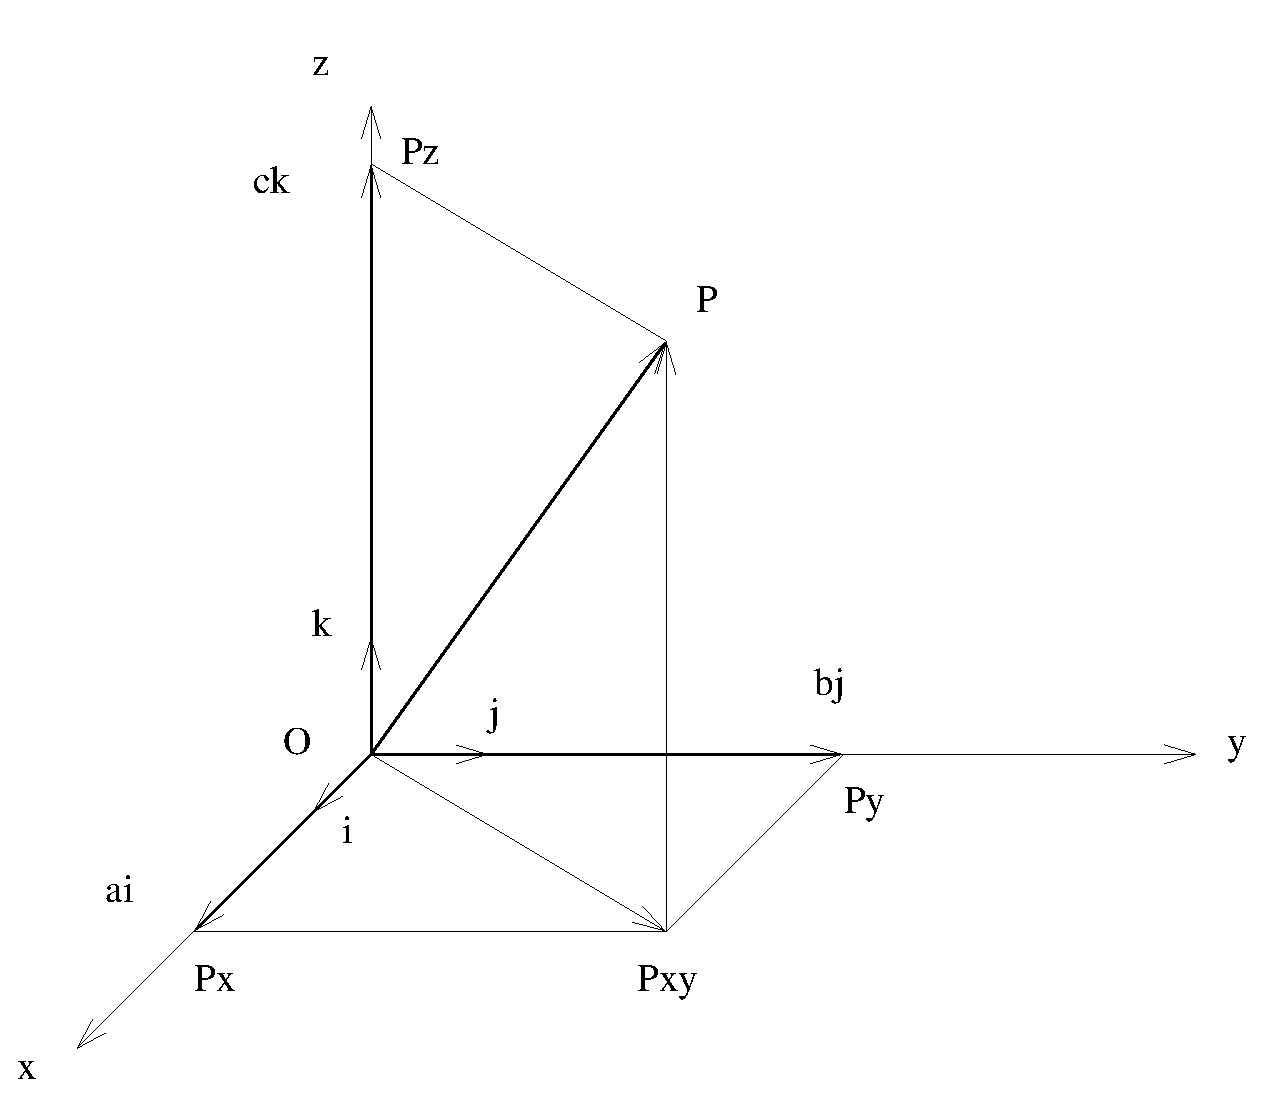
\includegraphics[height=2in]{../../modules/vectors/pictures/ok-vector_decomposition.eps}
  %\caption{Coordinates of a vector}
\end{figure}
%
$$\textbf{OP} = a\textbf{i}+b\textbf{j}+c\textbf{k} = \langle a, b, c\rangle\; .$$

\end{frame}
\begin{frame}
\frametitle{Operations in Coordinates}

\begin{itemize}
 \item Magnitude:
%
$$|\langle a, b, c \rangle| = |OP| = \sqrt{a^2+b^2+c^2}$$
%
\item Addition:
%
$$\langle x_1,y_1,z_1 \rangle + \langle x_2, y_2,z_2\rangle = \langle x_1+x_2, y_1+y_2, z_1+z_2\rangle\; .$$
%
\item Scalar multiple:
%
$$c\langle x, y, z\rangle = \langle cx, cy, cz\rangle\; .$$
%
\item General displacement from $A(x_A, y_A, z_A)$ to $B(x_B, y_B, z_B)$:
%
$$\textbf{AB} = \textbf{AO} +\textbf{OB} = \textbf{OB} - \textbf{OA} = \langle x_B-x_A, y_B-y_A, z_B-z_A\rangle \; .$$
\end{itemize}

\end{frame}
\begin{frame}
 \frametitle{Work done by a constant force}

\only<1>{
\begin{figure}[h]
  \psfrag{F}{$\textbf{F}$}
  \psfrag{O}{$O$}
  \psfrag{P}{$P$}
  \psfrag{a}{$\alpha$}
  \psfrag{pvF}{$\textbf{proj}_{\bm{v}} \textbf{F}$}
  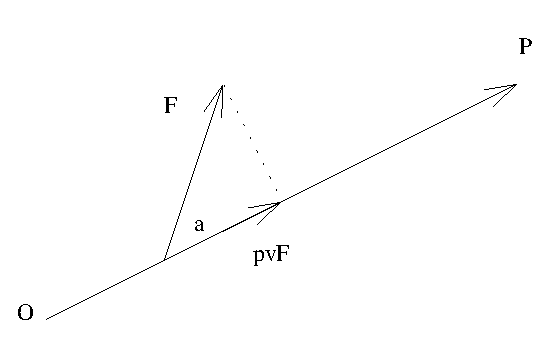
\includegraphics[height=2in]{../../modules/vectors/pictures/ok-positive_work.eps}
\end{figure}

$$W = |\textbf{proj}_{\bm{v}} \textbf{F}| \, |\textbf{OP}| =|\textbf{F}| \, |\textbf{OP}|\, \cos{\alpha}\; .$$
}

\only<2>{
\begin{figure}[h]
  \psfrag{F}{$\textbf{F}$}
  \psfrag{O}{$O$}
  \psfrag{P}{$P$}
  \psfrag{a}{$\alpha$}
  \psfrag{pvF}{$\textbf{proj}_{\bm{v}} \textbf{F}$}
  \includegraphics[height=2in]{../../modules/vectors/pictures/ok-negative_work.eps}
\end{figure}

$$W = - |\textbf{proj}_{\bm{v}} \textbf{F}| \, |\textbf{OP}| = |\textbf{F}| |\textbf{OP}| \cos{\alpha}\; .$$
}

\end{frame}


\begin{frame}
\frametitle{Dot Product}
\begin{columns}
\column{0.5\textwidth}
\begin{pspicture}(-0.5, -0.5)(5,3.2)
\fcBoundingBox{-0.5}{-0.5}{5}{3.2}
\psline[arrows=->](0,0)(4, 2)
\rput[tl](3, 1.5){$\bm v$}
\rput[tl](0.5, 0.2){$\hat{ \bm {v}}$}
\rput[bl](1, 3){$ \bm u$}
\rput[r](-0.5, 1){$\textbf{orth}_{\bm v} \bm u$}

\rput[r](-0.5, 1){$\textbf{orth}_{\bm v} \bm u$}
\rput[tl](1.5, 0.8){$\textbf{proj}_{\bm v} \bm u$}

\psline[arrows=->](0,0)(2,1)
\psline[arrows=->, linecolor=red](0,0)(! 4 20 sqrt div 2 20 sqrt div)

\psline[arrows=->](0,0)(1,3)
\psline[arrows=->](0,0)(! -1 2)
\fcPerpendicular[linestyle=dashed]{[1 3]}{[4 2]}{0.2}%
\fcPerpendicular[linestyle=dashed]{[1 3]}{[-2 4]}{0.2}%
\fcAngle{0.463648}{ 1.249046 }{0.4}{$\alpha$}
\end{pspicture}
\column{0.5\textwidth}

\begin{itemize}
\item<1-> Let $\bm{u}$, $\bm{v}$ vectors, $\bm{v}\neq \bm{0}$.

\item<2-> Let $\textbf{proj}_{\bm{v}} \bm{u}$: projection of $\bm{u}$ along $\bm{v}$.

\item<3-> Let $\textbf{orth}_{\bm{v}} \bm{u}$: projection of $\bm{u}$ orthogonal to $\bm{v}$.

\item<4-> Then $\hat{\bm{v}} = \frac{1}{|\bm{v}|} \bm{v}$ is the unit vector along $\bm{v}$.

\item<5-> Let $\alpha$: angle between $\bm v$ and $\bm u$.

\item<6-> Then $\textbf{proj}_{\bm{v}} \bm{u} =  \cos \alpha |\bm{u}| \hat{\bm{v}}$.

\item<7-> Define dot product of $u$ and $v$:
\[
\bm{u} \cdot \bm{v} =  \cos \alpha |\bm u||\bm{v}| .
\]
\end{itemize}
\end{columns}
\end{frame}

\begin{frame}
\frametitle{The dot Product}
\begin{itemize}
\item<1-> If $\bm{v}=\bm{0}$ or $\bm{u}=\bm{0}$, then $\bm{u}\cdot \bm{v} =0$.
\item<2-> If $\bm{u} \neq \bm 0 \neq \bm{v}$
\[
\bm{u} \cdot \bm{v} = |\bm{u}|  |\bm{v}| \cos{\alpha},
\]
where $\alpha$ is any angle between $\bm u$ and $\bm v$.
\item<3-> If $\bm{u}\neq \bm{0} \neq \bm{v}$, then
$$\bm{u} \cdot \bm{v} = 0 \Longleftrightarrow \bm{u} \bot \bm{v}\; .$$
\item<4-> $\bm{u} \cdot \bm{v} = (\textbf{proj}_{\bm{v}} \bm{u}) \cdot \bm{v}$
\item<5-> The dot product is linear in each argument:
\[
(a \bm{u} + b \bm{w}) \cdot \bm{v} = a \bm{u} \cdot \bm{v} + b \bm{w} \cdot \bm{v}
\]
\[
\bm{u} \cdot (a \bm{v} + b \bm{w}) = a \bm{u} \cdot \bm{v} + b \bm{u} \cdot \bm{w}
\]
\item<6-> Dot product is positive definite:
\[
\begin{array}{l}
\bm{v} \cdot \bm{v} = |\bm{v}|^2 \geqslant 0 \\
\bm{v}\cdot \bm{v} = 0 \Leftrightarrow \bm{v}=\bm{0}
\end{array}
\]
\end{itemize}

\end{frame}
\begin{frame}
\frametitle{Computations in Coordinates}
\begin{itemize}
\item<1-> Let $Oxyz$: rectangular coordinate system
\item<2-> Let $\textbf{i}$, $\textbf{j}$, $\textbf{k}$: unit vectors along axes.
\item<3->
\[ 
\textbf{i} \cdot \textbf{j} = \textbf{j} \cdot \textbf{i} = \textbf{j} \cdot \textbf{k}= \textbf{k} \cdot \textbf{j} = \textbf{i} \cdot \textbf{k} = \textbf{k} \cdot \textbf{i} = 0
\]
\item<4->
\[
\textbf{i} \cdot \textbf{i} = \textbf{j} \cdot \textbf{j} = \textbf{k} \cdot \textbf{k} = 1
\]
\item<5-> 
\begin{theorem}[Can be taken as definition]
\[
\textbf{u} \cdot \textbf{v} = \langle u_1, u_2, u_3 \rangle \cdot \langle v_1, v_2, v_3 \rangle =
u_1v_1 + u_2 v_2 +u_3 v_3\; .
\]
\end{theorem}
 \end{itemize}
\end{frame}

\begin{frame}
\frametitle{Projections in coordinates}
\begin{columns}
\column{0.4\textwidth}
\psset{xunit=0.6cm, yunit=0.6cm}
\begin{pspicture}(-2, -0.5)(5,3.5)
\fcBoundingBox{-2}{-0.5}{5}{3.2}%
\psline[arrows=->](0,0)(4, 2)%
\rput[tl](3, 1.5){$\fcv v$}%
\rput[bl](1, 3){$ \fcv u$}%
\psline[arrows=->, linecolor=blue](0,0)(2,1)%
\rput[tl](1.5, 0.8){$\fcv{proj}_{\fcv v} \fcv u$}%
\psline[arrows=->, linecolor=red](0,0)(! 4 20 sqrt div 2 20 sqrt div)%
\rput[tl](0.5, 0.1){$\widehat{ \fcv {v}}$}%
\psline[arrows=->](0,0)(1,3)%
\fcPerpendicular[linestyle=dashed]{[1 3]}{[4 2]}{0.2}%
\end{pspicture}
\column{0.6\textwidth}
\[
\begin{array}{rcl}
\fcv{u} &=& u_1 \fcv{i} + u_2 \fcv{j} + u_3 \fcv{k} = ( u_1, u_2, u_3 )\\
\fcv{v}&=&v_1 \fcv{i} + v_2 \fcv{j} + v_3 \fcv{k} = ( v_1, v_2, v_3 )
\end{array}
\]
\end{columns}
\uncover<2->{
\begin{theorem}
$\begin{array}{rcl}
\displaystyle\alertNoH{6}{ \text{ comp}_{\fcv v} \fcv u}&\alertNoH{6}{=}& \displaystyle \alertNoH{6}{\frac{\alertNoH{3}{\fcv{u}\cdot \fcv{v}} }{\alertNoH{4}{|\fcv{v}|}}} =\frac{ \alertNoH{3}{ u_1v_1 +u_2v_2+u_3v_3} }{\alertNoH{4}{ \sqrt{v_1^2+v_2^2+v_3^2}}}\\~\\
\displaystyle \alertNoH{5}{{\bf proj}_{\fcv v} \fcv u }&\alertNoH{-1}{=}&\displaystyle \alertNoH{5}{\left(\alertNoH{6}{ \text{comp}_{\fcv v} \fcv{u}}\right) \alertNoH{7}{\widehat{\fcv v}}} = \alertNoH{6}{\frac{\fcv{u}\cdot \fcv{v}}{|\fcv{v}|}} \alertNoH{7}{ \frac{\fcv v}{|\fcv v|}} = \frac{\fcv{u}\cdot \fcv{v}}{\alertNoH{8}{ |\fcv{v}|^2}}\fcv v= \frac{\fcv u \cdot \fcv v}{\alertNoH{8}{ \fcv v\cdot  \fcv v} }\fcv v
\quad .
\end{array}
$
\end{theorem}
}
\end{frame}

\begin{frame}
\frametitle{Angles}
\begin{columns}
\column{0.3\textwidth}
\psset{xunit=0.6cm, yunit=0.6cm}
\begin{pspicture}(-2, -0.5)(5,3.2)
\fcBoundingBox{-2}{-0.5}{5}{3.2}%
\psline[arrows=->](0,0)(4, 2)%
\rput[tl](3, 1.5){$\fcv v$}%
\rput[bl](1, 3){$ \fcv u$}%
\psline[arrows=->, linecolor=blue](0,0)(2,1)%
\psline[arrows=->](0,0)(1,3)%
\fcPerpendicular[linestyle=dashed]{[1 3]}{[4 2]}{0.2}%
\fcAngle{0.463648}{ 1.249046 }{0.4}{$\alpha$}%
\end{pspicture}

Let $\alpha=\angle (\fcv u, \fcv v)$.
\column{0.7\textwidth}
\[
\begin{array}{rcl}
\displaystyle\fcv u \cdot \fcv v& =&\displaystyle |\fcv u||\fcv v|\cos \alpha\\
\uncover<2->{\displaystyle\cos{\alpha} &=&\displaystyle \frac{\textbf{u} \cdot \textbf{v}}{|\textbf{u}|\, |\textbf{v}|} } \\
\uncover<3->{\displaystyle\alpha &=& \displaystyle\arccos{\left( \frac{\textbf{u} \cdot \textbf{v}}{|\textbf{u}|\, |\textbf{v}|} \right)}
}
\end{array}
\]
\end{columns}

\begin{example}
\uncover<4->{
Compute the angle $\angle(( 1,2,3),( 6,5,4))$.}
\uncover<5->{
\[
\begin{array}{rcl}
\alpha &=& \displaystyle \Arccos\left(\frac{(1,2,3) \cdot (6,5,4)}{|(1,2,3) || (6,5,4)|} \right)  \\
&=&\displaystyle \Arccos{\left( \frac{28}{\sqrt{14}\, \sqrt{77}} \right)} = \Arccos{\left( \frac{4}{\sqrt{22}} \right)}
\end{array}
\]
}
\end{example}
\end{frame}

\begin{frame}
 \frametitle{Direction Angles}
\begin{definition}
The direction angles $\alpha, \beta, \gamma$ of the vector $\fcv u$ are defined as the angles between $\fcv u $ and the unit vectors $\fcv i, \fcv j, \fcv k$ (in the same order).
\end{definition}
\begin{columns}
\column{0.5\textwidth}
\psset{xunit=2cm, yunit=2cm}
\begin{pspicture}(-2,-2)(2,2)
\renewcommand{\fcScreen}{[-2 -1 -0.6] 0}
\fcAxesIIId{2}{2}{2}
\fcLineIIId[arrows=->, linecolor=red]{[0 0 0]}{[1.5 1.5 1.5]}
\fcLineIIId[arrows=->, linecolor=blue]{[0 0 0]}{[1 0 0]}
\fcLineIIId[arrows=->, linecolor=blue]{[0 0 0]}{[0 1 0]}
\fcLineIIId[arrows=->, linecolor=blue]{[0 0 0]}{[0 0 1]}
\fcAngleIIId[arrows=->, linecolor=brown]{[1 0 0]}{[1.5 1.5 1.5]}{1}%
\fcAngleIIId[arrows=->, linecolor=brown]{[0 1 0]}{[1.5 1.5 1.5]}{1.4}%
\fcAngleIIId[arrows=->, linecolor=brown]{[0 0 1]}{[1.5 1.5 1.5]}{1.8}%
\fcPutIIId[bl]{[0.75 0 0.25]}{$\alpha~~$}
\fcPutIIId[bl]{[0.75 1.25 0.55]}{$~~\beta$}
\fcPutIIId[r]{[1 1 1.6]}{$~~\gamma$}
\end{pspicture}

\column{0.5\textwidth}

$\textbf{u} = ( u_1, u_2, u_3)$

$\alpha = \angle (\textbf{u},\textbf{i})$

$\beta =
\angle (\textbf{u},\textbf{j})$

$\gamma = \angle (\textbf{u},\textbf{k}) \; .$

$$\cos{\alpha} = \frac{\textbf{u} \cdot \textbf{i}}{|\textbf{u}|\, |\textbf{i}|} =
\frac{u_1}{\sqrt{u_1^2+u_2^2+u_3^2}}$$

Similar for $\cos{\beta}$ and $\cos{\gamma}$. Then:
%
$$\cos^2\alpha + \cos^2\beta + \cos^2\gamma = 1\; .$$
\end{columns}
\end{frame}

\begin{frame}
 \frametitle{Rotational Effect}

 \begin{itemize}
  \item Rigid rod $OP$, fixed at $O$, $\textbf{r}=\textbf{OP}$. Force $\textbf{F}$ applied at $P$.
 \end{itemize}
%
\begin{figure}[h]
  \psfrag{F}{$\textbf{F}$}
  \psfrag{r}{$\textbf{r}$}
  \psfrag{O}{$O$}
  \psfrag{P}{$P$}
  \psfrag{}{$\alpha$}
  \psfrag{pfr}{$\textbf{proj}_{\bm{r}} \textbf{F}$}
  \psfrag{ofr}{$\textbf{orth}_{\bm{r}} \textbf{F}$}
  \includegraphics[height=1.5in]{../../modules/vectors/pictures/ok-torque.eps}
\end{figure}
%
\pause
\begin{itemize}
  \item $\textbf{proj}_{\bm{r}} \textbf{F}$: \pause no effect;
  \item $\textbf{orth}_{\bm{r}} \textbf{F}$: \pause rotational effect:\pause
  \begin{itemize}
    \item Axis of rotation: \pause perpendicular to $\textbf{r}$ and $\textbf{F}$;\pause
    \item Angular velocity: \pause proportional to $|\textbf{orth}_{\bm{r}} \textbf{F}|$;\pause
    \item Linear velocity: \pause proportional to $|\textbf{r}| \, |\textbf{orth}_{\bm{r}} \textbf{F}|$.
  \end{itemize}
\end{itemize}

\end{frame}
\begin{frame}
 \frametitle{Torque}

  Rotation in space $\Longleftrightarrow$ vector\pause
  \begin{itemize}
   \item Axis of rotation $\Longleftrightarrow$ Support of direction \pause
   \item Sense of rotation  $\Longleftrightarrow$ Direction of vector \pause
  \begin{itemize}
      \item Convention: Right Hand Rule\pause
  \end{itemize}
  \item Angular velocity $\Longleftrightarrow$ (proportional to) Magnitude of vector\pause
  \end{itemize}
\begin{center}
 $(\textbf{r}, \textbf{F}) \rightarrow$ rotation $\rightarrow$ vector = torque, $\bm{\tau}$
\end{center}



\begin{itemize}
 \item Support of direction: perpendicular to $\textbf{r}$ and $\textbf{F}$;
 \item Direction: Right Hand Rule;
 \item Magnitude: $|\bm{\tau}| = |\textbf{r}| \, |\textbf{orth}_{\bm{r}} \textbf{F}|$
\end{itemize}

\end{frame}
\begin{frame}
 \frametitle{Cross Product}

\begin{center}
 (\textbf{vector}, \textbf{vector}) $\to$ \textbf{vector}
\end{center}

\begin{figure}[h]
  \psfrag{u}{$\textbf{u}$}
  \psfrag{v}{$\textbf{v}$}
  \psfrag{ovu}{$\textbf{orth}_{\bm{u}} \textbf{v}$}
  \psfrag{a}{$\alpha$}
  \psfrag{uxv}{$\textbf{u} \times \textbf{v}$}
  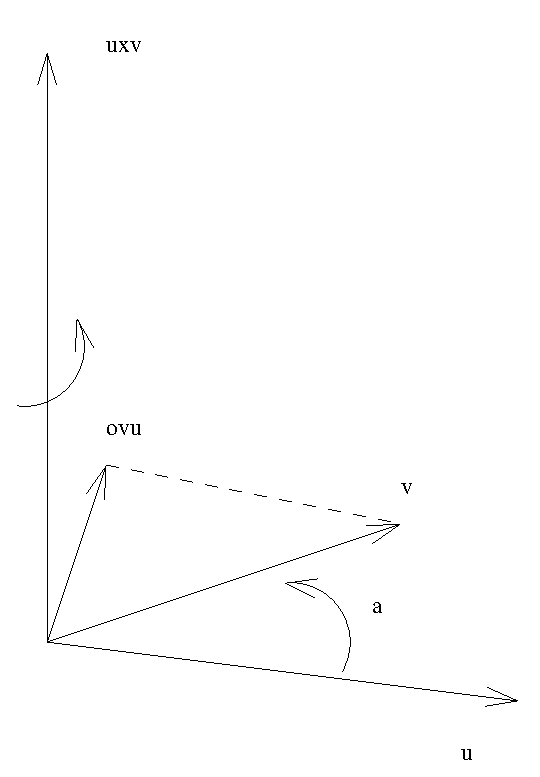
\includegraphics[height=1in]{../../modules/vectors/pictures/ok-cross_product.eps}
\end{figure}

\begin{itemize}
 \item If $\textbf{u}$, $\textbf{v}$ are non-zero and non-collinear vectors:\\
\begin{center}
 $\textbf{u} \times \textbf{v}$ is the vector determined by:
\end{center}
%
\begin{itemize}
 \item Support of direction of $\textbf{u} \times \textbf{v}$:
perpendicular to both $\textbf{u}$ and $\textbf{v}$;
 \item Direction of $\textbf{u} \times \textbf{v}$: given by Right Hand Rule;
 \item Magnitude of $\textbf{u} \times \textbf{v}$: product of $|\textbf{u}|$ and $|\textbf{orth}_{\bm{u}} \textbf{v}|$
%
$$|\textbf{u} \times \textbf{v}| = |\textbf{u}| \, |\textbf{orth}_u \textbf{v}| = |\textbf{u}| |\textbf{v}| \sin{\alpha}$$
%
\end{itemize}
\item If $\textbf{u}=\textbf{0}$ or $\textbf{v}=\textbf{0}$ or
$\textbf{u}$ and $\textbf{v}$ are collinear: \pause $\textbf{u} \times \textbf{v} = \textbf{0} $.
%
\end{itemize}

\end{frame}
\begin{frame}
 \frametitle{Properties of Cross Product}
Let $\textbf{u}$, $\textbf{v}$ non-zero vectors, $\alpha = \angle(\textbf{u},\textbf{v})$.


\begin{itemize}
\item<2-> $|\textbf{v} \times \textbf{u}|  = | \textbf{u} \times \textbf{v}|$.

\uncover<3->{Indeed, that is because $$|\textbf{orth}_{\bm{u}} \textbf{v}| = |\textbf{v}|\sin\alpha
\Longrightarrow |\textbf{u} \times \textbf{v}| = |\textbf{u}| \, |\textbf{v}| \, \sin{\alpha}$$
}

 \item<4-> Cross product is anti-symmetric:
$$\textbf{v} \times \textbf{u} = - \textbf{u} \times \textbf{v} \; .$$
\item<5-> Cross product is linear in each argument:
%
$$ \textbf{u} \times (a\textbf{v} + b\textbf{w}) =
a \textbf{u} \times \textbf{v} + b \textbf{u} \times \textbf{w}$$
%
$$(a\textbf{u} + b\textbf{w}) \times \textbf{v} =
a \textbf{u} \times \textbf{v} + b \textbf{w} \times \textbf{v}$$
\end{itemize}

\end{frame}
\begin{frame}
 \frametitle{Cross Product in Coordinates}

\begin{itemize}
\item Let $\fcv{i}$, $\fcv{j}$, $\fcv{k}$: unit vectors along coordinate axes.
\item We have that
\[ 
\begin{array}{r@{}c@{}cr@{}c@{}cr@{}c@{}c}
\fcv{i} \times \fcv{i} &~=~& \fcv{0}, & \fcv{j} \times \fcv{j} &~=~&\fcv{0} , & \fcv{k} \times \fcv{k} &~=~& \fcv{0} \\
\fcv{i} \times \fcv{j} &~=~& \fcv{k}, & \fcv{j} \times \fcv{k} &~=~& \fcv{i}, &  \fcv{k} \times \fcv{i}& ~=~& \fcv{j}\\
\fcv{j} \times \fcv{i} &~=~& -\fcv{k}, & \fcv{k} \times \fcv{j} &~=~& -\fcv{i},& \fcv{i} \times \fcv{k} &~=~& -\fcv{j}
\end{array}
\]
\item Let $\begin{array}{rclcl}
\fcv{u} &=& u_1 \fcv{i} + u_2 \fcv{j} + u_3 \fcv{k} &=& \langle u_1, u_2, u_3 \rangle \\
\fcv{v}&=&v_1 \fcv{i} + v_2 \fcv{j} + v_3 \fcv{k} &=& \langle v_1, v_2, v_3 \rangle\end{array}$.
\item 
\[\begin{array}{rcl}
\fcv{u} \times \fcv{v} &=& (u_1 \fcv{i} + u_2 \fcv{j} + u_3 \fcv{k})
\times (v_1 \fcv{i} + v_2 \fcv{j} + v_3 \fcv{k})\\
&=& (u_2v_3 -u_3v_2) \fcv{i} + (u_3v_1-u_1v_3) \fcv{j} + (u_1v_2-u_2v_1) \fcv{k} \\
\fcv{u} \times \fcv{v} &=& 
\langle u_1, u_2, u_3 \rangle \times \langle v_1, v_2, v_3 \rangle =
\left|
\begin{array}{ccc}
\fcv{i} & \fcv{j} & \fcv{k} \\
u_1 & u_2 & u_3 \\
v_1 & v_2 & v_3
\end{array}
\right|
\end{array}
\]



\end{itemize}
\end{frame}
\begin{frame}
\[
\fcv{u} \times \fcv{v} = \langle u_1, u_2, u_3 \rangle \times \langle v_1, v_2, v_3 \rangle =
\left|  \begin{array}{ccc}
\fcv{i} & \fcv{j} & \fcv{k} \\
u_1 & u_2 & u_3 \\
v_1 & v_2 & v_3
\end{array}\right|
\]
\begin{example}
Find $\fcv u \times \fcv v$, where $\fcv{u} = \langle 1,2,3\rangle$ and $\fcv{v} = \langle 6,5,4 \rangle$. 
\[
\begin{array}{rcl}
\uncover<2->{%
\fcv{u} \times \fcv{v} &=& \langle 1, 2, 3 \rangle \times \langle 6, 5, 4 \rangle =
\left|  
\begin{array}{ccc}
\fcv{i} & \fcv{j} & \fcv{k} \\
1 & 2 & 3 \\
6 & 5 & 4
\end{array}
\right| \\
} %uncover
\uncover<3->{%
&=& 
\left|\begin{array}{cc}
2 & 3\\
5 & 4
\end{array}\right|\fcv{i} - 
\left| \begin{array}{cc}
1 & 3\\
6 & 4
\end{array}\right| \fcv{j} + 
\left| \begin{array}{cc}
1 & 2\\
6 & 5
\end{array}\right| \fcv{k}  \\~\\
} %uncover
\uncover<4->{%
&=&(2\cdot 4 -3\cdot 5) \fcv{i} - (1\cdot 4 - 3\cdot 6) \fcv{j} + (1 \cdot 5 - 2\cdot 6) \fcv{k} \\~\\
}%uncover
\uncover<5->{%
&=& -7 \fcv{i} + 14 \fcv{j} -7 \fcv{k} =\langle -7, 14, -7\rangle\; .
}
\end{array}
\]
%
\end{example}
\end{frame}
\begin{frame}
\frametitle{Use $\times$ to find vector perpendicular to two given}
Recall $\textbf{u} \times \textbf{v}$ is perpendicular to $\textbf{u}$ and $\textbf{v}$.
\begin{example}
Find a vector perpendicular to $\textbf{u} =(1,1,0) = \textbf{i}+\textbf{j}$ and $\textbf{v}=\textbf{j}+\textbf{k}=( 0,1,1 )$:

\[
\begin{array}{rcl}
 \textbf{w} &= & (\textbf{i}+\textbf{j}) \times (\textbf{j}+\textbf{k}) =
\textbf{i} \times \textbf{j} + \textbf{i} \times \textbf{k} +
\textbf{j} \times \textbf{j} + \textbf{j} \times \textbf{k} = \\
& = & \textbf{k} -\textbf{j}+\textbf{0}+\textbf{i} = \textbf{i} - \textbf{j} + \textbf{k} = (1,-1,1)\; .
\end{array}
\]
\end{example}
\end{frame}

\begin{frame}
\frametitle{Use $\times$ to find area of triangle in space}
\begin{columns}
\column{0.3\textwidth}
\psset{xunit=2cm, yunit=2cm}
\begin{pspicture}(-0.3,-0.1)(1.4,1.4)%
\psline[arrows=->](0,0)(1.2,0)%
\psline[arrows=->](0,0)(0.2,1)%
\psline[arrows=->](1.2,0)(0.2,1)%
\psline(0.2,1)(1.4,1)(1.2,0)%
\rput[t](0,-0.1){$A$}
\rput[tl](1.2,-0.1){$B$}
\rput[bl](1.4,1.1){$D$}
\rput[br](0.2,1.1){$C$}
\uncover<2->{%
\rput[l](0.25,0.5){$\fcv w$}%
\fcPerpendicular{[0.2 1]}{[1 0]}{0.1}%
\psline[arrows=->](0.2,0 )(0.2,1)%
}%
\rput[t](0.5, -0.1){$\fcv u$}
\rput[r](0,0.5){$\fcv v$}
\end{pspicture}
\column{0.7\textwidth}
\begin{itemize}
\item $A$, $B$, $C$ points in space, $\textbf{u} = \textbf{AB}$, $\textbf{v}=\textbf{AC}$.
\item<2-> Then $|\textbf{w}| = |\textbf{orth}_{\bm{u}} \textbf{v}| = \text{ distance from } C \text{ to } AB\; .$
\item<3-> $|\textbf{u} \times \textbf{v}| = |\textbf{orth}_{\bm{u}} \textbf{v}| \, |\textbf{u}| =
2 \text{area}(ABC) = \text{area}(ABDC)$
\item<4-> $|\textbf{u} \times \textbf{v}|$ = Area of parallelogram on sides $\textbf{u}$ and $\textbf{v}$.
\end{itemize}
%
\end{columns}
\end{frame}

\begin{frame}
\begin{example}
\begin{columns}
\column{0.3\textwidth}
\psset{xunit=0.7cm, yunit=0.7cm}
\begin{pspicture}(-0.1, -1)(4,3.5)
\fcBoundingBox{-0.2}{-1}{4}{3.5}
\fcAxesIIId{3}{3}{3}%
\pscustom*[linecolor=cyan]{%
\fcPolyLineIIId{[1 2 3] [2 3 1] [3 1 2] [1 2 3]}
}
\end{pspicture}
\column{0.7\textwidth}

Find the area of the triangle $A(1,2,3)$, $B(2,3,1)$, $C(3,1,2)$.

\end{columns}
\[\begin{array}{rcl}
\displaystyle \text{Area}(ABC) &=&\displaystyle \frac{1}{2}|\textbf{AB} \times \textbf{AC}| =
\frac{1}{2}|( 1,1,-2) \times ( 2, -1, -1) | \\~\\
&=&\displaystyle\frac{1}{2} |( -3, -3, -3 )| \\~\\
&=&\displaystyle \frac{3\sqrt{3}}{2}\; .
\end{array}
\]

\end{example}
\end{frame}

\begin{frame}[label=current]
  \frametitle{Scalar Triple Product}

\begin{itemize}
 \item $A$, $B$, $C$, $D$ points in space;
  \item $\textbf{u} = \textbf{AB}$, $\textbf{v}=\textbf{AC}$, $\textbf{w}=\textbf{AD}$;
  \item $R=R(\textbf{u},\textbf{v},\textbf{w})$: box on sides $\textbf{u}$, $\textbf{v}$, $\textbf{w}$.\pause
%
\begin{figure}[h]
  \psfrag{u}{$\textbf{u}$}
  \psfrag{v}{$\textbf{v}$}
  \psfrag{w}{$\textbf{w}$}
  \psfrag{uxv}{$\textbf{u}\times \textbf{v}$}
  \psfrag{ow}{$\textbf{r}$}
  \includegraphics[height=1in]{../../modules/vectors/pictures/ok-volume_box.eps}
\end{figure}
%
$$\text{Vol}(R) = |\textbf{u} \times \textbf{v}| |\textbf{r}| = |\textbf{u} \times \textbf{v}| \, |\textbf{proj}_{\bm{u} \times \bm{v}} \textbf{w}| =
|\textbf{w} \cdot (\textbf{u} \times \textbf{v})|\; .$$
%
\item $\textbf{w} \cdot (\textbf{u} \times \textbf{v})$: scalar triple product.

\item If $\textbf{u} =\langle u_1,u_2,u_3\rangle$,
$\textbf{v} =\langle v_1,v_2,v_3\rangle$, and $\textbf{w} =\langle w_1,w_2,w_3\rangle$, then
%
$$\textbf{w} \cdot (\textbf{u} \times \textbf{v}) = \left|
\begin{array}{ccc}
w_1 & w_2 & w_3 \\
u_1 & u_2 & u_3 \\
v_1 & v_2 & v_3
\end{array}
 \right|$$
\end{itemize}

\end{frame}
\begin{frame}
  \frametitle{Orientations of Space}

\begin{itemize}
 \item The following are equivalent:
\begin{itemize}
  \item Every vector in space can be decomposed along $\textbf{u}$, $\textbf{v}$, $\textbf{w}$;
  \item The box $R(\textbf{u},\textbf{v},\textbf{w})$ is non-degenerate;
  \item $Vol(R(\textbf{u},\textbf{v},\textbf{w})) \neq 0$;
  \item $\textbf{u} \cdot (\textbf{v} \times \textbf{w}) \neq 0$.
\end{itemize}
%
\item \pause If any of the above is valid: $\{ \textbf{u}, \textbf{v}, \textbf{w}\}$ is a frame.

\item Rectangular coordinate system $\to$ fundamental frame $\{ \textbf{u}, \textbf{v}, \textbf{w}\}$

\item Consistent Right Hand Rule ($\textbf{w}=\textbf{u} \times \textbf{v}$) if and only if
%
$$\textbf{u} \cdot (\textbf{v} \times \textbf{w}) >0$$
%
The frame $\{ \textbf{u}, \textbf{v}, \textbf{w}\}$ is positively oriented if
$\textbf{u} \cdot (\textbf{v} \times \textbf{w}) >0$
%
\end{itemize}

\end{frame}
} %end lecture

% begin lecture
\lect{2014}{Lecture 4}{4}{
\begin{frame}
 \frametitle{Main Questions}


\begin{columns}[t]
\column[T]{0.4\textwidth}

\begin{pspicture}(-1,-2)(3,2)%
\renewcommand{\fcScreen}{[-2 -1 -0.55] 0}%
\tiny%
\fcBoundingBox{-1}{-2}{2}{2}%
\fcStartIIIdScene%
\fcPatchInScene{[2 2 0]}{[1 2 -1]}{[1 2 2]}%
\fcAxesIIIdInScene{2}{2}{2}%
\fcLineIIIdInScene[arrows=->]{[ 0 0 0]}{[1 1 1]}%
\fcLineIIIdInScene{[0.6 0.95 0.35]}{[1.4 1.05 1.65]}%
\fcLineIIIdInScene[arrows=->]{[ 0 0 0]}{[1 2 0.5]}%
\fcFinishIIIdScene[true]%
\fcDotIIId{[1 1 1]}%
\fcDotIIId{[1 2 0.5]}%
\fcPutIIId[lb]{[1 1 1]}{$~~Q(x,y,z)$}%
\fcPutIIId[lb]{[1 2 0.5]}{$~~P(x,y,z)$}%
\end{pspicture}

\column{0.6\textwidth}
What condition(s) should
\begin{itemize}
\item the position vector
\item the coordinates
\end{itemize}

of a point satisfy for it to be on a specific

\begin{itemize}
\item line $L$
\item plane $\mathcal{P}$?
\end{itemize}
\end{columns}

Condition(s) in terms of:
\begin{itemize}
\item position vector $\Rightarrow$ vector (system of) equations;
\item coordinates $\Rightarrow$ scalar equations.
\end{itemize}
\end{frame}

Write vectorial and scalar equations of the line $L$ passing through the given point and with the given direction.

\begin{enumerate}
\item $P_0=(1,2,3)$, $\fcv u= (-3,-2,-1)$.

\answer{
$L: (1,2,3)+ t (-3, -2, -1) $
$L:\left|\begin{array}{rcl}
x&=& 1-3t\\
y&=& 2- 2t\\
z&=& 3-t
\end{array}\right., t\in \mathbb R$
}


\item $P_0=(3,5,7)$, $\fcv u=(2,3,4)$.

\answer{
$L: (3,5,7)+ t (2,3,4) $
$L:\left|\begin{array}{rcl}
x&=& 3+2t\\
y&=& 5+ 3t\\
z&=& 7+4t
\end{array}\right., t\in \mathbb R$
}
\end{enumerate}

\begin{frame}
 \frametitle{Line from Two Points}

\begin{columns}

\column{0.4\textwidth}
\psset{xunit=1.4cm, yunit=1.4cm}
\begin{pspicture}(-1,-0.4)(2.7,2.1)
\fcBoundingBox{-0.8}{-0.4}{4}{2.1}
\renewcommand{\fcScreen}{[-3 -1 -0.2] 0}
\tiny
\uncover<5->{\fcAxesIIId{2}{2}{2}}
\fcLineIIId{[0.5 0.5 1]}{[3 3 0.5]}
\fcLineIIId{[0.5 0.5 1]}{[4 4 0.3]}
\fcLineIIId[arrows=->]{[0 0 0]}{[1 1 0.9]}
\fcPutIIId[br]{[0.5 0.5 0.45]}{$\fcv r_0~$}

\fcLineIIId[linecolor=blue, arrows=->]{[1 1 0.9]}{[2.5 2.5 0.6]}
\fcPutIIId[br]{[1.75 1.75 0.8]}{$\fcv u$}

\fcLineIIId[arrows=->]{[0 0 0]}{[2.5 2.5 0.6]}
\fcPutIIId[b]{[1.25 1.25 0.3]}{$\fcv r_1$}

\fcDotIIId{[1 1 0.9]}
\fcPutIIId[lb]{[1 1 0.95]}{$P_0\uncover<5->{(x_0,y_0, z_0)} $}
\fcDotIIId{[2.5 2.5 0.6]}
\fcPutIIId[lb]{[2.5 2.5 0.65]}{$P_1\uncover<5->{(x_1, y_1, z_1)}$}
\fcDotIIId{[3.5 3.5 0.4]}
\fcLineIIId[arrows=->]{[0 0 0]}{[3.5 3.5 0.4]}
\fcPutIIId[b]{[1.75 1.75 0.2]}{$\fcv r$}
\fcPutIIId[b]{[3.5 3.5 0.5]}{$~P(x,y,z)$}
\fcPutIIId[t]{[4 4 0.3]}{$~L$}
\fcPutIIId[r]{[0 0 0.1]}{$O~~$}
\end{pspicture}
\column{0.6\textwidth}
\begin{itemize}
\item Given: distinct points $P_0$ and $P_1$, position vectors $\textbf{r}_0$ and $\textbf{r}_1$.
\item Goal: write equations of line $L$ through $P_0$ and $P_1$.
\item<2-> Direction of $L$: $\textbf{u} = \textbf{r}_1 - \textbf{r}_0$.
\item<5-> $\fcv{u} = ( x_1-x_0,y_1-y_0,z_1-z_0)$.
\end{itemize}
\end{columns}
\uncover<3->{
\begin{definition}
\alert<1->{Parametric equation} of a line $L$:\\
$
\textbf{r} = \textbf{r}_0 + t(\textbf{r}_1-\textbf{r}_0)
\quad \Leftrightarrow \quad   \textbf{r} = (1-t)\textbf{r}_0 + t\textbf{r}_1
$

\uncover<5->{
\alert<1->{Parametric scalar equations} of a line $L$:
$\left|
\begin{array}{ll}
x & = x_0 + t(x_1-x_0) \\
y & = y_0 + t(y_1-y_0) \\
z & = z_0 + t(z_1-z_0)
\end{array}
\right. \Leftrightarrow \left| \begin{array}{ll}
x & = (1-t)x_0 + tx_1 \\
y & = (1-t)y_0 + ty_1 \\
z & = (1-t)z_0 + tz_1
\end{array}
\right. , \quad t \text{ real number.}$
} %uncover
\end{definition}
} %uncover
\end{frame}

\begin{frame}
 \frametitle{Plane from Point and Normal}

\begin{columns}
  \column{6cm}
\begin{itemize}
 \item<1-> Point $P_0$, with position vector $\textbf{r}_0$;\\
 \uncover<5->{$\textbf{r}_0 = \langle x_0,y_0,z_0\rangle$}
\item<1-> Direction $\textbf{n}$, non-zero vector.\\
  \uncover<5->{$\textbf{n} = \langle a,b,c\rangle$}
\end{itemize}
  \column{6cm}
$\mathcal{P}$: plane\\
passing through $P_0$ and \\
normal to direction $\textbf{n}$.
\end{columns}

\bigskip

\begin{columns}
  \column{6cm}
\begin{center}
 \uncover<2-4>{A point $P(\textbf{r})$ is on $\mathcal{P}$ $\longleftrightarrow$\\}
 \uncover<5->{A point $P(x,y,z)$ is on $\mathcal{P}$ $\longleftrightarrow$\\}
 \uncover<3-4>{\medskip $\textbf{P}_0\textbf{P}$ is normal to $\textbf{n}$ $\longleftrightarrow$\\}
 \uncover<4->{\medskip \textcolor[rgb]{0.98,0.00,0.00}{Implicit vectorial equation}: \\
 $\boxed{ (\textbf{r}-\textbf{r}_0) \cdot \textbf{n} = 0 \;.}$\\}
 \uncover<6->{\medskip\textcolor[rgb]{0.98,0.00,0.00}{Implicit scalar equation}: \\
 $\langle x-x_0, y-y_0, z-z_0\rangle \cdot \langle a,b,c\rangle = 0$\\
 $\boxed{a(x-x_0) + b(y-y_0)+c(z-z_0) = 0}$}
\end{center}

  \column{6cm}
    \only<2-4>{\begin{figure}
        \psfrag{O}{$O$}
        \psfrag{Pi}{$\mathcal{P}$}
        \psfrag{P}{$P$}
        \psfrag{P0}{$P_0$}
        \psfrag{r}{$\textbf{r}$}
        \psfrag{n}{$\textbf{n}$}
        \psfrag{r0}{$\textbf{r}_0$}
        \includegraphics[height=1.5in]{../../modules/vectors/pictures/ok-plane_point_normal_vector.eps}
    \end{figure}}
    \only<5->{\begin{figure}
        \psfrag{O}{$O$}
        \psfrag{x}{$x$}
        \psfrag{y}{$y$}
        \psfrag{z}{$z$}
        \psfrag{Pi}{$\mathcal{P}$}
        \psfrag{P}{$P(x,y,z)$}
        \psfrag{P0}{$P_0(x_0,y_0,z_0)$}
        \psfrag{r}{$\textbf{r}$}
        \psfrag{n}{$\textbf{n}=\langle a,b,c \rangle$}
        \psfrag{r0}{$\textbf{r}_0$}
        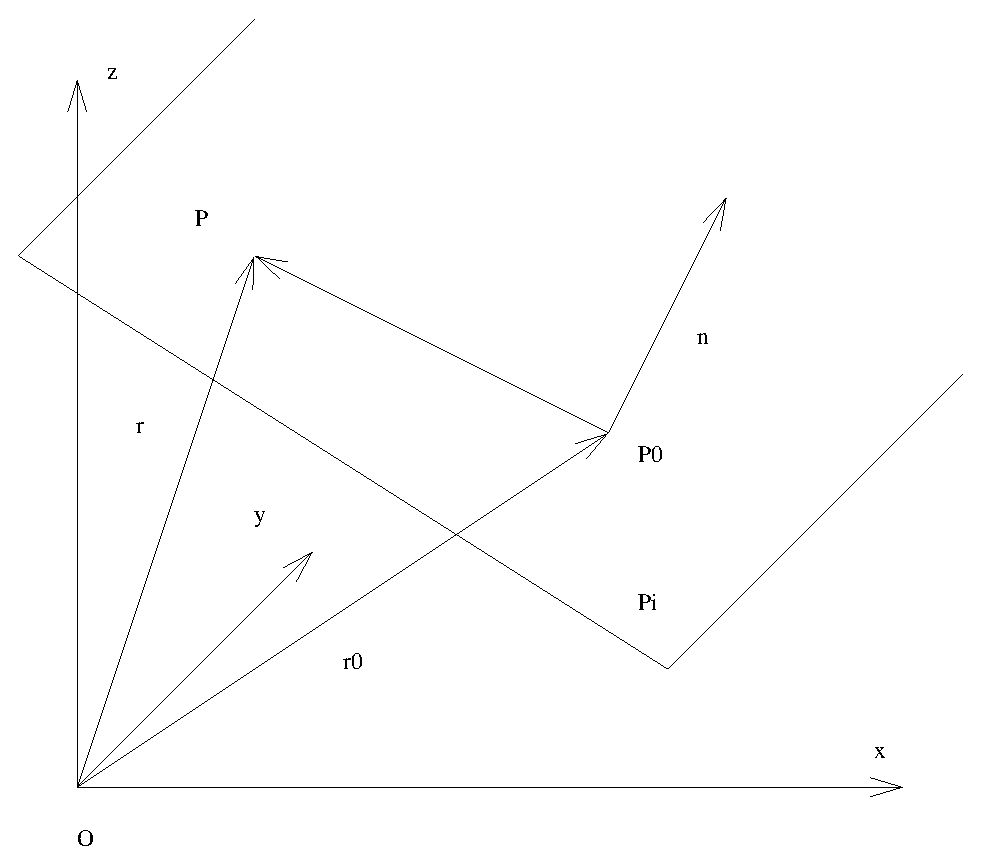
\includegraphics[height=1.5in]{../../modules/vectors/pictures/ok-plane_point_normal_scalar.eps}
    \end{figure}}
\end{columns}
\end{frame}



\begin{frame}
 \frametitle{Example}

Equation of the plane
\begin{itemize}
 \item Passing through $P_0(1,2,3)$;
\item Normal to the direction $\textbf{n} = \langle 6,5,4\rangle$:
\end{itemize}
%
\pause
$$6(x-1) + 5(y-2) + 4(z-3) = 0$$
%
$$6x +5y+4z = 28$$

\pause General equation of a plane:
%
$$ax+by+cz = d$$
%
Coefficients $a,b,c$: \pause components of normal to the plane,
%
$$\textbf{n} = \langle a,b,c\rangle\; .$$

\end{frame}
\begin{frame}
 \frametitle{Plane from Point and two Directions}

\begin{columns}
\column{0.45\textwidth}
\begin{pspicture}(-0.3,-1)(2,2)
\tiny
\renewcommand{\fcScreen}{[-4 -1 -0.4] 0}
\fcParallelogramIIId{[0.1 -1.9 1.36]}{[3.1 1.1 0.16]}{[-3.2 0.8 1.48]}
\fcAxesIIId{2}{2}{2}
%normal: (0.2 0.2 1)
\fcLineIIId[arrows=->, linecolor=blue]{[1 3 -1]}{ [1.6 3.6 -1.24]}
\fcPutIIId[rt]{[1.3 3.3 -1.12]}{$\fcv u$}
\fcLineIIId[arrows=->, linecolor=brown]{[1 3 -1]}{[0.45 3.45 -0.98]}
\fcPutIIId[b]{[0.725 3.225 -0.99]}{$\fcv v ~$}

\fcLineIIId[arrows=->, linecolor=red]{[1 3 -1]}{[1.24 3.24 0.2]}
\fcPutIIId[l]{[1.12 3.12 -0.4]}{$\fcv u \times \fcv v $}

\fcLineIIId[linewidth=0.3pt, linecolor=gray]{[0.43 -0.17 0.948]}{[-1.55 1.45 1.02]}
\fcLineIIId[linewidth=0.3pt, linecolor=gray]{[-0.2 -0.2 1.08]}{[1.6 1.6 0.36]}



\fcLineIIId[arrows=->, linecolor=red]{[0.1 0.1 0.96]}{[0.34 0.34 2.16]}
\fcLineIIId[arrows=->]{[0.1 0.1 0.96]}{[1.3 1.3 0.48]}
\fcPutIIId[tr]{[1.2 1.2 0.5]}{$s\fcv u~~$}
\fcLineIIId[arrows=->]{[0.1 0.1 0.96]}{[-1 1 1]}
\fcPutIIId[b]{[-0.8 0.9 1.1]}{$t\fcv v$}
\fcLineIIId[arrows=->, linecolor=blue]{[0.1 0.1 0.96]}{[0.7 0.7 0.72]}
\fcPutIIId[rt]{[0.4 0.4 0.84]}{$\fcv u$}
\fcLineIIId[arrows=->, linecolor=brown]{[0.1 0.1 0.96]}{[-0.45 0.55 0.98]}
\fcPutIIId[b]{[-0.175 0.325 0.97]}{$\fcv v$}


\fcLineIIId{[-1 1 1]}{ [0.2 2.2 0.52]}%
\fcLineIIId{[1.3 1.3 0.48]}{[0.2 2.2 0.52]}
\fcLineIIId[arrows=->]{[0.1 0.1 0.96]}{[0.2 2.2 0.52]}

\fcLineIIId[arrows=->]{[0 0 0]}{[0.1 0.1 0.96]}
\fcPutIIId[l]{[0.05 0.05 0.48]}{$~\fcv r_0$}

\fcLineIIId[arrows=->]{[0 0 0]}{[0.2 2.2 0.52]}
\fcPutIIId[l]{[0.1 1.1 0.26]}{$~\fcv r_0$}


\fcPutIIId[br]{[0.1 0.1 0.96]}{$P_0~~$}
\end{pspicture}
\column{0.55\textwidth}
\begin{itemize}
\item Given: point $P_0$ with position vector $\textbf{r}_0$. \item Non-parallel directions $\textbf{u}$ and $\textbf{v}$.
\item Goal: give equations of plane $\mathcal P$ through $P_0$ and parallel to both $\textbf{u}$ and $\textbf{v}$.
\end{itemize}
\end{columns}
\only<2>{Normal direction $\textbf{n} = \textbf{u} \times \textbf{v} \neq \textbf{0}$ 

\alert<1->{Implicit vectorial equation}: $P(\textbf{r}) \text{ is on } \mathcal{P} \Longleftrightarrow (\textbf{r}-\textbf{r}_0) \cdot \textbf{n} = 0$

Interpretation:$$\text{Vol}(R(\textbf{r} - \textbf{r}_0,\textbf{u},\textbf{v})) = 0$$}
  
\only<3>{$P(\textbf{r})$ is on the plane $\mathcal{P}$ $\leftrightarrow$

$\textbf{P}_0\textbf{P}$ is a combination of $\textbf{u}$, $\textbf{v}$ $\leftrightarrow$

There are scalars $s$, $t$ such that $\textbf{r}-\textbf{r}_0= s\textbf{u} + t\textbf{v} \leftrightarrow $

\alert<1->{Parametric vectorial equation}: $$\boxed{ \textbf{r} = \textbf{r}_0 + s\textbf{u} + t\textbf{v} \; }$$ for some parameters $s$ and $t$}
\only<4>{
\alert<1->{Parametric vectorial equation}: $$\textbf{r} = \textbf{r}_0 + s\textbf{u} + t\textbf{v}$$ $P_0(x_0,y_0,z_0)$, $P(x,y,z)$ $\textbf{u} = \langle u_1,u_2,u_3\rangle$, $\textbf{v}=\langle v_1,v_2,v_3\rangle$
\alert<1->{Parametric scalar equations}:
$$\left|\begin{array}{ll}
x = & x_0 + su_1+tv_1 \\
y = & y_0 + su_2+tv_2 \\
z = & z_0 + su_3+tv_3
\end{array}
\right.$$ for  $s$, $t$  real parameters.
}
\vskip 10cm
\end{frame}


\begin{frame}
 \frametitle{Example}

$P_0(1,2,3)$, $\textbf{u}=\langle -1,0,2\rangle$, $\textbf{v} = \langle 0,-2,1\rangle$.\pause
%
$$\textbf{n} = \textbf{u} \times \textbf{v} = \left| \begin{array}{ccc}
                           \textbf{i} & \textbf{j} & \textbf{k} \\
			   -1 & 0 & 2 \\
                           0 & -2 & 1
                          \end{array}
\right| = 4\textbf{i}+\textbf{j} +2\textbf{k}$$
%
$$4(x-1)+1(y-2) + 2(z-3) = 0 \Longleftrightarrow 4x+y+2z = 12$$
%
\pause Implicit scalar equation:
%
$$4x+y+2z = 12\; .$$

\pause Parametric vectorial equation:
%
$$\langle x, y, z \rangle = \langle 1,2,3\rangle + s\langle -1, 0, 2\rangle + t\langle 0,-2,1\rangle$$

\pause Parametric scalar equations:
%
$$\left\{ \begin{array}{ll}
           x & = 1 -s \\
           y & = 2-2t \\
           z & = 3 +2s +t
          \end{array}
\right. \quad s,t \text{ real parameters}.$$
%
\end{frame}

\begin{frame}
 \frametitle{Plane from Three Points}

\begin{columns}
\column{0.4\textwidth}
        \psfrag{O}{$O$}
        \psfrag{Pi}{$\mathcal{P}$}
        \psfrag{P}{$P$}
        \psfrag{P0}{$P_0$}
        \psfrag{P1}{$P_1$}
        \psfrag{P2}{$P_2$}
        \psfrag{r}{$\fcv{r}$}
        \psfrag{r0}{$\fcv{r}_0$}
        \psfrag{r1}{$\fcv{r}_1$}
        \psfrag{r2}{$\fcv{r}_2$}
        \psfrag{n}{$\fcv{n}$}
        \psfrag{u}{$\fcv{u}$}
        \psfrag{v}{$\fcv{v}$}
        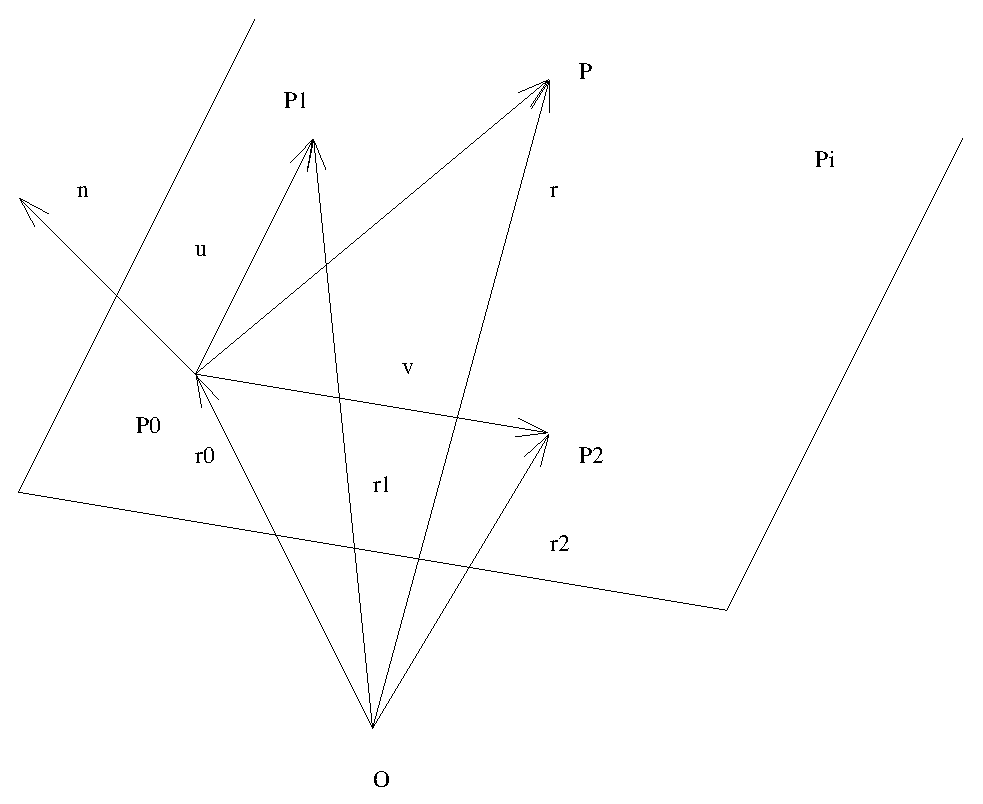
\includegraphics[height=1.5in]{../../modules/vectors/pictures/ok-plane_three_points.eps}
\column{0.6\textwidth}
\begin{itemize}
\item Given: three non-collinear points $P_0(\fcv{r}_0)$, $P_1(\fcv{r}_1)$, $P_2(\fcv{r}_2)$.
\item Goal: find equations fo plane $\mathcal{P}$ passing through $P_0$, $P_1$, and $P_2$.
\end{itemize}
\end{columns}
\only<2>{
The plane is parallel to $\fcv{u} = \fcv{P}_0\fcv{P}_1 = \fcv{r}_1 -\fcv{r}_0$ and passing through $P_0$ $\Rightarrow$ this problem was solved previously.

Normal $\fcv{n} = \fcv{u} \times \fcv{v} =
(\fcv{r}_1-\fcv{r}_0) \times (\fcv{r}_2-\fcv{r}_0)$  \\

\alert<1->{Implicit vectorial equation}:
  $$(\fcv{r}-\fcv{r}_0) \cdot \fcv{n} = 0$$
  %
  $$\boxed{(\fcv{r}-\fcv{r}_0) \cdot [(\fcv{r}_1-\fcv{r}_0) \times (\fcv{r}_2-\fcv{r}_0)] = 0}$$
%
$$\text{Vol}(R(\fcv{P}_0\fcv{P}, \fcv{P}_0\fcv{P}_1, \fcv{P}_0\fcv{P}_2)) = 0$$
  }

 \only<3>{
 \alert<1->{Implicit vectorial equation}: $(\fcv{r}-\fcv{r}_0) \cdot [(\fcv{r}_1-\fcv{r}_0) \times (\fcv{r}_2-\fcv{r}_0)] = 0$

Let the points have coordinates $P_0(x_0,y_0,z_0)$, $P_1(x_1,y_1,z_1)$, $P_2(x_2,y_2,z_2)$. $P(x,y,z)$ is on plane $\mathcal{P}$:\\

\alert<1->{Implicit scalar equation}:
%
$\left| \begin{array}{ccc}
          x-x_0 & y-y_0 & z-z_0 \\
          x_1-x_0 & y_1-y_0 & z_1-z_0 \\
          x_2-x_0 & y_2-y_0 & z_2-z_0	
         \end{array}
\right| = 0\; .$
%
  }
\end{frame}


\begin{frame}
 \frametitle{Main Questions}

\begin{itemize}
  \item Geometric objects:
  \begin{itemize}
    \item Points: $P(\textbf{r})$.
    \item Lines: $L$: $\textbf{r}= \textbf{r}_0 + t\textbf{u}$
    \item Planes: $\mathcal{P}$: $(\textbf{r}-\textbf{r}_0)\cdot \textbf{n} =0$
  \end{itemize}

  \item Relationships/Geometric Quantities:
  \begin{itemize}
      \item Parallelism
      \item Perpendicularity
      \item Angles
      \item Distances
      \item Intersections
  \end{itemize}
\end{itemize}
\end{frame}
\begin{frame}
\frametitle{Point and line}

\begin{columns}
\column{0.4\textwidth}
        \psfrag{L}{$L$}
        \psfrag{P}{$P(\fcv{r}_1)$}
        \psfrag{P0}{$P_0(\fcv{r}_0)$}
        \psfrag{u}{$\fcv{u}$}
        \psfrag{r12}{$\fcv{r}_1-\fcv{r}_0$}
        \psfrag{orth}{$\fcv{\fcv{orth}}_{\fcv{u}}(\fcv{r}_1-\fcv{r}_0)$}
        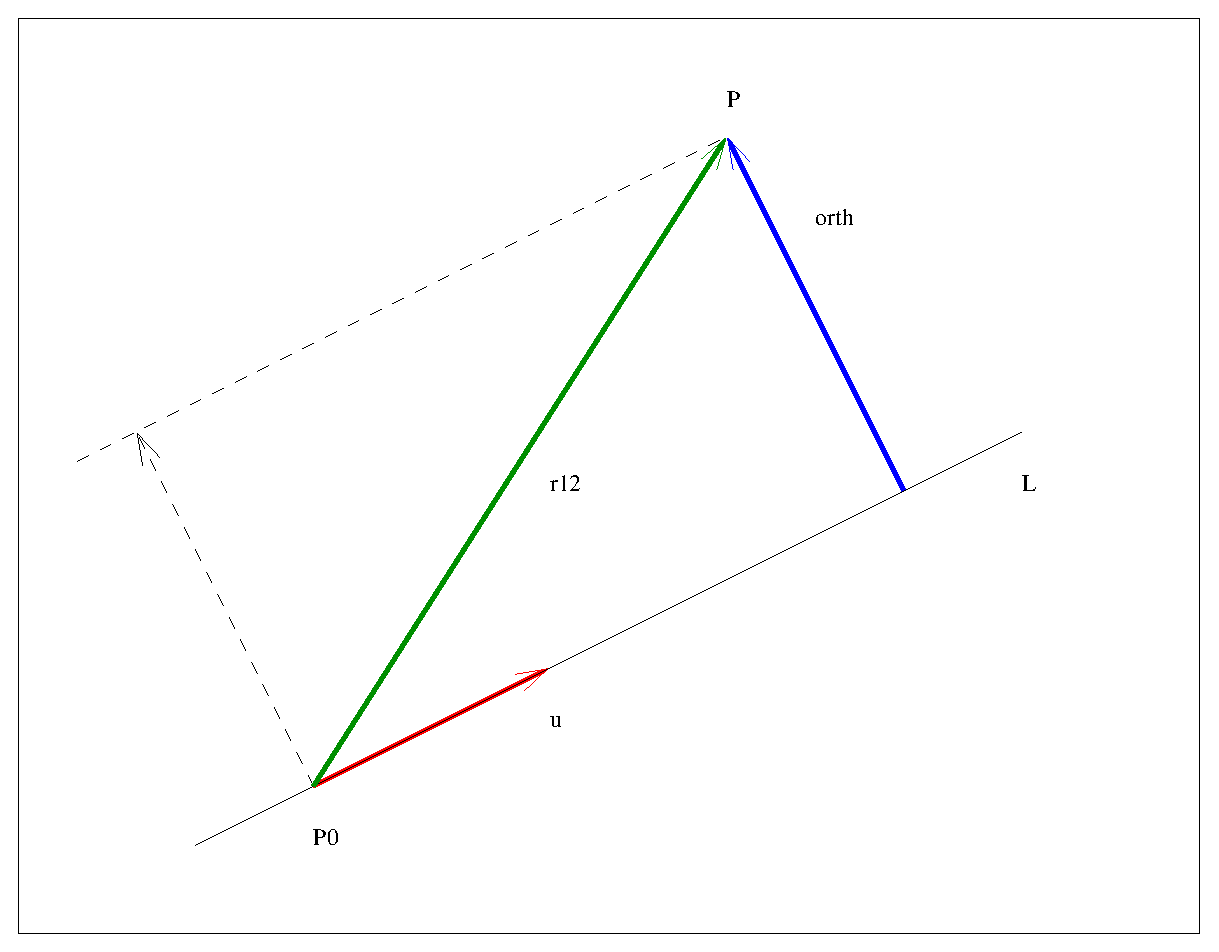
\includegraphics[height=1.3in]{../../modules/vectors/pictures/ok-distance_point_line.eps}
\column{0.6\textwidth}
\begin{itemize}
\item Given: Point $P(\fcv{r}_1)$, 
\item line $L: \quad \fcv{r}=\fcv{r}_0+t\fcv{u}$.
\item Goal: find the distance between $P$ and $L$.
\end{itemize}

\alert<1->{Distance} from $P$ to $L$:
\uncover<2->{
$$d(P,L) = |\fcv{\text{orth}}_{\bm{u}}(\fcv{r}_1-\fcv{r}_0)|$$
$$\boxed{d(P,L) = \frac{|(\fcv{r}_1-\fcv{r}_0) \times \fcv{u}|}{|\fcv{u}|}}$$}

\end{columns}
\end{frame}
\begin{frame}
  \frametitle{Point and plane}
  Point $P(\textbf{r}_1)$ \hspace{2cm} Plane $\mathcal{P}: \quad (\textbf{r}-\textbf{r}_0)\cdot \textbf{n} = 0$
\bigskip
  \begin{columns}
  \column{6cm}
  \textcolor[rgb]{0.98,0.00,0.00}{Distance} from $P$ to $\mathcal{P}$:
  \uncover<2->{
  $$d(P,\mathcal{P}) = |\textbf{\text{proj}}_{\bm{n}}(\textbf{r}_1-\textbf{r}_0)|$$
  $$d(P,\mathcal{P}) = \frac{|(\textbf{r}_1-\textbf{r}_0) \cdot \textbf{n}|}{|\textbf{n}|}$$}
  %
  \uncover<3->{
  \textcolor[rgb]{0.98,0.00,0.00}{Scalar equation}:
  $P(x_1,y_1,z_1)$
   $$\mathcal{P}: ax+by+cz+d=0$$}
   \uncover<4->{$$\textbf{n} = \langle a,b,c\rangle$$
   $$\boxed{\text{Distance} = \frac{|ax_1+by_1+cz_1+d|}{\sqrt{a^2+b^2+c^2}}}$$}
  \column{6.5cm}
      \begin{figure}
        \psfrag{cP}{$\mathcal{P}$}
        \psfrag{P}{$P(\textbf{r}_1)$}
        \psfrag{P0}{$P_0(\textbf{r}_0)$}
        \psfrag{n}{$\textbf{n}$}
        \psfrag{r12}{$\textbf{r}_1\!-\!\textbf{r}_0$}
        \psfrag{proj}{$\textbf{\text{proj}}_{\bm{n}}(\textbf{r}_1\!-\!\textbf{r}_0)$}
        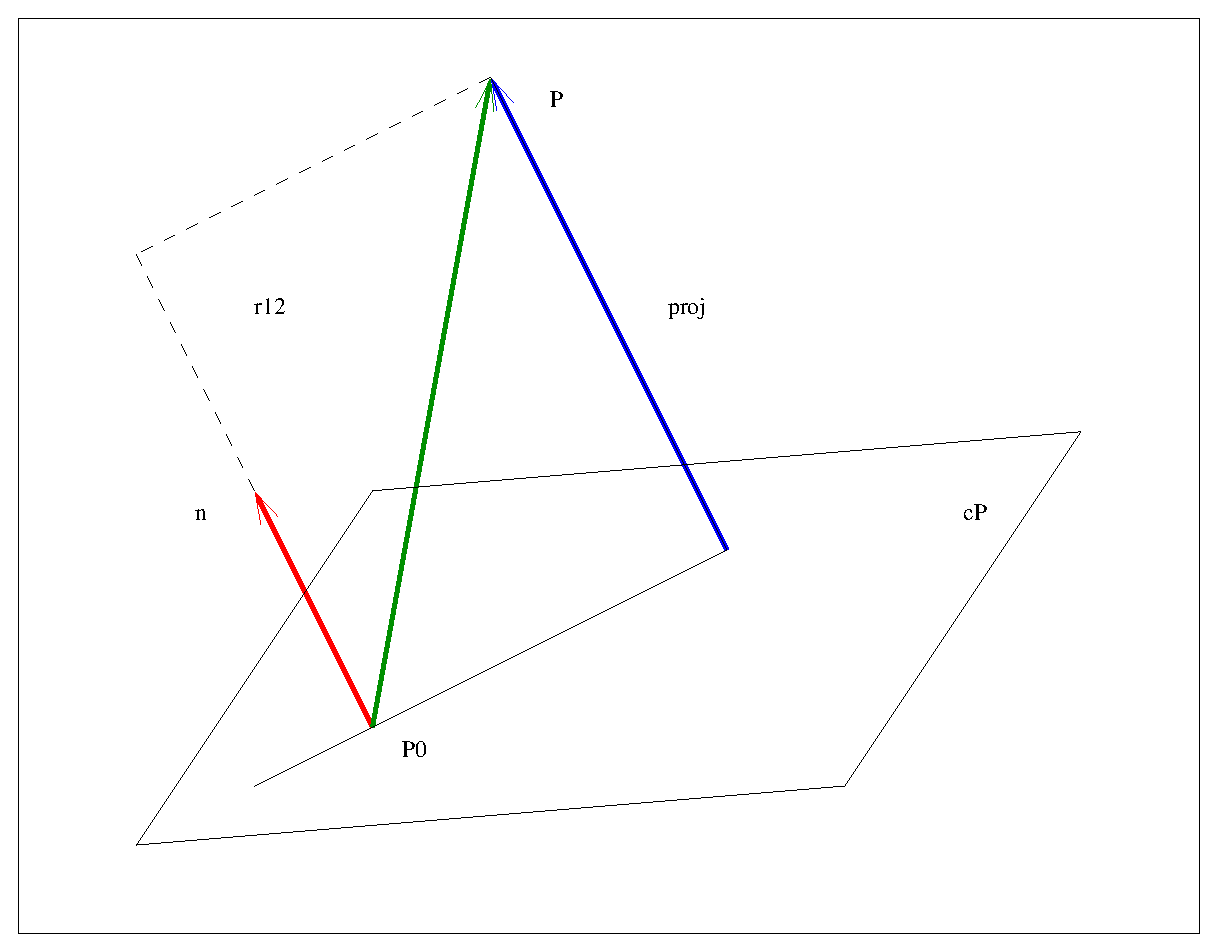
\includegraphics[height=2in]{../../modules/vectors/pictures/ok-distance_point_plane.eps}
    \end{figure}
    \end{columns}
\end{frame}
\begin{frame}
  \frametitle{Parallel lines}
    Lines
    $$L_1: \quad \textbf{r}= \textbf{r}_1+t\textbf{u}_1 \qquad L_2: \quad \textbf{r}= \textbf{r}_2+s\textbf{u}_2$$
\begin{columns}[t]
  \column[T]{6cm}
  \textcolor[rgb]{0.98,0.00,0.00}{Parallel} lines\\
    %\medskip
    \uncover<2->{
    $L_1 || L_2$ $\Longleftrightarrow$
    $\textbf{u}_1$, $\textbf{u}_2$ collinear $\Longleftrightarrow$
    $$\boxed{\textbf{u}_1 \times \textbf{u}_2 = \textbf{0}}$$}
    \uncover<3->{
    \textcolor[rgb]{0.98,0.00,0.00}{Distance}:
    $$d= d(L_1,L_2)  = d(P_1,L_2) = d(P_2,L_1)$$}
    \uncover<4->{
    $$d= d(L_1,L_2) = |\textbf{\text{orth}}_{\bm{u}_1} (\textbf{r}_2-\textbf{r}_1)|$$
    $$\boxed{d = \frac{|(\textbf{r}_2-\textbf{r}_1) \times \textbf{u}_1|}{|\textbf{u}_1|} =\frac{|(\textbf{r}_2-\textbf{r}_1) \times \textbf{u}_2|}{|\textbf{u}_2|}}$$}
    %\textcolor[rgb]{0.98,0.00,0.00}{Identical} lines: $d(L_1,L_2)=0$
    %$$\textbf{u}_1\times \textbf{u}_2 = \textbf{0} \text{ and }
    %(\textbf{r}_2-\textbf{r}_1) \times \textbf{u}_1 = \textbf{0}$$
  \column{6.5cm}
  \begin{figure}
        \psfrag{L1}{$L_1$}
        \psfrag{L2}{$L_2$}
        \psfrag{P1}{$P_1$}
        \psfrag{P2}{$P_2$}
        \psfrag{r21}{$\textbf{r}_2-\textbf{r}_1$}
        \psfrag{u1}{$\textbf{u}_1$}
        \psfrag{u2}{$\textbf{u}_2$}
        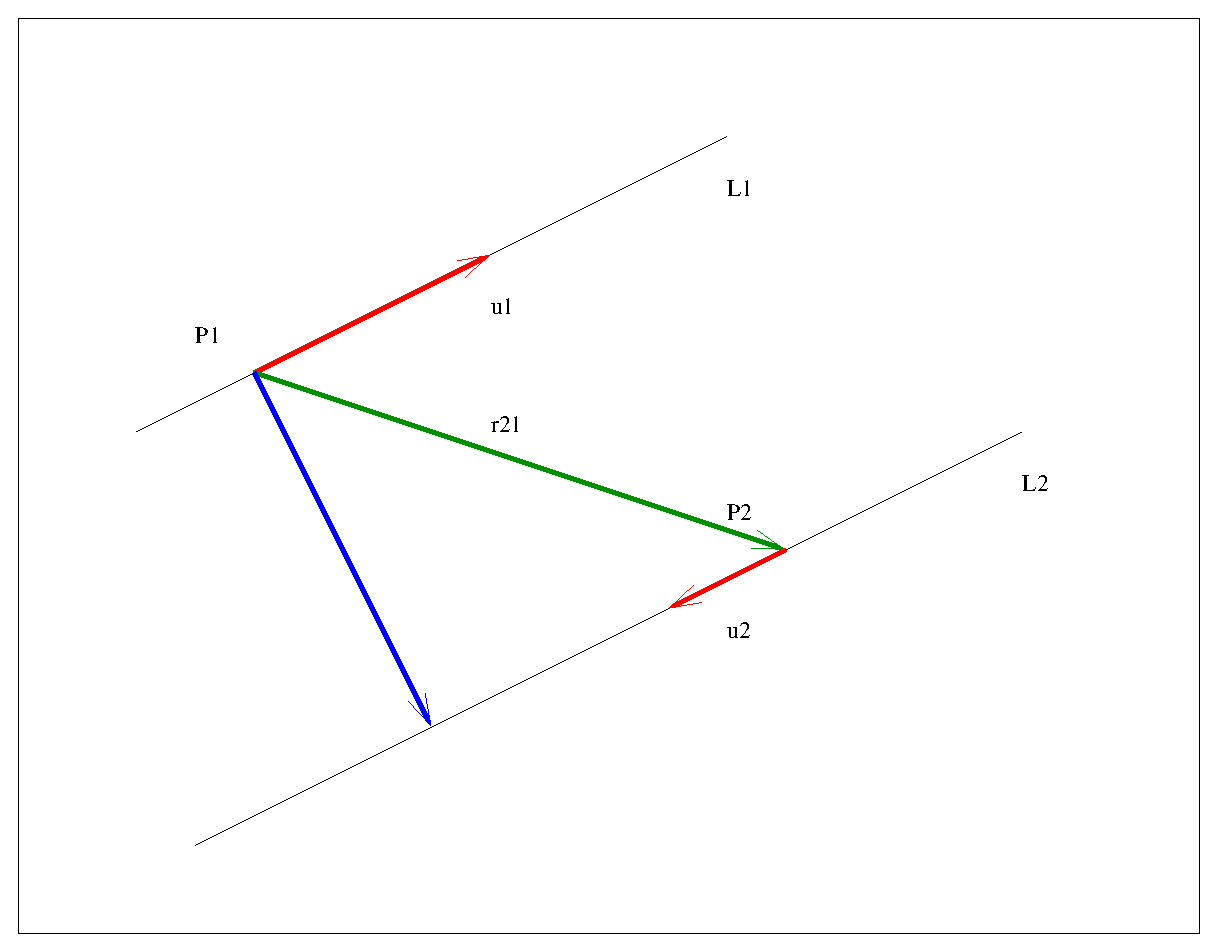
\includegraphics[height=2in]{../../modules/vectors/pictures/ok-distance_parallel_lines.eps}
    \end{figure}
\end{columns}

\end{frame}
\begin{frame}
\frametitle{Angle between lines}

\begin{columns}
\column{0.4\textwidth}
\begin{pspicture}(-2, -2)(2,2)
\tiny
\renewcommand{\fcScreen}{[-1 0 -0.5] 0}
\fcParallelogramIIId{[1.2 -1.2 1]}{[1.2 1.2 1]}{[-1.2 -1.2 1]}
\fcLineIIId{[-1 -1 -1]}{[1 1 -1]}
\fcPutIIId[l]{[1 1 -1]}{$L_2$}
\fcLineIIId{[1 -1 1]}{[-1 1 1]} 
\fcPutIIId[l]{[-1 1 1]}{$L_2$}
%\fcPerpendicularIIId[arrows=->, linecolor=green]{[0 0 -1]}{[1 -1 1] [-1 1 1]}{0.2}
\fcLineIIId[arrows=->, linecolor=blue]{[0 0 -1]}{[0 0 1]}
\fcLineIIId[linestyle=dotted]{[-1 -1 1]}{[1 1 1]}
\fcLineIIId[linecolor=red, arrows=->]{[0 0 -1]}{[0.75 0.75 -1]}
\fcPutIIId[t]{[0.325 0.325 -1.1]}{$\fcv u_1$}
\fcDotIIId{[0 0 -1]}
\fcPutIIId[r]{[-0.1 0.1 -1]}{$P_1~~~~$}


\fcDotIIId{[0 0 1]}
\fcPutIIId[r]{[-0.1 0.1 1]}{$P_2~~~~$}

\fcLineIIId[linecolor=red, arrows=->]{[0 0 1]}{[-0.75 0.75 1]}
\fcPutIIId[br]{[-0.325 0.325 1]}{$\fcv u_2$}

\fcLineIIId[linecolor=red, arrows=->]{[0 0 1]}{[0.75 0.75 1]}
\fcPutIIId[t]{[0.325 0.325 0.9]}{$\fcv u_1$}
\fcPutIIId[linecolor=brown]{[0 0 1]}{\fcAngleIIId{[0.5 0.5 0]}{[-0.5 0.5 0]}{0.2}}

\fcPutIIId{[2 2 0]}{%
\fcLineIIId[linecolor=red, arrows=->]{[0 0 1]}{[-0.75 0.75 1]}
\fcPutIIId[br]{[-0.325 0.325 1]}{$\fcv u_2$}
\fcLineIIId[linecolor=red, arrows=->]{[0 0 1]}{[0.75 0.75 1]}
\fcPutIIId[t]{[0.325 0.325 0.9]}{$\fcv u_1$}
\fcPutIIId[linecolor=brown]{[0 0 1]}{
\fcAngleIIId{[0.5 0.5 0]}{[-0.5 0.5 0]}{0.3}
\fcPutIIId[l]{[0 0.35 0]}{$\alpha$}
}
}%
\end{pspicture}
\column{0.6\textwidth}
\begin{itemize}
\item Given: lines $ \begin{array}{rrcl}L_1:&  \textbf{r}&=& \textbf{r}_1+t\textbf{u}_1 \\ L_2:& \textbf{r}&=& \textbf{r}_2+s\textbf{u}_2\end{array}$.
\item Goal: find angle between $L_1$ and $L_2$.
\end{itemize}
\alert<1->{Perpendicular} lines
\uncover<2->{
$L_1 \bot L_2$ $\Longleftrightarrow$
$\textbf{u}_1 \bot \textbf{u}_2$ $\Longleftrightarrow$
$$\boxed{\textbf{u}_1 \cdot \textbf{u}_2 = 0}$$}
\uncover<3->{
\alert<1->{Angle} between lines}
\uncover<4->{
$\alpha$: angle between $L_1$, $L_2$ $\Longleftrightarrow$ 
$\alpha$: acute angle $\textbf{u}_1$, $\textbf{u}_2$}
\uncover<5->{$\Longleftrightarrow$
$$\boxed{\alpha = \arccos\left( \frac{|\textbf{u}_1 \cdot \textbf{u}_2|}{|\textbf{u}_1| \, |\textbf{u}_2|}\right) }$$}
\end{columns}
\end{frame}
\begin{frame}
  \frametitle{Distance between lines}
     Lines
    $$L_1: \quad \textbf{r}= \textbf{r}_1+t\textbf{u}_1 \qquad L_2: \quad \textbf{r}= \textbf{r}_2+s\textbf{u}_2$$

   \begin{columns}[t]
    \column[T]{6cm}
    \textcolor[rgb]{0.98,0.00,0.00}{Skew lines}
    $$\textbf{n} = \textbf{u}_1 \times \textbf{u}_2 \neq \textbf{0}$$
    \textcolor[rgb]{0.98,0.00,0.00}{Distance}:
    $$
      d(L_1,L_2)  = |\textbf{\text{proj}}_{\bm{n}} (\textbf{r}_2-\textbf{r}_1)| =$$
      $$= \boxed{\frac{|(\textbf{r}_2-\textbf{r}_1)\cdot \textbf{n}|}{|\textbf{n}|}}=
      \frac{|(\textbf{r}_2-\textbf{r}_1)\cdot (\textbf{u}_1\times \textbf{u}_2)|}{|\textbf{u}_1\times \textbf{u}_2|}$$
    \textcolor[rgb]{0.98,0.00,0.00}{Intersecting} lines: $d(L_1,L_2)=0$
    $$\textbf{u}_1\times \textbf{u}_2 \neq \textbf{0}$$
    $$(\textbf{r}_2-\textbf{r}_1) \cdot (\textbf{u}_1\times \textbf{u}_2) = 0$$

    \column{6.5cm}
    \only<1>{\begin{figure}
        \psfrag{L1}{$L_1$}
        \psfrag{L2}{$L_2$}
        \psfrag{P1}{$P_1$}
        \psfrag{P2}{$P_2$}
        \psfrag{n}{$\textbf{n}$}
        \psfrag{r21}{$\textbf{r}_2-\textbf{r}_1$}
        \psfrag{u1}{$\textbf{u}_1$}
        \psfrag{u2}{$\textbf{u}_2$}
        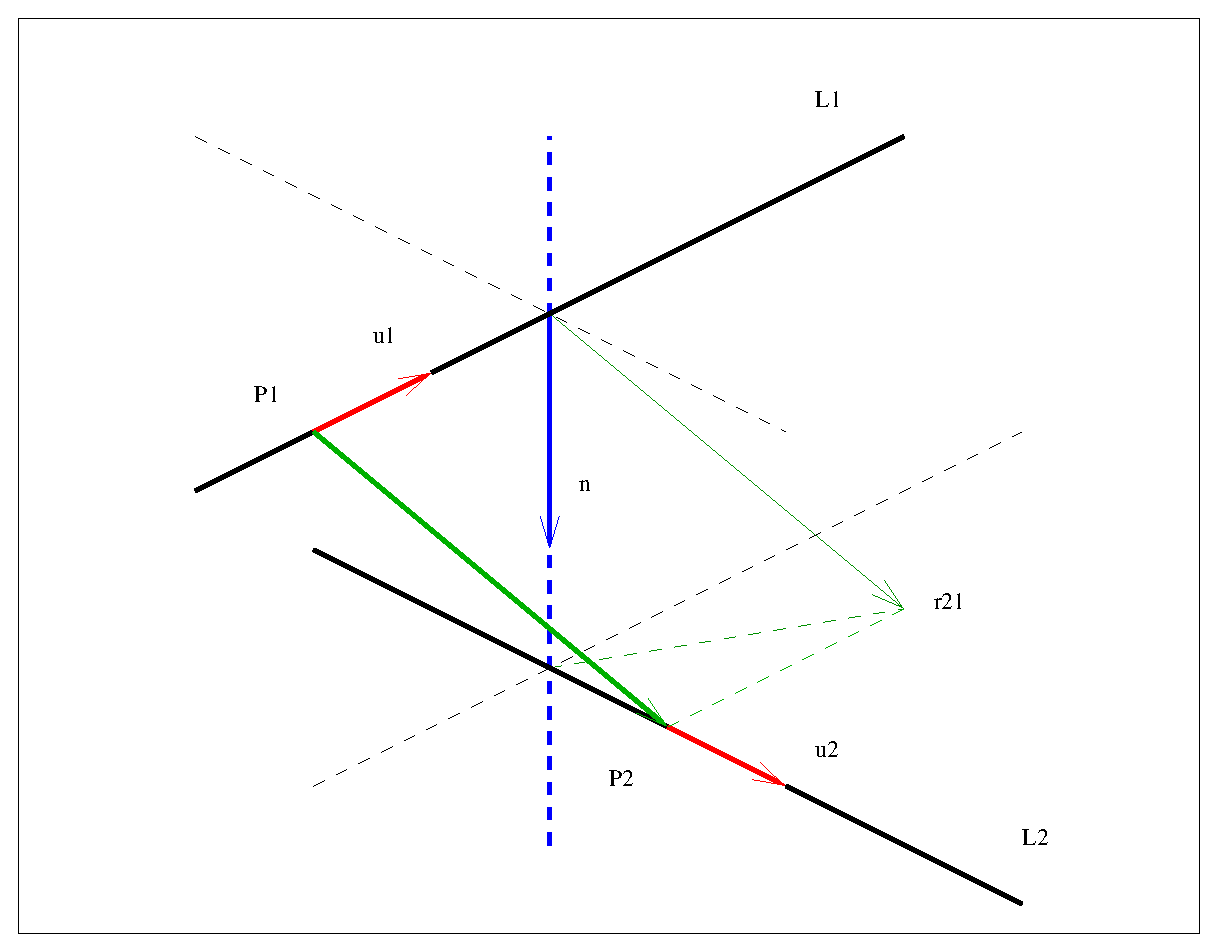
\includegraphics[height=2in]{../../modules/vectors/pictures/ok-distance_skew_lines.eps}
    \end{figure}}
    \only<2>{\begin{figure}
        \psfrag{L1}{$L_1$}
        \psfrag{L2}{$L_2$}
        \psfrag{P1}{$P_1$}
        \psfrag{P2}{$P_2$}
        \psfrag{n}{$\textbf{n}$}
        \psfrag{r21}{$\textbf{r}_2\!-\!\textbf{r}_1$}
        \psfrag{u1}{$\textbf{u}_1$}
        \psfrag{u2}{$\textbf{u}_2$}
        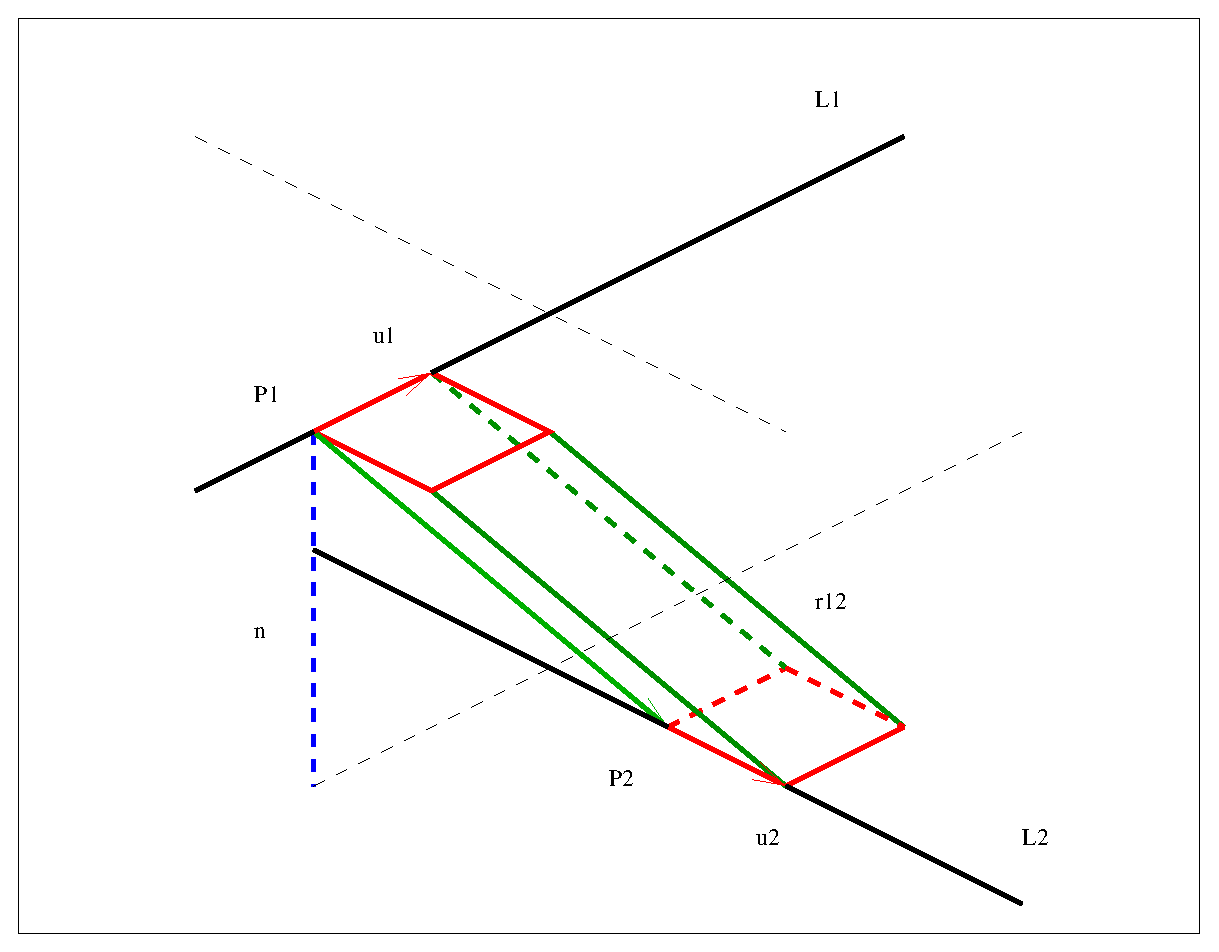
\includegraphics[height=2in]{../../modules/vectors/pictures/ok-distance_skew_lines_box.eps}
    \end{figure}
    }
  \end{columns}
\end{frame}

\begin{frame}
\frametitle{Distance between parallel line and plane}
\begin{columns}
\column{0.4\textwidth}
        \psfrag{L}{$L$}
        \psfrag{cP}{$\mathcal{P}$}
        \psfrag{P1}{$P_1(\fcv{r}_1)$}
        \psfrag{P0}{$P_0(\fcv{r}_0)$}
        \psfrag{u}{$\fcv{u}$}
        \psfrag{n}{$\fcv{n}$}
        \psfrag{r01}{$\fcv{r}_1-\fcv{r}_0$}
        \psfrag{proj}{$\fcv{\text{proj}}_{\bm{n}} (\fcv{r}_1\!-\!\fcv{r}_0)$}
        \psfrag{orth}{$\fcv{\text{orth}}_{\bm{u}}(\fcv{r}_1\!-\!\fcv{r}_0)$}
        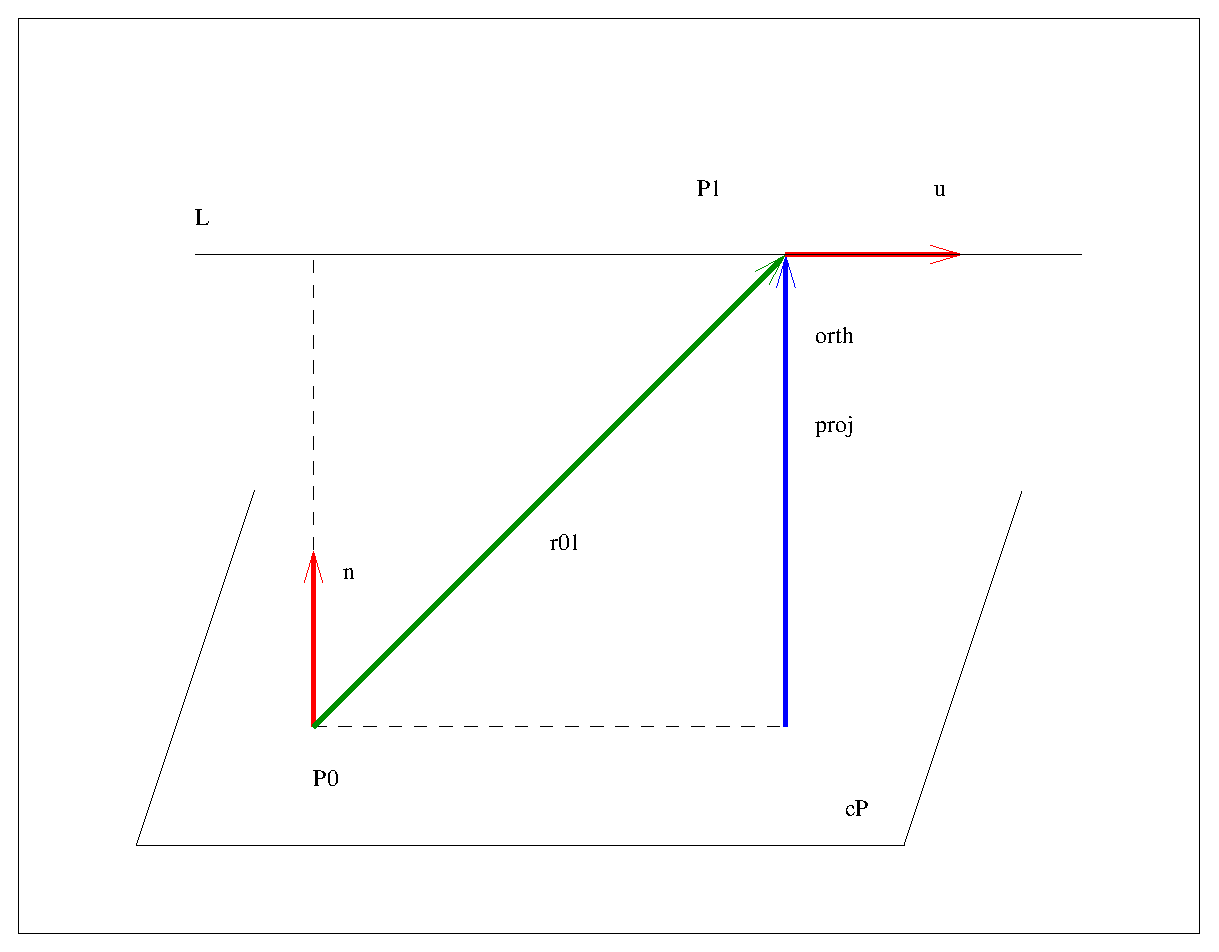
\includegraphics[height=1.4in]{../../modules/vectors/pictures/ok-parallel_line_plane.eps}
    
\column{0.6\textwidth}
\begin{itemize}
\item Given: line $L: \quad \fcv{r}= \fcv{r}_1+t\fcv{u}$,
\item plane $\mathcal{P}: \quad (\fcv{r}-\fcv{r}_0) \cdot \fcv{n} = 0$.
\item Goal: find distance between the the two.
\end{itemize}

\end{columns}
Line \alert<1->{parallel} to plane. \uncover<2->{
$L || \mathcal{P}$ $\Longleftrightarrow$
$\fcv{u} \bot \fcv{n}$ $\Longleftrightarrow$
$$\boxed{\fcv{u} \cdot \fcv{n} = 0}$$}
\uncover<3->{
\alert<1->{Distance} from $L$ to $\mathcal{P}$:
$d(L,\mathcal{P}) = d(P_1,\mathcal{P})$}
\uncover<4->{
$$d=|\fcv{\text{orth}}_{\bm{u}}(\fcv{r}_1-\fcv{r}_0)| =
\fcv{\text{proj}}_{\bm{n}} (\fcv{r}_1-\fcv{r}_0)|$$
$$d = \frac{|(\fcv{r}_1-\fcv{r}_0) \times \fcv{u}|}{|\fcv{u}|} =
\textcolor[rgb]{0.98,0.00,0.00}{\frac{|(\fcv{r}_1-\fcv{r}_0)\cdot \fcv{n}|}{|\fcv{n}|}}$$}
\end{frame}

\begin{frame}
\frametitle{Angle between line and plane}
\begin{columns}
\column{0.4\textwidth}
\psset{xunit=2cm, yunit=2cm}
\begin{pspicture}(-1.2, -1.2)(2,2)
\renewcommand{\fcScreen}{[-4 -1 -1] 0}
\tiny 
\fcParallelogramIIId{[-1 -1 0]}{[1 -1 0]}{[-1 1 0]}
\fcPutIIId{[-1 1 0]}{$\mathcal P$}
\fcPerpendicularIIId[linestyle=dotted]{[0.5 -0.7 0 ]}{[0 0.5 0] [0 0.5 1]}{0.2}
%\fcDotIIId{[0 0.5 1]}
%\fcPutIIId[b]{[0 0.5 1]}{$P_1(\fcv r_1)$}

\fcLineIIId[arrows=->, linecolor=blue]{[0 0.5 0]}{[0 0.5 1]}
\fcPutIIId[l]{[0 0.5 0.5]}{$\fcv{proj}_{\fcv n}(\fcv u)$}

\fcLineIIId[arrows=->, linecolor=red]{[0.5 -0.7 0]}{[0.5 -0.7 0.5]}
\fcPutIIId[r]{[0.5 -0.7 0.25]}{$\fcv n~~$}

\fcPerpendicularIIId[arrows=<-, linecolor=red]{[0.9 0.9 0.5]}{[0.9 0.9 0] [0.9 0.8 0]}{0.1}
\fcPutIIId[l]{[0.9 0.9 0.25]}{$~~\fcv n$}
\fcDotIIId{[0.9 0.9 0]}
\fcPutIIId[t]{[0.9 0.9 -0.1]}{$P_0(\fcv r_0)$}

\fcPutIIId{[0.5 -0.7 0]}{\fcAngleIIId {[-0.5 1.2 0]} {[-0.5 1.2 1]}{0.2}}
\fcPutIIId[l]{[0.4 -0.5 0.1]}{$\alpha$}

\fcLineIIId[arrows=->, linecolor=green]{[0.5 -0.7 0]}{[0 0.5 1]}
\fcLineIIId[linestyle=dotted]{[0.56 -0.844 -0.12]}{[0.5 -0.7 0]}
\fcLineIIId{[0.65 -1.06 -0.3]}{[0.56 -0.844 -0.12]}
\fcLineIIId{[0 0.5 1]}{[-0.15 0.86 1.3]}
\fcPutIIId[tl]{[0.65 -1.06 -0.3]}{$~~L$}

\fcPutIIId[tl]{[0.25 -0.1 0.5]}{$\fcv u$}

\fcLineIIId[linestyle=dotted]{[0.5 -0.7 0]}{[0.5 -0.7 0.9]}

\end{pspicture}
\column{0.6\textwidth}
\begin{itemize}
\item Given: line $L: \quad \fcv{r}= \fcv{r}_1+t\fcv{u}$,
\item plane $\mathcal{P}: \quad (\fcv{r}-\fcv{r}_0) \cdot \fcv{n} = 0$.
\item Goal: Find angle between line and plane.
\end{itemize}
\end{columns}
Line \alert<1->{perpendicular} to plane
\uncover<2->{
$L \bot \mathcal{P}$ $\Longleftrightarrow$
$\fcv{u} \| \fcv{n}$ $\Longleftrightarrow$ 
$\boxed{\fcv{u} \times \fcv{n} = \fcv{0}}$
}

\uncover<3->{
\alert<1->{Angle} between line and plane $\alpha$: angle between $L$, $\mathcal{P}$.
}
$\begin{array}{rcl}
%\sin \alpha &=& \frac{|\fcv{proj}_{\fcv n}\fcv u|}{|\fcv u|} = \frac{|u\cdot n| }{||}\\
 \alpha &=& \arcsin\left( \frac{|\fcv{u} \cdot \fcv{n}|}{|\fcv{u}| \, |\fcv{n}|}\right) 
\end{array}
$


\uncover<5->{\alert<1>{Intersection}:}

\uncover<6->{
$\begin{array}{rcl}
(\fcv{r}_1+t\fcv{u}-\fcv{r}_0) \cdot \fcv{n} &=& 0\\
(\fcv{r}_1-\fcv{r}_0)\cdot \fcv{n} + t \fcv{u} \cdot \fcv{n} &=& 0
\end{array}
$

Solve for $t$.
}
\end{frame}
\begin{frame}
  \frametitle{Parallel planes}
     Planes
     $\mathcal{P}_1: \quad (\textbf{r} - \textbf{r}_1) \cdot \textbf{n}_1 = 0$
     \hspace{2cm}
     $\mathcal{P}_2: \quad (\textbf{r} - \textbf{r}_2) \cdot \textbf{n}_2 = 0$

  \begin{columns}[t]
    \column[T]{6cm}
    \textcolor[rgb]{0.98,0.00,0.00}{Parallel} planes:  \\
    \uncover<2->{$\mathcal{P}_1 || \mathcal{P}_2$ $\Longleftrightarrow$ $\textbf{n}_1$, $\textbf{n}_2$ collinear $\Longleftrightarrow$
    $$\boxed{\textbf{n}_1 \times \textbf{n}_2 = \textbf{0}}$$}
    \uncover<3->{
    \textcolor[rgb]{0.98,0.00,0.00}{Distance} between parallel planes:
    $$d(\mathcal{P}_1,\mathcal{P}_2) =
    |\textbf{\text{proj}}_{\textbf{n}_1} (\textbf{r}_2-\textbf{r}_1)| = $$
    $$=\boxed{\frac{|(\textbf{r}_2-\textbf{r}_1)\cdot \textbf{n}_1|}{|\textbf{n}_1|}}$$}
    \uncover<4->{\textcolor[rgb]{0.98,0.00,0.00}{Scalar} equations:\\
    $\mathcal{P}_1 : \quad ax+by+cz = d_1$\\
    $\mathcal{P}_2 : \quad ax+by+cz = d_2$
    $$\boxed{d(\mathcal{P}_1,\mathcal{P}_2) = \frac{|d_2-d_1|}{\sqrt{a^2+b^2+c^2}}}$$}
    \column[T]{6.5cm}
    \begin{figure}
        \psfrag{cP1}{$\mathcal{P}_1$}
        \psfrag{cP2}{$\mathcal{P}_2$}
        \psfrag{P1}{$P_1(\textbf{r}_1)$}
        \psfrag{P2}{$P_2(\textbf{r}_2)$}
        \psfrag{n1}{$\textbf{n}_1$}
        \psfrag{n2}{$\textbf{n}_2$}
        \psfrag{r12}{$\textbf{r}_2\!-\!\textbf{r}_1$}
        \psfrag{proj}{$\textbf{\text{proj}}_{\bm{n}_1} (\textbf{r}_1\!-\!\textbf{r}_0)$}
        \includegraphics[height=2in]{../../modules/vectors/pictures/ok-parallel_plane_plane.eps}
    \end{figure}
    %
  \end{columns}
\end{frame}
\begin{frame}
\frametitle{Angle between planes}
\begin{columns}
\column{0.4\textwidth}
\psset{xunit=1.4cm, yunit=1.4cm}
\begin{pspicture}(-2, -2)(2,2)
\tiny
\renewcommand{\fcScreenStyle}{x}
%\fcAxesIIId{2}{2}{2}
\fcPolyLineIIId[linestyle=dashed]{[-1 -0.6 0] [-1 1 0] [0 1 0]}
\fcPolyLineIIId{[-1 -0.6 0] [-1 -1 0] [1 -1 0] [1 1 0] [0 1 0]}
\fcPolyLineIIId{[0 1 0] [-1 1 1] [-1 -1 1] [1 -1 -1] [1 1 -1] [0.33 1 -0.33]}%
\fcLineIIId[linestyle=dashed]{[0.33 1 -0.33]}{[0 1 0]}%
\uncover<4->{%
\fcPerpendicularIIId[arrows=<-, linecolor=red]{[1.7 0 0.3]}{[1 0 -1]}{0.2}%
\fcDotIIId{[0.7 0 -0.7]}%
\fcPutIIId[tl]{[0.7 0 -0.7]}{$~~P_1$}%
\fcPutIIId[l]{[1.5 0 0]}{$~\fcv n_1$}
}%
%\fcPerpendicularIIId[arrows=<-, linecolor=red]{[1 0 1]}{[-1 0 1]}{0.2}
\fcLineIIId[arrows=<-, linecolor=red]{[1 0 1]}{[0 0 0]}
\fcPutIIId[tl]{[0.85 0 0.85]}{$~~\fcv n_1$}%

\uncover<4->{%
\fcPerpendicularIIId[arrows=<-, linecolor=red]{[0.8 0.8 0.8]}{[0.8 0.8 0] [0.6 0.8 0]}{0.2}%
\fcDotIIId{[0.8 0.8 0]}
\fcPutIIId[bl]{[0.8 0.8 0]}{$~~P_2$}
\fcPutIIId[bl]{[0.8 0.8 0.5]}{$~~\fcv n_2$}
}%

\fcLineIIId[linecolor=gray]{[0 -1 0]}{[0 1 0]}

%\fcPerpendicularIIId[arrows=<-, linecolor=red]{[0 0 0.8]}{[-1 0 0]}{0.1}
\fcLineIIId[arrows=<-, linecolor=red]{[0 0 0.8]}{[0 0 0]}
\fcPutIIId[bl]{[0 0 0.5]}{$~~\fcv n_2$}

\fcPolyLineIIId{[-0.5 0 0.5] [0 0 0]}%
\fcLineIIId[linestyle=dashed]{[0 0 0]}{[0.2 0 -0.2]}%
\uncover<2-3>{%
\fcPerpendicularIIId{[-0.5 0 0.5]}{[0 1 0]}{0.2}%
}%
\fcLineIIId[linestyle=dashed]{[0 0 0]}{[-0.7 0 0]}%
\fcLineIIId{[0 0 0]}{[0.7 0 0]}%
\uncover<3>{%
\fcPerpendicularIIId[linestyle=dashed]{[-0.7 0 0]}{[0 1 0]}{0.2}%
}%
\uncover<4->{%
\fcAngleIIId[linecolor=blue]{[-1 0 1]}{[-1 0 0]}{0.3}%
\fcPutIIId[rb]{[-0.3 0 0.1]}{$\alpha$}%
}%

\fcAngleIIId[linecolor=blue]{[0 0 1]}{[1 0 1]}{0.3}

\fcLineIIId[arrows=->, linecolor=blue]{[0 0 0]}{[0 -0.8 0]}
\fcPutIIId[l]{[0 -0.5 0]}{$~\fcv u$}
\fcPutIIId[tr]{[-1 -1 0]}{$\mathcal P_2$}
\fcPutIIId[tr]{[-1 -1 1]}{$\mathcal P_1$}
%\fcParallelogramHollowIIId{[-1 -1 0]}{[1 -1 0]}{[-1 1 0]}
%\fcParallelogramHollowIIId{[1 -1 -1]}{[1 1 -1]}{[-1 -1 1]}
\end{pspicture}

\begin{pspicture}(-0.2, -0.2)(0.2, 0.2)
\renewcommand{\fcScreen}{[0 1 0] 0}
\fcLineIIId[arrows=<-, linecolor=red]{[0 0 0.8]}{[0 0 0]}
\fcPutIIId[bl]{[0 0 0.5]}{$~~\fcv n_2$}
\fcLineIIId[arrows=<-, linecolor=red]{[1 0 1]}{[0 0 0]}
\fcPutIIId[tl]{[0.85 0 0.85]}{$~~\fcv n_1$}%

\end{pspicture}

\column{0.6\textwidth}
\begin{itemize}
\item Given: planes 
$\begin{array}{rrcl}
\mathcal{P}_1:&  (\fcv{r} - \fcv{r}_1) \cdot \alert<4>{\fcv{n}_1 }&=& 0 \\
\mathcal{P}_2:& (\fcv{r} - \fcv{r}_2) \cdot \alert<4>{\fcv{n}_2} &=& 0
\end{array}
$
\item Goal: \alert<4>{define} and find the angle between the two planes.
\end{itemize}
\end{columns}
\begin{itemize}
\item<2-> In $\mathcal P_1$, drop perpendicular from point to intersection line.
\item<3-> In $\mathcal P_2$, raise a perpendicular from the perpendicular heel.
\item<4-> \alert<4>{Define angle $\alpha$} b-n $\mathcal P_1, \mathcal P_2$ = acute angle b-n two perpendiculars.
\end{itemize}


\alert<1->{Angle} $\alpha$ between planes:
\uncover<2->{
$
\begin{array}{rcl}
\alpha &=& \text{acute angle} (\fcv{n}_1,\fcv{n}_2) \\
\alpha &=&\arccos{\left( \frac{|\fcv{n}_1 \cdot \fcv{n}_2|}{|\fcv{n}_1|\, |\fcv{n}_2|}\right)}
\end{array}
$
}

\uncover<3->{\alert<1->{Perpendicular} planes:} \uncover<4->{$$\alpha = \frac{\pi}{2} \Longleftrightarrow \boxed{\fcv{n}_1 \cdot \fcv{n}_2 = 0}$$}
\uncover<5->{Direction of \textcolor[rgb]{0.98,0.00,0.00}{line of intersection}:}
\uncover<6->{$$\fcv{u} = \fcv{n}_1 \times \fcv{n}_2$$}
\end{frame}
} %end lecture

% begin lecture
\lect{2014}{Lecture 5}{5}{
\section{Functions of Several Variables}
%\begin{frame}
\begin{itemize}
\item So far, the functions we studied had  one dimensional (scalar) input.
\item<2-> Most mathematical models deal with phenomena where the output
depends on several variables.
\item<3-> Variables may be ``dependent'' or independent - issue dealt with in the subject of probabilities/statistics.
\item<4-> We need to build and use functions with multidimensional input.
\item<5-> Such input is typically represented as a bundle of scalar variables.
\end{itemize}

\end{frame}
\subsection{Verbal description}
%\begin{frame}\frametitle{Describing multivariable functions}
\begin{itemize}
\item Several ways to define a function of several variables. 
\item Usually: start with \emph{verbal} description, then give specific meanings
to our input and output variables. 
\item We explain by examples.
\end{itemize}
\end{frame}

\begin{frame}\frametitle{Verbal description examples}
\begin{itemize}
  \item The apparent temperature, $W$, felt on exposed skin
  depends on several factors, including the actual
  temperature, $T$, the wind speed, $v$, and the humidity.
  The \emph{wind chill temperature} is a mathematical model
  for $W$ under the assumption that the humidity is 0 and
  that the only factors influencing $W$ are $T$ and $v$:
  %
  $$W = W(T,v)\; .$$
  %
  The domain of the function $W$ consists of all reasonable
  pairs $(T,v)$.

  \item The Cobb-Douglas production function models the
  production output, $P$, under the assumption that the
  only factors are the amount of labor, $L$, and the
  amount of capital, $K$:
  %
  $$P=P(L,K) \; .$$
\end{itemize}

\vskip 8cm %to serve for spacing
\end{frame}
\begin{frame}\frametitle{Verbal description examples}
\begin{itemize}
%  \item The magnitude $G$ of the attraction force between
%  two bodies depends on several factors, including the
%  masses $m$ and $M$ of the bodies and the distance $d$
%  between them:
  %
%  $$G=G(m,M,d)$$

  \item A set $(\rho, \phi, \theta)$ of spherical
  coordinates determines the rectangular coordinates
  $(x,y,z)$ of a point. In this case, both the input
  and the output are multidimensional:
  %
  $$(x,y,z) = \textbf{F}(\rho, \theta, \phi)\; ,$$
  %

  \item The wind velocity $\textbf{v}$ at a point $P$
  depends on the position $\textbf{r}$ of $P$,
  %
  $$\textbf{v} = \textbf{V} (\textbf{r})\; .$$
  %
  In this case both the input and the output are
  vectorial quantities.

  \item The electric force on a charge $q$ displaced
  by $\textbf{r}$ from a charge $Q$ depends on the
  two charges, the displacement, and the medium in
  which the charges are placed:
  %
  $$\textbf{E} =
  \textbf{E}(q, Q,\textbf{r})\; .$$
  %
  Note that in this case the output data
  is a vector and the input data is a mix of scalar
  and vectorial quantities.
\end{itemize}

\vskip 8cm %to serve for spacing

\end{frame}
\subsection{Numerical description}
%\begin{frame}
\frametitle{Numerical description}
\begin{itemize}
\item Verbal description is essential for understanding.
\item<2-> However this does not include quantitative or visual information.
\item<3-> A \emph{numerical} description gives output data for a relevant set of input data.
\item<4-> This facilitates construction/study of a mathematical model.
\item<5-> Numerical description is typically given by table.
\item<6-> This table contains numerical data collected through experiments at selected input levels. 
\end{itemize}
\end{frame}

\begin{frame}
\frametitle{Examples: describing multivariable function via numerical data.}
\begin{itemize}
\item the following is Wind Chill Chart provided by NOOA:
\includegraphics[width=3in]{../../modules/multivariable-functions/pictures/windchill2.jpg}
\end{itemize}
\end{frame}
\begin{frame}
\begin{itemize}
\item Another example is the Income Tax Table. Explain what the
input and output variables are in that case.
\end{itemize}
\end{frame}
\subsection{Analytical description} 
%\begin{frame}\frametitle{Analytical description of multivarible function}

\begin{itemize}
\item Numerical data has output data for selected inputs only. 
\item<2-> If output is not tabulated for given input we need to approximate.
\item<3-> This is done by inter/extrapolation from given information. 
\item<4-> It would be better to have procedure to determine output from any reasonable input. 
\item<5-> This would be an \emph{analytical} description of the function. 
\item<5-> By analytical description we mean giving a procedure to compute the value of the function:
\begin{itemize}
\item<6-> via formula or
\item<7-> via another algorithmic procedure.
\end{itemize}

\end{itemize}
\end{frame}
\begin{frame}\frametitle{From numerical to analytical description}

\begin{itemize}
\item<1-> One way is to try to guess a formula that fits approximately the input data. 
\item<2-> For wind chill, one such formula is:
\[
W(T,v)= 35.74+0.6215 T - 35.75 v^{0.16} +0.4275 Tv^{0.16}
\]
with $W$ and $T$ in Fahrenheit and $v$ in $mph$.
\item<3-> A proper mathematical model requires that we
\begin{itemize}
\item<4-> compute unknown output for some input and 
\item<5-> make a new measurement and compare with the model's output to see if model gives correct prediction.
\end{itemize}
\item<6-> Constructing mathematical models to fit numerical data (approximately) is the subject of ``\alert<8>{Approximation theory}''. 
\item<7-> Mathematicians dealing with ``\alert<8>{approximation theory}'' are often called ``applied mathematicians''.
\item<8-> The \alert<8>{above terms} are not precisely defined and not fully agreed upon. 
\end{itemize}
\end{frame}
\begin{frame}
\begin{itemize}
\item For the Cobb-Douglas production function: economic analysis motivates properties such function should have. 
\item One formula (model) with these properties is:
\[
P(K,L) = cL^a K^{1-a}\; ;
\]
where $a$ is a parameter between $0$ and $1$. 
\item While the function $P$ depends on three variables $a$, $L$, and $K$, we treat them differently: we consider $a$ to be a parameter of the model; once we decide on the value of $a$, we treat it as a constant.
\item The transition formulas from spherical to rectangular coordinates are a derived via geometric reasoning.
\end{itemize}
\end{frame}

\begin{frame}
\begin{itemize}
\item An important class of functions of several variables is the class of polynomial functions. Polynomials of degree one are
\begin{align*}
f(x,y) = & ax+by+c \\
g(x,y,z) = & ax+by+cz+d  \; ,
\end{align*}
and polynomials of degree two are
\begin{align*}
f(x,y) = & \; a_{11}x^2+a_{12}xy+a_{22}y^2+ a_1 x + a_2 y + a_0 \\
g(x,y,z) = & \; a_{11} x^2 + a_{22}y^2 + a_{33}z^2 + a_{12}xy + a_{13}xz+a_{23}yz + \\
& + a_1 x + a_2 y + a_3 z + a_0
\end{align*}
where the $a_{ij}$'s are real numbers.
\end{itemize}
\end{frame}
\begin{frame}
\begin{itemize}
\item The formula for electric force is given by laws of physics: the magnitude of the force is directly proportional to the charges $q$, $Q$, and inversely proportional to the square of the distance between them. The force acts along the line joining the two points, attracts $q$ to $Q$ if the charges have different sign and rejects $q$ from $Q$ if the charges have the same sign. The mathematical translation is
\[
\textbf{E}(q, Q, \textbf{r}, \epsilon) = \frac{\epsilon q Q}{|\textbf{r}|^3} \textbf{r}\; ,
\]
where $\epsilon$ is a proportionality constant, depending on the medium the charges are placed in.
\end{itemize}
\end{frame}

\section{Graphical descriptions}
\subsection{Functions of two variables}
%\begin{frame}
\begin{itemize}
\item An analytical description is technically best, but not easy to interpret.
\item If output is a scalar, where does the function attain its extreme values (maxima, minima)?  
\item How do values change for nearby points - are they decreasing, increasing, how fast?
\item We will learn to decode this information from the analytical descriptions.
\item Even so, ``a picture is worth a thousand words (and, say, 10 f-las)''.
\end{itemize}
\end{frame}

\begin{frame}
\begin{center}
\psset{xunit=1cm,yunit=1cm}
\begin{pspicture}(-3,-3)(3,5.5)

\psset{Beta=15}
\psplotThreeD[plotstyle=line,drawStyle=xLines,yPlotpoints=50,xPlotpoints=50,linewidth=0.3pt, linecolor=blue](-4,4)(-4,4){ x 3 exp x y 4 exp mul add x 5 div sub 10 mul 2.729 x dup mul y dup mul add neg exp mul 2.729 x 1.225 sub dup mul y dup mul add neg exp add}
\pstThreeDCoor[xMin=-1,xMax=5,yMin=-1,yMax=5,zMin=-1,zMax=5]
\rput[t](-3,5.3){Graph of a scalar function.}
\end{pspicture}
\end{center}

\end{frame}

\begin{frame}\frametitle{Graph of a function}
\begin{itemize}
\item For one variable function, $y=f(x)$, the graph of $f$ is a set of points in $\RR^2$: the set of points $(x,y)$ such that $y=f(x)$.
\item Example: if $f(x) = x^2$, then  $(3,9)$ is on the graph, because $9=3^2$, but $(2,5)$ is not because $5 \neq 2^2$.
\item We can extend this graphical representation for functions with two dimensional input and one dimensional (scalar) output. 
\item The \emph{graph} of the function $f\colon D \to \RR$, where $D$ is a region in $\RR^2$, is the set of points $P(x,y,z)$ in $\RR^3$ whose coordinates satisfy the condition 
\[
z=f(x,y)\quad .
\]
\item For example, the graph of $f(x,y) = 2x-y+3$ is the set
\[
\{ (x,y,z) \, | \, z= 2x-y+3\} \Longrightarrow \text{ plane } 2x-y-z+3=0 \; .
\]

\end{itemize}

 



\end{frame}

\subsection{Slices and level curves}
%\begin{frame}
\frametitle{A motivating example}
What does the graph $\Gamma$ of $g$ look like?
\[
g(x,y) =x^2+2y^2\quad .
\]

\begin{pspicture}(-2,-2)(2,2)
\psC

\end{pspicture}

\begin{itemize}
\item The graph $\Gamma$ is the set of points $P(x,y,z)$ in $\RR^3$ such that $z=x^2+2y^2$. The set is not a plane: what does it look like?
\item To answer look at sections. Use imaginary CT scan to cut the graph; assemble resulting sections into a graph.
\item Cut by vertical planes parallel to the $Oyz-$plane.
\item Suppose cutting plane has equation $x=a$, where $a$-constant. Intersection with cutting plane is given by points:
\[
\{(a, y, z)\quad \text{where } z=a^2+2y^2)\}
\]
\item These cross-sections are parabolas lying inside the plane $x=a$ with vertices at $(a,0,a^2)$. The vertex rises as $a$ gets away from $0$.
\item When we intersect $\Gamma$ with the plane $x=a$ we treat $x$ as a constant and study the function $y\to z=g(a,y) = a^2+2y^2$.
\end{itemize}



Similarly, if we cut by planes $y=a$ we get partial
functions $x\to x^2+2a^2$, whose graphs are also
parabolas. Each such a parabola is now situated in the
vertical plane $y=a$. Hence vertical sections are
parabolas, with vertices rising as
we move farther away from the coordinate planes.

To get horizontal sections we have to
keep constant not an input variable, but the output
variable, $z$. Intersecting the graph of $g$ with
the plane $z=a$ we get a curve of equations $x^2+2y^2=a$,
$z=a$. For $a<0$ the intersection is empty, for $a=0$ it
consists of a single point, $(x,y,z) = (0,0,0)$, and for
$a>0$, the intersection is an ellipse in the plane $z=a$.

The \emph{level curve} corresponding to $z=a$ is the curve
$g(x,y)=a$ in the domain of $g$, with a label $a$ to
indicate the level of the output corresponding to
that level curve. Note that the level curve is not the
intersection of the graph of $g$ with the plane $z=a$;
instead, it is the projection of that intersection onto
the plane $Oxy$, where the domain of $g$ resides.

You should be familiarized with level curves if
you have ever seen a topographic map or if you
opened the newspaper at the weather section. What are the
functions in those cases?

\end{frame}


\subsection{Level sets}
The examples considered in the previous sections were all
examples of functions with scalar output and a two
dimensional input. Their graphs lived in
$\RR^3 = \RR^{2+1}$, with the 2 coming from the dimension
of the input and the 1 from the dimension of the output.
If we wanted to extend that graphic construction to
functions depending on three scalar variables,
we'd need $3+1=4$ dimensions for the graphs, and that
is momentarily impossible. The rescue comes from the
second graphical representation, using level sets,
because the level sets (with appropriate labeling of
the level) can be represented in a space with dimension
equal to the dimension of the input space.


For example, let $f(x,y,z) = ax+by-z$. The graph is the
quadruple $(x,y,z,w)$ in $\RR^4$ such that
$w = ax+by-z$, and we can't yet represent that
graphically. But the level set $f(x,y,z) = d$ is the
surface $ax+by-z = d$ in $\RR^3$, and that surface is a
plane. Level sets corresponding to equidistant values
$d_1$, $d_2$, and $d_3$ of the output are parallel
planes of equations
%
\begin{align*}
  \mathcal{P}_1 = f^{-1}(d_1) & \colon \; ax+by-z = d_1\\
  %
  \mathcal{P}_2 = f^{-1}(d_2) & \colon \; ax+by-z = d_2\\
  %
  \mathcal{P}_3 = f^{-1}(d_3) & \colon \; ax+by-z = d_3
\end{align*}
%
and these planes are also equidistant.

The following remark will play a very important role in
understanding surfaces in space.

\begin{remark}{\rm The level set $f(x,y,z)=0$ for the
function
%
$$f(x,y,z) = ax+by-z+d$$
%
is the same as the graph
of the function $g(x,y) = ax+by+c$.
}\end{remark}

We will see that while graph surfaces can always be
represented as level surfaces, the converse is not true:
level surfaces can't always be represented as graph
surfaces. However, we'll show that under some reasonable
assumptions, level surfaces can \emph{locally} be
described as graph surfaces. An illuminating example is
that of a sphere (centered at the origin): it is the
level surface of $f(x,y,z) = x^2+y^2+z^2$, but it can't
be globally represented as a graph surface. Try and see
what goes wrong!

\subsection{Level sets}
%\begin{frame}
\begin{itemize}
\item<1-> Previously we considered functions $\alert<2,6>{z}= g(\alert<3,5>{x,y})$  \alert<2>{with scalar output} and \alert<3>{two dimensional input}.
\item<4-> The graphs of such functions live in $\RR^3 = \RR^{\alert<5>{2} +\alert<6>{1}}$.
\item<5-> \alert<5>{2 dimensions} were used to represent the input.
\item<6-> \alert<6>{1 dimension} was used to represent the output.
\item<7-> To represent functions with 3 dimensional input (3 variables) and scalar output: need  $3+1=4$ dimensions.
\item<8-> That's difficult for eyes used to visualizing physical 3d- space.
\item<9-> Instead: label the level sets of the function with color or other means to indicate value.
\item<10-> In this way we represent the f-n graphically using dimension equal to the number of input variables.
\end{itemize}
\end{frame}
\begin{frame}
\frametitle{Example}
\begin{columns}
\column{0.4\textwidth}
\psset{xunit=0.4cm, yunit=0.4cm}
\begin{pspicture}(-4,-7)(6,10)
\renewcommand{\fcScreen}{[-1 1 -0.7] -1}
\fcBoundingBox{-4}{-8.5}{4}{10.5}
\tiny
\fcAxesIIIdFull{5}{5}{5}%
\uncover<5->{%
%d=4
\fcParallelogramIIId[linecolor=cyan!90]{[-2 -2 -8]}{[-2 3 -3]}{[5 -2 -1]}%
\fcPutIIId[l]{[2 2 0]}{$~~d=4$}%
\fcLineIIId{[0 0 0]}{[0 0 -4]}
\fcLineIIId{[0 0 0]}{[4 0 0]}
}%
\uncover<6->{%
%d=2
\fcParallelogramIIId[linecolor=cyan!70]{[-2 -2 -6]}{[-2 3 -1]}{[5 -2 1]}%
\fcPutIIId[l]{[2 2 2]}{$~~d=2$}%
\fcLineIIId{[0 0 0]}{[0 2 0]}
\fcLineIIId{[0 0 0]}{[2 0 0]}
\fcLineIIId{[0 0 0]}{[0 0 -2]}
}%
\uncover<7->{%
%d=0
\fcParallelogramIIId[linecolor=cyan!50]{[-2 -2 -4]}{[-2 3 1]}{[5 -2 3]}%
\fcPutIIId[l]{[2 2 4]}{$~~d=0$}%
\fcLineIIId{[0 0 0]}{[0 0 4]}
\fcLineIIId{[0 0 0]}{[-4 0 0]}
\fcLineIIId{[0 0 0]}{[0 -4 0]}
}%
\uncover<8->{%
%d=-2
\fcParallelogramIIId[linecolor=cyan!30]{[-2 -2 -2]}{[-2 3 3]}{[5 -2 5]}%
\fcPutIIId[l]{[2 2 6]}{$~~d=-2$}%
\fcLineIIId{[0 0 2]}{[0 0 4]}%
\fcLineIIId{[-2 0 0]}{[-4 0 0]}%
\fcLineIIId{[0 -2 0]}{[0 -5 0]}%
}%
\uncover<9->{%
%d=-4
\fcParallelogramIIId[linecolor=cyan!10]{[-2 -2 0]}{[-2 3 5]}{[5 -2 7]}%
\fcPutIIId[l]{[2 2 8]}{$~~d=-4$}
\fcPutIIId[l]{[2 2 6]}{$~~d=-2$}%
\fcLineIIId{[0 0 4]}{[0 0 5]}%
\fcLineIIId{[-4 0 0]}{[-5 0 0]}%
}%
\fcAxesIIIdFull[arrows=->, linestyle=dotted, dash=1pt]{5}{5}{5}
\end{pspicture}

\column{0.6\textwidth}
\begin{itemize}
\item<1-> Let $f(x,y,z) = x+y-z$.
\item<2-> The graph consists of the quadruples $(x,y,z,w)$ in $\RR^4$ such that $w = x+y-z$. Can't plot that graphically (yet).
\item<3-> However, can represent with labeled level sets.
\item<4-> The level set $f(x,y,z) = d$ is the surface $x+y-z = d$ in $\RR^3$, and that surface is a plane.
\item<5-> For varying values of $d$ we plot the level set. 
$f(x,y,z) = \only<5>{d=4}\only<6>{d=2} \only<7>{d=0}\only<8>{d=-2}
\only<9>{d=-4}$.

Darker color = larger $d$.
\end{itemize}
\end{columns}

\end{frame}

\begin{frame}
To understand surfaces in space we need the following.
\begin{remark} The level set $f(x,y,z)=0$ for the function
%
$$f(x,y,z) = ax+by-z+d$$
%
is the same as the graph of the function $g(x,y) = ax+by+c$.
\end{remark}
\begin{itemize}
\item<2-> Graph surfaces can always be represented as level surfaces
\item<3-> The converse is not true: level surfaces can't always be represented as graph surfaces. 
\item<4-> Example: a sphere centered at the origin is the
level surface of $f(x,y,z) = x^2+y^2+z^2$ but it ``fails the vertical line test in all directions'', so it cannot be globally represented as a graph surface, no matter how we change the coordinate system.
\item<5-> We'll show that under reasonable assumptions, level surfaces can \emph{locally} be described as graph surfaces. 
\end{itemize}
\end{frame}





\subsection{Vector Fields}
%\begin{frame}
\frametitle{Vector fields}
\begin{itemize}
\item \emph{Vector fields} are functions with multidimensional input and output. 
\item Input is point in space; output is a vector, which we plot as a vector with a tail at the input point. 
\item Examples
\begin{itemize}
  \item Velocity of fluid/air at given point;
  \item Electric force per unit of charge;
  \item Gravitational field;
  %\item Fundamental directions $\textbf{e}_\rho$, $\textbf{e}_\phi$, $\textbf{e}_\theta$, $\textbf{e}_r$
\end{itemize}
\end{itemize}
\end{frame}

\begin{frame}
\frametitle{Coordinate representation of vector fields}

\begin{itemize}
\item<1-> In rectangular coordinates a vector field $\textbf{F}$ can
be decomposed along the fundamental directions:
$$
\textbf{F}(x,y,z) = F_1(x,y,z) \textbf{i} + F_2(x,y,z) \textbf{j} + F_3(x,y,z) \textbf{k} \; .
$$
\item<2-> For regions in the plane 2-dim vector fields are defined in a similar fashion: as function from subsets of $\mathbb R^2$ to $\RR$:
$$
\textbf{F}(x,y) = F_1(x,y) \textbf{i} + F_2(x,y) \textbf{j}
$$


\end{itemize}
\end{frame}
\begin{frame}
\begin{itemize}
\item<1-> Example: define the vector field $\textbf{e}_r$ on $\mathbb{R}^2 \setminus \{ (0,0)\}$ via
$
\textbf{e}_r = \cos\theta\, \textbf{i} +
\sin\theta \,\textbf{j} = \frac{x}{r} \, \textbf{i} +
\frac{y}{r} \, \textbf{j} = \frac{x}{\sqrt{x^2+y^2}} \,
\textbf{i} + \frac{y}{\sqrt{x^2+y^2}} \, \textbf{j}
$

\item<2-> Similarly define the vector field $\textbf{e}_{\theta}$ by:
$\textbf{e}_\theta = -\sin\theta\, \textbf{i} +
\cos\theta \,\textbf{j} = -\frac{y}{r} \, \textbf{i} +
\frac{x}{r} \, \textbf{j} = -\frac{y}{\sqrt{x^2+y^2}} \,
\textbf{i} + \frac{x}{\sqrt{x^2+y^2}} \, \textbf{j} \; .
$
\uncover<3->{
\psset{xunit=0.3cm, yunit=0.3cm}
\begin{pspicture}(-5.2,-5.2)(5.2,5.2)
\tiny
\fcAxesStandard{-5.1}{-5.1}{5.1}{5.1}
\fcVectorField[linecolor=blue, arrows=->]{-5}{-5}{11}{11}{1} {1 dict begin /r x x mul y y mul add sqrt def  r 0 eq {0 0} {x r div  y r div} ifelse end}
\end{pspicture}
\psset{xunit=0.3cm, yunit=0.3cm}
~~~ \begin{pspicture}(-5.2,-5.2)(5.2,5.2)
\tiny
\fcAxesStandard{-5.1}{-5.1}{5.1}{5.1}
\fcVectorField[linecolor=blue, arrows=->]{-5}{-5}{11}{11 }{1}{1 dict begin /r x x mul y y mul add sqrt def  r 0 eq {0 0} {-1 y mul r div  x r div} ifelse end}
\end{pspicture}
}
\item<4-> From the picture it is evident what trajectory would be followed by an object that ``\alert<5>{flows along the vector field}''.
\item<5-> By ``\alert<5>{flowing}'' we mean an object whose \alert<5>{velocity} at each point is given by \alert<5>{the value of the field}.
\end{itemize}
\end{frame}





%%%%%%%%%%%%%%%%%%


%%%%%%%%%%%%%%%%%%%%%%%%

\section{Surfaces}

\subsection{Quadric Surfaces}

Level sets for second degree polynomial functions

$$f(x,y,z) = Ax^2+By^2+Cz^2+Dxy+Exz+Fyz+Gx+Hy+Iz+J$$

\begin{itemize}
  \item At least one of $A$, $B$, $C$, $D$, $E$, or $F$ is non-zero;
  \item Some coefficients may be zero.
\end{itemize}

Level set $f(x,y,z)=k$ is called a \emph{quadric surface}. It suffices to consider $k=0$.

Through rigid motions (translations and rotations) it can be reduced to one of the following canonical forms (for different values of $A$, $B$, and $C$):
%
$$
  Ax^2+By^2+Cz^2+D = 0 \quad \text{ or } \quad
  Ax^2+By^2+Iz=0
$$
%
with not all of $A$, $B$, and $C$ equal to zero and $I$ not zero.

\begin{equation*}
Ax^2+By^2+Cz^2+D = 0
\end{equation*}

\begin{table}
\begin{tabular}{|c|c|c|c|c|c|c|c|c|}
  \hline
  % after \\: \hline or \cline{col1-col2} \cline{col3-col4} ...
  A & B & C & D & $x=x_0$ & $y=y_0$ & $z=z_0$ & Example & Name
  \\
  \hline
  $>0$ & $>0$ & $>0$ & $>0$ & empty & empty & empty & $x^2+2y^2+3z^2+4=0$ & empty \\
  \hline
  $>0$ & $>0$ & $>0$ & $=0$ &  &  &  &  &  \\
  \hline
  $>0$ & $>0$ & $>0$ & $<0$ & ellipse & ellipse & ellipse & $x^2+2y^2+3z^2-4=0$ & Ellipsoid \\
  \hline
  $>0$ & $>0$ & $=0$ & $>0$ &  &  &  &  &  \\
  \hline
  $>0$ & $>0$ & $=0$ & $=0$ &  &  &  &  &  \\
  \hline
  $>0$ & $>0$ & $=0$ & $<0$ &  &  &  &  &  \\
  \hline
  $>0$ & $>0$ & $<0$ & $>0$ &  &  &  &  &  \\
  \hline
  $>0$ & $>0$ & $<0$ & $=0$ &  &  &  &  &  \\
  \hline
  $>0$ & $>0$ & $<0$ & $<0$ &  &  &  &  &  \\
  \hline
  $>0$ & $=0$ & $=0$ & $>0$ &  &  &  &  &  \\
  \hline
  $>0$ & $=0$ & $=0$ & $=0$ &  &  &  &  &  \\
  \hline
  $>0$ & $=0$ & $=0$ & $<0$ &  &  &  &  &  \\
  \hline
\end{tabular}
\caption{Quadrics with central symmetry}
\end{table}

Fill in the rest of the table.

\bigskip


\begin{equation*}
Ax^2+By^2+Iz=0
\end{equation*}

\begin{table}
\begin{tabular}{|c|c|c|c|c|c|c|}
  \hline
  % after \\: \hline or \cline{col1-col2} \cline{col3-col4} ...
  A & B  & $x=x_0$ & $y=y_0$ & $z=z_0$ & Example & Name
  \\
  \hline
  $>0$ & $>0$   & parabola & parabola & ellipse, point, or empty & $x^2+2y^2+3z=0$ & Elliptic paraboloid \\
  \hline
  $>0$ & $=0$ & &  &  &  &   \\
  \hline
  $>0$ & $<0$ &  &  &  &  &   \\
  \hline
\end{tabular}
  \caption{Quadrics without central symmetry}
\end{table}
\bigskip

Fill in the rest of the table.


\subsection{Implicit functions}

A surface $S$ can be given in two different ways:

\begin{itemize}
  \item Implicit form, as a \emph{level surface}:
  %
  $$F(x,y,z) = k$$
  %
  \item  Explicit form, as a \emph{graph surface}:
  %
  $$z=f(x,y) \Longrightarrow \left\{ \begin{array}{ll}
    x = & u \\
    y = & v \\
    z = & f(u,v)
  \end{array} \right.$$
\end{itemize}

A graph surface $z=f(x,y)$ can always be represented as a level surface:
%
$$z=f(x,y) \Longleftrightarrow F(x,y,z) =0 \quad \text{ for } \quad F(x,y,z) = z-f(x,y)\; .$$

\underline{Question}: Can a given level surface be represented as a graph surface?

The answer to the question above is two-fold:

\begin{itemize}
  \item Bad news: In general, \emph{globally}, NO.

  \noindent Think $x^2+y^2+z^2= 1$.

  One can't solve for $z$ globally; there is the $\pm\sqrt{1-x^2-y^2}$ issue;
  \item Good news: In a lot of situations, \emph{locally}, YES.

  \noindent Around $P(0,0,1)$, the surface is the graph surface of $z = \sqrt{1-x^2-y^2}$.
\end{itemize}

Consider a function $F(x,y,z)$, let $P(x_0,y_0,z_0)$ be a point in the domain of $F$, and let $k=F(x_0,y_0,z_0)$. The level surface through $P$, of equation $F(x,y,z) = k$ is a graph surface around $P$ if there is a function $z=f(x,y)$ such that:
%
\begin{itemize}
  \item $f$ is defined on an open disk $D$ around $(x_0,y_0)$;
  \item $f(x_0,y_0) = z_0$;
  \item $F(x,y,f(x,y)) = 0$ for all $(x,y)$ in the disk $D$.
\end{itemize}

If that is the case, we say that the equation $F(x,y,z) = k$ \emph{implicitly} defines $z=f(x,y)$ satisfying the condition $f(x_0,y_0) = z_0$.

Examples:

The equation $x^2+y^2+z^2 = 1$ implicitly defines $z=\sqrt{1-x^2-y^2}$ as the unique function $z=f(x,y)$ such that
%
\begin{itemize}
  \item $x^2+ y^2+(f(x,y))^2 = 1$ for all $(x,y)$ in a disk around $(0,0)$;
  \item $f(0,0) = 1$.
\end{itemize}

The equation $x^2+y^2+z^2 = 1$ implicitly defines $z=-\sqrt{1-x^2-y^2}$ as the unique function $z=f(x,y)$ such that
%
\begin{itemize}
  \item $x^2+ y^2+(f(x,y))^2 = 1$ for all $(x,y)$ in a disk around $(0,0)$;
  \item $f(0,0) = -1$.
\end{itemize}

\subsection{Parametrizations}
So far we have focused our attention on functions with
a scalar output. However, we have already seen examples of
functions with vectorial output, and one such example is
involved in the vectorial parametric equation of a plane.

If $\mathcal{P}$ is the plane through
$P_0(\textbf{r}_0)$ and parallel to directions
$\textbf{u}$ and $\textbf{v}$, then the points
of $\mathcal{P}$ have position vectors $\textbf{r}$
satisfying
%
$$\textbf{r} = \textbf{r}_0 + s \textbf{u} +
t \textbf{v}\; ,$$
%
so the function $\bm{f} \colon \RR^2 \to \RR^3$,
$\bm{f}(s,t) = \textbf{r}_0 +
s \textbf{u} + t \textbf{v}$ globally identifies
$\RR^2$ with the plane $\mathcal{P}$.
Each point $P$ of $\mathcal{P}$ corresponds
uniquely to a pair of coordinates $(s,t)$.

Another important example of a function with a
two dimensional input and a three dimensional output is
the following.

\begin{example}{\rm Let $f \colon (0,2\pi)
\times (0,\pi) \to \RR^3$ be given by
%
$$f(t,s) = (R\sin{s}\cos{t}, R\sin{s}\sin{t},
R\cos{s}) \; .$$
%
Then the image of $f$ is a subset of the
sphere of radius $R$ centered at the origin.
Which points of the sphere are not covered
by the image of $f$?
}\end{example}


% % % % % % % % % % % % % % % % % % % % %

} %end lecture

% begin lecture

%\section{(Appendix G) Complex Numbers}
% WARNING:  Appendix G is missing here.
% end lecture
\end{document}
